
% Default to the notebook output style

    


% Inherit from the specified cell style.




    
\documentclass[11pt]{article}

    
    
    \usepackage[T1]{fontenc}
    % Nicer default font (+ math font) than Computer Modern for most use cases
    \usepackage{mathpazo}

    % Basic figure setup, for now with no caption control since it's done
    % automatically by Pandoc (which extracts ![](path) syntax from Markdown).
    \usepackage{graphicx}
    % We will generate all images so they have a width \maxwidth. This means
    % that they will get their normal width if they fit onto the page, but
    % are scaled down if they would overflow the margins.
    \makeatletter
    \def\maxwidth{\ifdim\Gin@nat@width>\linewidth\linewidth
    \else\Gin@nat@width\fi}
    \makeatother
    \let\Oldincludegraphics\includegraphics
    % Set max figure width to be 80% of text width, for now hardcoded.
    \renewcommand{\includegraphics}[1]{\Oldincludegraphics[width=.8\maxwidth]{#1}}
    % Ensure that by default, figures have no caption (until we provide a
    % proper Figure object with a Caption API and a way to capture that
    % in the conversion process - todo).
    \usepackage{caption}
    \DeclareCaptionLabelFormat{nolabel}{}
    \captionsetup{labelformat=nolabel}

    \usepackage{adjustbox} % Used to constrain images to a maximum size 
    \usepackage{xcolor} % Allow colors to be defined
    \usepackage{enumerate} % Needed for markdown enumerations to work
    \usepackage{geometry} % Used to adjust the document margins
    \usepackage{amsmath} % Equations
    \usepackage{amssymb} % Equations
    \usepackage{textcomp} % defines textquotesingle
    % Hack from http://tex.stackexchange.com/a/47451/13684:
    \AtBeginDocument{%
        \def\PYZsq{\textquotesingle}% Upright quotes in Pygmentized code
    }
    \usepackage{upquote} % Upright quotes for verbatim code
    \usepackage{eurosym} % defines \euro
    \usepackage[mathletters]{ucs} % Extended unicode (utf-8) support
    \usepackage[utf8x]{inputenc} % Allow utf-8 characters in the tex document
    \usepackage{fancyvrb} % verbatim replacement that allows latex
    \usepackage{grffile} % extends the file name processing of package graphics 
                         % to support a larger range 
    % The hyperref package gives us a pdf with properly built
    % internal navigation ('pdf bookmarks' for the table of contents,
    % internal cross-reference links, web links for URLs, etc.)
    \usepackage{hyperref}
    \usepackage{longtable} % longtable support required by pandoc >1.10
    \usepackage{booktabs}  % table support for pandoc > 1.12.2
    \usepackage[inline]{enumitem} % IRkernel/repr support (it uses the enumerate* environment)
    \usepackage[normalem]{ulem} % ulem is needed to support strikethroughs (\sout)
                                % normalem makes italics be italics, not underlines
    

    
    
    % Colors for the hyperref package
    \definecolor{urlcolor}{rgb}{0,.145,.698}
    \definecolor{linkcolor}{rgb}{.71,0.21,0.01}
    \definecolor{citecolor}{rgb}{.12,.54,.11}

    % ANSI colors
    \definecolor{ansi-black}{HTML}{3E424D}
    \definecolor{ansi-black-intense}{HTML}{282C36}
    \definecolor{ansi-red}{HTML}{E75C58}
    \definecolor{ansi-red-intense}{HTML}{B22B31}
    \definecolor{ansi-green}{HTML}{00A250}
    \definecolor{ansi-green-intense}{HTML}{007427}
    \definecolor{ansi-yellow}{HTML}{DDB62B}
    \definecolor{ansi-yellow-intense}{HTML}{B27D12}
    \definecolor{ansi-blue}{HTML}{208FFB}
    \definecolor{ansi-blue-intense}{HTML}{0065CA}
    \definecolor{ansi-magenta}{HTML}{D160C4}
    \definecolor{ansi-magenta-intense}{HTML}{A03196}
    \definecolor{ansi-cyan}{HTML}{60C6C8}
    \definecolor{ansi-cyan-intense}{HTML}{258F8F}
    \definecolor{ansi-white}{HTML}{C5C1B4}
    \definecolor{ansi-white-intense}{HTML}{A1A6B2}

    % commands and environments needed by pandoc snippets
    % extracted from the output of `pandoc -s`
    \providecommand{\tightlist}{%
      \setlength{\itemsep}{0pt}\setlength{\parskip}{0pt}}
    \DefineVerbatimEnvironment{Highlighting}{Verbatim}{commandchars=\\\{\}}
    % Add ',fontsize=\small' for more characters per line
    \newenvironment{Shaded}{}{}
    \newcommand{\KeywordTok}[1]{\textcolor[rgb]{0.00,0.44,0.13}{\textbf{{#1}}}}
    \newcommand{\DataTypeTok}[1]{\textcolor[rgb]{0.56,0.13,0.00}{{#1}}}
    \newcommand{\DecValTok}[1]{\textcolor[rgb]{0.25,0.63,0.44}{{#1}}}
    \newcommand{\BaseNTok}[1]{\textcolor[rgb]{0.25,0.63,0.44}{{#1}}}
    \newcommand{\FloatTok}[1]{\textcolor[rgb]{0.25,0.63,0.44}{{#1}}}
    \newcommand{\CharTok}[1]{\textcolor[rgb]{0.25,0.44,0.63}{{#1}}}
    \newcommand{\StringTok}[1]{\textcolor[rgb]{0.25,0.44,0.63}{{#1}}}
    \newcommand{\CommentTok}[1]{\textcolor[rgb]{0.38,0.63,0.69}{\textit{{#1}}}}
    \newcommand{\OtherTok}[1]{\textcolor[rgb]{0.00,0.44,0.13}{{#1}}}
    \newcommand{\AlertTok}[1]{\textcolor[rgb]{1.00,0.00,0.00}{\textbf{{#1}}}}
    \newcommand{\FunctionTok}[1]{\textcolor[rgb]{0.02,0.16,0.49}{{#1}}}
    \newcommand{\RegionMarkerTok}[1]{{#1}}
    \newcommand{\ErrorTok}[1]{\textcolor[rgb]{1.00,0.00,0.00}{\textbf{{#1}}}}
    \newcommand{\NormalTok}[1]{{#1}}
    
    % Additional commands for more recent versions of Pandoc
    \newcommand{\ConstantTok}[1]{\textcolor[rgb]{0.53,0.00,0.00}{{#1}}}
    \newcommand{\SpecialCharTok}[1]{\textcolor[rgb]{0.25,0.44,0.63}{{#1}}}
    \newcommand{\VerbatimStringTok}[1]{\textcolor[rgb]{0.25,0.44,0.63}{{#1}}}
    \newcommand{\SpecialStringTok}[1]{\textcolor[rgb]{0.73,0.40,0.53}{{#1}}}
    \newcommand{\ImportTok}[1]{{#1}}
    \newcommand{\DocumentationTok}[1]{\textcolor[rgb]{0.73,0.13,0.13}{\textit{{#1}}}}
    \newcommand{\AnnotationTok}[1]{\textcolor[rgb]{0.38,0.63,0.69}{\textbf{\textit{{#1}}}}}
    \newcommand{\CommentVarTok}[1]{\textcolor[rgb]{0.38,0.63,0.69}{\textbf{\textit{{#1}}}}}
    \newcommand{\VariableTok}[1]{\textcolor[rgb]{0.10,0.09,0.49}{{#1}}}
    \newcommand{\ControlFlowTok}[1]{\textcolor[rgb]{0.00,0.44,0.13}{\textbf{{#1}}}}
    \newcommand{\OperatorTok}[1]{\textcolor[rgb]{0.40,0.40,0.40}{{#1}}}
    \newcommand{\BuiltInTok}[1]{{#1}}
    \newcommand{\ExtensionTok}[1]{{#1}}
    \newcommand{\PreprocessorTok}[1]{\textcolor[rgb]{0.74,0.48,0.00}{{#1}}}
    \newcommand{\AttributeTok}[1]{\textcolor[rgb]{0.49,0.56,0.16}{{#1}}}
    \newcommand{\InformationTok}[1]{\textcolor[rgb]{0.38,0.63,0.69}{\textbf{\textit{{#1}}}}}
    \newcommand{\WarningTok}[1]{\textcolor[rgb]{0.38,0.63,0.69}{\textbf{\textit{{#1}}}}}
    
    
    % Define a nice break command that doesn't care if a line doesn't already
    % exist.
    \def\br{\hspace*{\fill} \\* }
    % Math Jax compatability definitions
    \def\gt{>}
    \def\lt{<}
    % Document parameters
    \title{1.Python???????}
    
    
    

    % Pygments definitions
    
\makeatletter
\def\PY@reset{\let\PY@it=\relax \let\PY@bf=\relax%
    \let\PY@ul=\relax \let\PY@tc=\relax%
    \let\PY@bc=\relax \let\PY@ff=\relax}
\def\PY@tok#1{\csname PY@tok@#1\endcsname}
\def\PY@toks#1+{\ifx\relax#1\empty\else%
    \PY@tok{#1}\expandafter\PY@toks\fi}
\def\PY@do#1{\PY@bc{\PY@tc{\PY@ul{%
    \PY@it{\PY@bf{\PY@ff{#1}}}}}}}
\def\PY#1#2{\PY@reset\PY@toks#1+\relax+\PY@do{#2}}

\expandafter\def\csname PY@tok@w\endcsname{\def\PY@tc##1{\textcolor[rgb]{0.73,0.73,0.73}{##1}}}
\expandafter\def\csname PY@tok@c\endcsname{\let\PY@it=\textit\def\PY@tc##1{\textcolor[rgb]{0.25,0.50,0.50}{##1}}}
\expandafter\def\csname PY@tok@cp\endcsname{\def\PY@tc##1{\textcolor[rgb]{0.74,0.48,0.00}{##1}}}
\expandafter\def\csname PY@tok@k\endcsname{\let\PY@bf=\textbf\def\PY@tc##1{\textcolor[rgb]{0.00,0.50,0.00}{##1}}}
\expandafter\def\csname PY@tok@kp\endcsname{\def\PY@tc##1{\textcolor[rgb]{0.00,0.50,0.00}{##1}}}
\expandafter\def\csname PY@tok@kt\endcsname{\def\PY@tc##1{\textcolor[rgb]{0.69,0.00,0.25}{##1}}}
\expandafter\def\csname PY@tok@o\endcsname{\def\PY@tc##1{\textcolor[rgb]{0.40,0.40,0.40}{##1}}}
\expandafter\def\csname PY@tok@ow\endcsname{\let\PY@bf=\textbf\def\PY@tc##1{\textcolor[rgb]{0.67,0.13,1.00}{##1}}}
\expandafter\def\csname PY@tok@nb\endcsname{\def\PY@tc##1{\textcolor[rgb]{0.00,0.50,0.00}{##1}}}
\expandafter\def\csname PY@tok@nf\endcsname{\def\PY@tc##1{\textcolor[rgb]{0.00,0.00,1.00}{##1}}}
\expandafter\def\csname PY@tok@nc\endcsname{\let\PY@bf=\textbf\def\PY@tc##1{\textcolor[rgb]{0.00,0.00,1.00}{##1}}}
\expandafter\def\csname PY@tok@nn\endcsname{\let\PY@bf=\textbf\def\PY@tc##1{\textcolor[rgb]{0.00,0.00,1.00}{##1}}}
\expandafter\def\csname PY@tok@ne\endcsname{\let\PY@bf=\textbf\def\PY@tc##1{\textcolor[rgb]{0.82,0.25,0.23}{##1}}}
\expandafter\def\csname PY@tok@nv\endcsname{\def\PY@tc##1{\textcolor[rgb]{0.10,0.09,0.49}{##1}}}
\expandafter\def\csname PY@tok@no\endcsname{\def\PY@tc##1{\textcolor[rgb]{0.53,0.00,0.00}{##1}}}
\expandafter\def\csname PY@tok@nl\endcsname{\def\PY@tc##1{\textcolor[rgb]{0.63,0.63,0.00}{##1}}}
\expandafter\def\csname PY@tok@ni\endcsname{\let\PY@bf=\textbf\def\PY@tc##1{\textcolor[rgb]{0.60,0.60,0.60}{##1}}}
\expandafter\def\csname PY@tok@na\endcsname{\def\PY@tc##1{\textcolor[rgb]{0.49,0.56,0.16}{##1}}}
\expandafter\def\csname PY@tok@nt\endcsname{\let\PY@bf=\textbf\def\PY@tc##1{\textcolor[rgb]{0.00,0.50,0.00}{##1}}}
\expandafter\def\csname PY@tok@nd\endcsname{\def\PY@tc##1{\textcolor[rgb]{0.67,0.13,1.00}{##1}}}
\expandafter\def\csname PY@tok@s\endcsname{\def\PY@tc##1{\textcolor[rgb]{0.73,0.13,0.13}{##1}}}
\expandafter\def\csname PY@tok@sd\endcsname{\let\PY@it=\textit\def\PY@tc##1{\textcolor[rgb]{0.73,0.13,0.13}{##1}}}
\expandafter\def\csname PY@tok@si\endcsname{\let\PY@bf=\textbf\def\PY@tc##1{\textcolor[rgb]{0.73,0.40,0.53}{##1}}}
\expandafter\def\csname PY@tok@se\endcsname{\let\PY@bf=\textbf\def\PY@tc##1{\textcolor[rgb]{0.73,0.40,0.13}{##1}}}
\expandafter\def\csname PY@tok@sr\endcsname{\def\PY@tc##1{\textcolor[rgb]{0.73,0.40,0.53}{##1}}}
\expandafter\def\csname PY@tok@ss\endcsname{\def\PY@tc##1{\textcolor[rgb]{0.10,0.09,0.49}{##1}}}
\expandafter\def\csname PY@tok@sx\endcsname{\def\PY@tc##1{\textcolor[rgb]{0.00,0.50,0.00}{##1}}}
\expandafter\def\csname PY@tok@m\endcsname{\def\PY@tc##1{\textcolor[rgb]{0.40,0.40,0.40}{##1}}}
\expandafter\def\csname PY@tok@gh\endcsname{\let\PY@bf=\textbf\def\PY@tc##1{\textcolor[rgb]{0.00,0.00,0.50}{##1}}}
\expandafter\def\csname PY@tok@gu\endcsname{\let\PY@bf=\textbf\def\PY@tc##1{\textcolor[rgb]{0.50,0.00,0.50}{##1}}}
\expandafter\def\csname PY@tok@gd\endcsname{\def\PY@tc##1{\textcolor[rgb]{0.63,0.00,0.00}{##1}}}
\expandafter\def\csname PY@tok@gi\endcsname{\def\PY@tc##1{\textcolor[rgb]{0.00,0.63,0.00}{##1}}}
\expandafter\def\csname PY@tok@gr\endcsname{\def\PY@tc##1{\textcolor[rgb]{1.00,0.00,0.00}{##1}}}
\expandafter\def\csname PY@tok@ge\endcsname{\let\PY@it=\textit}
\expandafter\def\csname PY@tok@gs\endcsname{\let\PY@bf=\textbf}
\expandafter\def\csname PY@tok@gp\endcsname{\let\PY@bf=\textbf\def\PY@tc##1{\textcolor[rgb]{0.00,0.00,0.50}{##1}}}
\expandafter\def\csname PY@tok@go\endcsname{\def\PY@tc##1{\textcolor[rgb]{0.53,0.53,0.53}{##1}}}
\expandafter\def\csname PY@tok@gt\endcsname{\def\PY@tc##1{\textcolor[rgb]{0.00,0.27,0.87}{##1}}}
\expandafter\def\csname PY@tok@err\endcsname{\def\PY@bc##1{\setlength{\fboxsep}{0pt}\fcolorbox[rgb]{1.00,0.00,0.00}{1,1,1}{\strut ##1}}}
\expandafter\def\csname PY@tok@kc\endcsname{\let\PY@bf=\textbf\def\PY@tc##1{\textcolor[rgb]{0.00,0.50,0.00}{##1}}}
\expandafter\def\csname PY@tok@kd\endcsname{\let\PY@bf=\textbf\def\PY@tc##1{\textcolor[rgb]{0.00,0.50,0.00}{##1}}}
\expandafter\def\csname PY@tok@kn\endcsname{\let\PY@bf=\textbf\def\PY@tc##1{\textcolor[rgb]{0.00,0.50,0.00}{##1}}}
\expandafter\def\csname PY@tok@kr\endcsname{\let\PY@bf=\textbf\def\PY@tc##1{\textcolor[rgb]{0.00,0.50,0.00}{##1}}}
\expandafter\def\csname PY@tok@bp\endcsname{\def\PY@tc##1{\textcolor[rgb]{0.00,0.50,0.00}{##1}}}
\expandafter\def\csname PY@tok@fm\endcsname{\def\PY@tc##1{\textcolor[rgb]{0.00,0.00,1.00}{##1}}}
\expandafter\def\csname PY@tok@vc\endcsname{\def\PY@tc##1{\textcolor[rgb]{0.10,0.09,0.49}{##1}}}
\expandafter\def\csname PY@tok@vg\endcsname{\def\PY@tc##1{\textcolor[rgb]{0.10,0.09,0.49}{##1}}}
\expandafter\def\csname PY@tok@vi\endcsname{\def\PY@tc##1{\textcolor[rgb]{0.10,0.09,0.49}{##1}}}
\expandafter\def\csname PY@tok@vm\endcsname{\def\PY@tc##1{\textcolor[rgb]{0.10,0.09,0.49}{##1}}}
\expandafter\def\csname PY@tok@sa\endcsname{\def\PY@tc##1{\textcolor[rgb]{0.73,0.13,0.13}{##1}}}
\expandafter\def\csname PY@tok@sb\endcsname{\def\PY@tc##1{\textcolor[rgb]{0.73,0.13,0.13}{##1}}}
\expandafter\def\csname PY@tok@sc\endcsname{\def\PY@tc##1{\textcolor[rgb]{0.73,0.13,0.13}{##1}}}
\expandafter\def\csname PY@tok@dl\endcsname{\def\PY@tc##1{\textcolor[rgb]{0.73,0.13,0.13}{##1}}}
\expandafter\def\csname PY@tok@s2\endcsname{\def\PY@tc##1{\textcolor[rgb]{0.73,0.13,0.13}{##1}}}
\expandafter\def\csname PY@tok@sh\endcsname{\def\PY@tc##1{\textcolor[rgb]{0.73,0.13,0.13}{##1}}}
\expandafter\def\csname PY@tok@s1\endcsname{\def\PY@tc##1{\textcolor[rgb]{0.73,0.13,0.13}{##1}}}
\expandafter\def\csname PY@tok@mb\endcsname{\def\PY@tc##1{\textcolor[rgb]{0.40,0.40,0.40}{##1}}}
\expandafter\def\csname PY@tok@mf\endcsname{\def\PY@tc##1{\textcolor[rgb]{0.40,0.40,0.40}{##1}}}
\expandafter\def\csname PY@tok@mh\endcsname{\def\PY@tc##1{\textcolor[rgb]{0.40,0.40,0.40}{##1}}}
\expandafter\def\csname PY@tok@mi\endcsname{\def\PY@tc##1{\textcolor[rgb]{0.40,0.40,0.40}{##1}}}
\expandafter\def\csname PY@tok@il\endcsname{\def\PY@tc##1{\textcolor[rgb]{0.40,0.40,0.40}{##1}}}
\expandafter\def\csname PY@tok@mo\endcsname{\def\PY@tc##1{\textcolor[rgb]{0.40,0.40,0.40}{##1}}}
\expandafter\def\csname PY@tok@ch\endcsname{\let\PY@it=\textit\def\PY@tc##1{\textcolor[rgb]{0.25,0.50,0.50}{##1}}}
\expandafter\def\csname PY@tok@cm\endcsname{\let\PY@it=\textit\def\PY@tc##1{\textcolor[rgb]{0.25,0.50,0.50}{##1}}}
\expandafter\def\csname PY@tok@cpf\endcsname{\let\PY@it=\textit\def\PY@tc##1{\textcolor[rgb]{0.25,0.50,0.50}{##1}}}
\expandafter\def\csname PY@tok@c1\endcsname{\let\PY@it=\textit\def\PY@tc##1{\textcolor[rgb]{0.25,0.50,0.50}{##1}}}
\expandafter\def\csname PY@tok@cs\endcsname{\let\PY@it=\textit\def\PY@tc##1{\textcolor[rgb]{0.25,0.50,0.50}{##1}}}

\def\PYZbs{\char`\\}
\def\PYZus{\char`\_}
\def\PYZob{\char`\{}
\def\PYZcb{\char`\}}
\def\PYZca{\char`\^}
\def\PYZam{\char`\&}
\def\PYZlt{\char`\<}
\def\PYZgt{\char`\>}
\def\PYZsh{\char`\#}
\def\PYZpc{\char`\%}
\def\PYZdl{\char`\$}
\def\PYZhy{\char`\-}
\def\PYZsq{\char`\'}
\def\PYZdq{\char`\"}
\def\PYZti{\char`\~}
% for compatibility with earlier versions
\def\PYZat{@}
\def\PYZlb{[}
\def\PYZrb{]}
\makeatother


    % Exact colors from NB
    \definecolor{incolor}{rgb}{0.0, 0.0, 0.5}
    \definecolor{outcolor}{rgb}{0.545, 0.0, 0.0}



    
    % Prevent overflowing lines due to hard-to-break entities
    \sloppy 
    % Setup hyperref package
    \hypersetup{
      breaklinks=true,  % so long urls are correctly broken across lines
      colorlinks=true,
      urlcolor=urlcolor,
      linkcolor=linkcolor,
      citecolor=citecolor,
      }
    % Slightly bigger margins than the latex defaults
    
    \geometry{verbose,tmargin=1in,bmargin=1in,lmargin=1in,rmargin=1in}
    
    

    \begin{document}
    
    
    \maketitle
    
    

    
    \subsection{Jupyter的使用}\label{jupyterux7684ux4f7fux7528}

\begin{itemize}
\tightlist
\item
  问题:

  \begin{itemize}
  \item
    怎么在jupyter notebook中安装py2和py3
  \item
  \end{itemize}
\item
  补遗:

  \begin{itemize}
  \tightlist
  \item
    保存为各种格式的文件:\texttt{file\ -\textgreater{}\ download\ as\ -\textgreater{}\ .ipynb/.py/.tex/.md/.html/.pdf}
  \end{itemize}
\end{itemize}

    \begin{Verbatim}[commandchars=\\\{\}]
{\color{incolor}In [{\color{incolor}45}]:} \PY{o}{\PYZpc{}}\PY{k}{config} ZMQInteractiveShell.ast\PYZus{}node\PYZus{}interactivity=\PYZsq{}all\PYZsq{}
         \PY{o}{\PYZpc{}}\PY{k}{pprint}
\end{Verbatim}


    \begin{Verbatim}[commandchars=\\\{\}]
Pretty printing has been turned OFF

    \end{Verbatim}

    \subsection{操作符和优先级}\label{ux64cdux4f5cux7b26ux548cux4f18ux5148ux7ea7}

操作符及优先级如下:

\begin{verbatim}
第1名 - 函数调用、寻址、下标
第2名 - 幂运算 **
第3名 - 翻转运算符 ~
第4名 - 正负号
第5名 - *、/、%
第6名 - +、-
\end{verbatim}

    \begin{Verbatim}[commandchars=\\\{\}]
{\color{incolor}In [{\color{incolor}1}]:} \PY{c+c1}{\PYZsh{}成员运算符in,not in}
        
        \PY{n}{websiteUrl}\PY{o}{=}\PY{l+s+s1}{\PYZsq{}}\PY{l+s+s1}{chinahadoop.cn}\PY{l+s+s1}{\PYZsq{}}
        \PY{k}{if} \PY{l+s+s1}{\PYZsq{}}\PY{l+s+s1}{.net}\PY{l+s+s1}{\PYZsq{}} \PY{o+ow}{not} \PY{o+ow}{in} \PY{n}{websiteUrl}\PY{p}{:}
            \PY{n+nb}{print} \PY{p}{(}\PY{l+s+s1}{\PYZsq{}}\PY{l+s+s1}{.net not in it}\PY{l+s+s1}{\PYZsq{}}\PY{p}{)}
\end{Verbatim}


    \begin{Verbatim}[commandchars=\\\{\}]
.net not in it

    \end{Verbatim}

    \begin{Verbatim}[commandchars=\\\{\}]
{\color{incolor}In [{\color{incolor}6}]:} \PY{c+c1}{\PYZsh{}赋值}
        \PY{n}{c} \PY{o}{=} \PY{l+m+mi}{1000}
        
        \PY{c+c1}{\PYZsh{}多重赋值}
        \PY{c+c1}{\PYZsh{}a=100;b=100}
        \PY{n}{a}\PY{o}{=}\PY{n}{b}\PY{o}{=}\PY{l+m+mi}{100}
        
        \PY{c+c1}{\PYZsh{}多元赋值}
        \PY{c+c1}{\PYZsh{}a=100;b=200}
        \PY{n}{a}\PY{p}{,}\PY{n}{b}\PY{p}{,}\PY{n}{c}\PY{o}{=}\PY{l+m+mi}{100}\PY{p}{,}\PY{l+m+mi}{200}\PY{p}{,}\PY{l+m+mi}{200}
        \PY{n+nb}{print}\PY{p}{(}\PY{n}{a}\PY{p}{,}\PY{n}{b}\PY{p}{,}\PY{n}{c}\PY{p}{)}
        
        \PY{c+c1}{\PYZsh{}交换赋值}
        \PY{n}{a}\PY{p}{,}\PY{n}{b}\PY{o}{=}\PY{n}{b}\PY{p}{,}\PY{n}{a}
        \PY{n+nb}{print}\PY{p}{(}\PY{n}{a}\PY{p}{,}\PY{n}{b}\PY{p}{)}
\end{Verbatim}


    \begin{Verbatim}[commandchars=\\\{\}]
100 200 200
200 100

    \end{Verbatim}

    \begin{Verbatim}[commandchars=\\\{\}]
{\color{incolor}In [{\color{incolor}7}]:} \PY{c+c1}{\PYZsh{} 使用*进行unpack解包}
        \PY{c+c1}{\PYZsh{}unpack解包}
        \PY{n}{l1}\PY{o}{=}\PY{p}{[}\PY{l+m+mi}{1}\PY{p}{,}\PY{l+m+mi}{2}\PY{p}{,}\PY{l+m+mi}{3}\PY{p}{,}\PY{l+m+mi}{4}\PY{p}{,}\PY{l+m+mi}{5}\PY{p}{,}\PY{l+s+s1}{\PYZsq{}}\PY{l+s+s1}{6}\PY{l+s+s1}{\PYZsq{}}\PY{p}{]}
        \PY{n}{a}\PY{p}{,}\PY{n}{b}\PY{p}{,}\PY{o}{*}\PY{n}{c}\PY{p}{,}\PY{n}{d}\PY{o}{=}\PY{n}{l1}
        \PY{n+nb}{print}\PY{p}{(}\PY{n}{a}\PY{p}{,}\PY{n}{b}\PY{p}{,}\PY{n}{c}\PY{p}{,}\PY{n}{d}\PY{p}{)}
        
        \PY{c+c1}{\PYZsh{}*号收集}
        \PY{n}{a}\PY{p}{,}\PY{o}{*}\PY{n}{b}\PY{p}{,}\PY{n}{c}\PY{o}{=}\PY{n}{l1}
        \PY{n+nb}{print}\PY{p}{(}\PY{n}{a}\PY{p}{,}\PY{n}{b}\PY{p}{,}\PY{n}{c}\PY{p}{)}
\end{Verbatim}


    \begin{Verbatim}[commandchars=\\\{\}]
1 2 [3, 4, 5] 6
1 [2, 3, 4, 5] 6

    \end{Verbatim}

    \begin{Verbatim}[commandchars=\\\{\}]
{\color{incolor}In [{\color{incolor}10}]:} \PY{c+c1}{\PYZsh{}使用*号对List和字符串进行展开(针对序列)}
         \PY{n}{l1}\PY{o}{=}\PY{p}{[}\PY{l+m+mi}{1}\PY{p}{,}\PY{l+m+mi}{2}\PY{p}{,}\PY{l+m+mi}{3}\PY{p}{,}\PY{l+m+mi}{4}\PY{p}{]}
         \PY{n}{s1}\PY{o}{=}\PY{l+s+s1}{\PYZsq{}}\PY{l+s+s1}{chinahadoop.cn}\PY{l+s+s1}{\PYZsq{}}
         \PY{p}{[}\PY{o}{*}\PY{n}{l1}\PY{p}{,}\PY{o}{*}\PY{n}{s1}\PY{p}{]}
\end{Verbatim}


\begin{Verbatim}[commandchars=\\\{\}]
{\color{outcolor}Out[{\color{outcolor}10}]:} [1, 2, 3, 4, 'c', 'h', 'i', 'n', 'a', 'h', 'a', 'd', 'o', 'o', 'p', '.', 'c', 'n']
\end{Verbatim}
            
    \begin{Verbatim}[commandchars=\\\{\}]
{\color{incolor}In [{\color{incolor}11}]:} \PY{c+c1}{\PYZsh{}*号展开,针对字典}
         \PY{n}{d1}\PY{o}{=}\PY{p}{\PYZob{}}\PY{l+s+s1}{\PYZsq{}}\PY{l+s+s1}{name}\PY{l+s+s1}{\PYZsq{}}\PY{p}{:}\PY{l+s+s1}{\PYZsq{}}\PY{l+s+s1}{machine learning 5th}\PY{l+s+s1}{\PYZsq{}}\PY{p}{,}\PY{l+s+s1}{\PYZsq{}}\PY{l+s+s1}{add}\PY{l+s+s1}{\PYZsq{}}\PY{p}{:}\PY{l+s+s1}{\PYZsq{}}\PY{l+s+s1}{BJ,SH,*}\PY{l+s+s1}{\PYZsq{}}\PY{p}{\PYZcb{}}
         \PY{p}{[}\PY{o}{*}\PY{n}{d1}\PY{p}{]}\PY{p}{,}\PY{p}{\PYZob{}}\PY{o}{*}\PY{o}{*}\PY{n}{d1}\PY{p}{,}\PY{l+s+s1}{\PYZsq{}}\PY{l+s+s1}{date}\PY{l+s+s1}{\PYZsq{}}\PY{p}{:}\PY{l+s+s1}{\PYZsq{}}\PY{l+s+s1}{2019\PYZhy{}3\PYZhy{}30}\PY{l+s+s1}{\PYZsq{}}\PY{p}{\PYZcb{}}
\end{Verbatim}


\begin{Verbatim}[commandchars=\\\{\}]
{\color{outcolor}Out[{\color{outcolor}11}]:} (['name', 'add'], \{'name': 'machine learning 5th', 'add': 'BJ,SH,*', 'date': '2019-3-30'\})
\end{Verbatim}
            
    \begin{Verbatim}[commandchars=\\\{\}]
{\color{incolor}In [{\color{incolor}12}]:} \PY{c+c1}{\PYZsh{} ,号放在最后的解包}
         \PY{n}{l1}\PY{o}{=}\PY{p}{[}\PY{p}{[}\PY{l+m+mi}{3}\PY{p}{,}\PY{l+m+mi}{4}\PY{p}{,}\PY{l+m+mi}{5}\PY{p}{]}\PY{p}{]}
         \PY{n}{a}\PY{o}{=}\PY{n}{l1}
         \PY{n}{b}\PY{p}{,}\PY{o}{=}\PY{n}{l1}
         \PY{n+nb}{print}\PY{p}{(}\PY{n}{a}\PY{p}{,}\PY{n}{b}\PY{p}{)}
\end{Verbatim}


    \begin{Verbatim}[commandchars=\\\{\}]
[[3, 4, 5]] [3, 4, 5]

    \end{Verbatim}

    \subsection{Python基本数据类型与数据结构}\label{pythonux57faux672cux6570ux636eux7c7bux578bux4e0eux6570ux636eux7ed3ux6784}

\subsubsection{基本数据类型:数值型}\label{ux57faux672cux6570ux636eux7c7bux578bux6570ux503cux578b}

    \begin{Verbatim}[commandchars=\\\{\}]
{\color{incolor}In [{\color{incolor}17}]:} \PY{c+c1}{\PYZsh{}科学计算法}
         \PY{n}{c}\PY{o}{=}\PY{l+m+mf}{5e13}
         \PY{n+nb}{print}\PY{p}{(}\PY{n}{c}\PY{p}{)}
         
         \PY{c+c1}{\PYZsh{}数字的正负无穷}
         \PY{n+nb}{float}\PY{p}{(}\PY{l+s+s1}{\PYZsq{}}\PY{l+s+s1}{inf}\PY{l+s+s1}{\PYZsq{}}\PY{p}{)} \PY{c+c1}{\PYZsh{}正无穷}
         \PY{n+nb}{float}\PY{p}{(}\PY{l+s+s1}{\PYZsq{}}\PY{l+s+s1}{\PYZhy{}inf}\PY{l+s+s1}{\PYZsq{}}\PY{p}{)} \PY{c+c1}{\PYZsh{}负无穷}
         \PY{k}{if} \PY{l+m+mi}{99999999999999999}\PY{o}{\PYZlt{}}\PY{n+nb}{float}\PY{p}{(}\PY{l+s+s1}{\PYZsq{}}\PY{l+s+s1}{inf}\PY{l+s+s1}{\PYZsq{}}\PY{p}{)}\PY{p}{:}
             \PY{n+nb}{print}\PY{p}{(}\PY{l+s+s1}{\PYZsq{}}\PY{l+s+s1}{you win!}\PY{l+s+s1}{\PYZsq{}}\PY{p}{)}
             
         \PY{c+c1}{\PYZsh{}复数}
         \PY{n}{a}\PY{o}{=}\PY{l+m+mf}{4.3}\PY{o}{+}\PY{l+m+mi}{22}\PY{n}{j}
         \PY{n+nb}{type}\PY{p}{(}\PY{n}{a}\PY{p}{)}
         \PY{n+nb}{print}\PY{p}{(}\PY{n}{a}\PY{p}{)}
         
         \PY{c+c1}{\PYZsh{} 保留n位小数四舍五入}
         \PY{n}{pi}\PY{o}{=}\PY{l+m+mf}{3.1415}
         \PY{n+nb}{round}\PY{p}{(}\PY{n}{pi}\PY{p}{,}\PY{l+m+mi}{3}\PY{p}{)}
\end{Verbatim}


    \begin{Verbatim}[commandchars=\\\{\}]
50000000000000.0

    \end{Verbatim}

\begin{Verbatim}[commandchars=\\\{\}]
{\color{outcolor}Out[{\color{outcolor}17}]:} inf
\end{Verbatim}
            
\begin{Verbatim}[commandchars=\\\{\}]
{\color{outcolor}Out[{\color{outcolor}17}]:} -inf
\end{Verbatim}
            
    \begin{Verbatim}[commandchars=\\\{\}]
you win!

    \end{Verbatim}

\begin{Verbatim}[commandchars=\\\{\}]
{\color{outcolor}Out[{\color{outcolor}17}]:} <class 'complex'>
\end{Verbatim}
            
    \begin{Verbatim}[commandchars=\\\{\}]
(4.3+22j)

    \end{Verbatim}

\begin{Verbatim}[commandchars=\\\{\}]
{\color{outcolor}Out[{\color{outcolor}17}]:} 3.142
\end{Verbatim}
            
    \subsubsection{基本数据类型:字符串型}\label{ux57faux672cux6570ux636eux7c7bux578bux5b57ux7b26ux4e32ux578b}

    \begin{Verbatim}[commandchars=\\\{\}]
{\color{incolor}In [{\color{incolor}21}]:} \PY{c+c1}{\PYZsh{}\PYZsh{}字符串型 单引号 双引号(转义) 三引号(跨行定义)}
         \PY{c+c1}{\PYZsh{}初始化及转义}
         \PY{n}{str1}\PY{o}{=}\PY{l+s+s1}{\PYZsq{}\PYZsq{}\PYZsq{}}\PY{l+s+s1}{AI}\PY{l+s+s1}{\PYZsq{}\PYZsq{}\PYZsq{}}
         \PY{n}{str2}\PY{o}{=}\PY{l+s+s1}{\PYZsq{}}\PY{l+s+s1}{chinahadoop.cn}\PY{l+s+s1}{\PYZsq{}}
         
         \PY{c+c1}{\PYZsh{}访问,索引及切片访问(即stride为光标后移步长,光标移动到哪里就取什么值)}
         \PY{c+c1}{\PYZsh{}str2[start:end:stride]}
         \PY{n}{str2}\PY{p}{[}\PY{l+m+mi}{0}\PY{p}{:}\PY{l+m+mi}{4}\PY{p}{]} \PY{c+c1}{\PYZsh{}从index为0取到index为4(不包括4)}
         \PY{n}{str2}\PY{p}{[}\PY{l+m+mi}{0}\PY{p}{:}\PY{p}{:}\PY{l+m+mi}{2}\PY{p}{]} \PY{c+c1}{\PYZsh{}从index为0到结尾,每隔2\PYZhy{}1=1个字符取一次}
\end{Verbatim}


\begin{Verbatim}[commandchars=\\\{\}]
{\color{outcolor}Out[{\color{outcolor}21}]:} 'chin'
\end{Verbatim}
            
\begin{Verbatim}[commandchars=\\\{\}]
{\color{outcolor}Out[{\color{outcolor}21}]:} 'ciaaopc'
\end{Verbatim}
            
    \paragraph{格式化访问}\label{ux683cux5f0fux5316ux8bbfux95ee}

    \begin{Verbatim}[commandchars=\\\{\}]
{\color{incolor}In [{\color{incolor}25}]:} \PY{c+c1}{\PYZsh{}格式化访问1}
         \PY{n}{companyName}\PY{o}{=}\PY{l+s+s1}{\PYZsq{}}\PY{l+s+s1}{chinahadoop}\PY{l+s+s1}{\PYZsq{}}
         \PY{n}{str3}\PY{o}{=}\PY{l+s+s1}{\PYZsq{}}\PY{l+s+s1}{http://}\PY{l+s+si}{\PYZob{}\PYZcb{}}\PY{l+s+s1}{.cn}\PY{l+s+s1}{\PYZsq{}}
         \PY{n+nb}{print}\PY{p}{(}\PY{n}{str3}\PY{o}{.}\PY{n}{format}\PY{p}{(}\PY{n}{companyName}\PY{p}{)}\PY{p}{)}
         
         \PY{c+c1}{\PYZsh{}格式化访问2}
         \PY{n+nb}{print}\PY{p}{(}\PY{l+s+s2}{\PYZdq{}}\PY{l+s+s2}{Company name is }\PY{l+s+si}{\PYZpc{}s}\PY{l+s+s2}{\PYZdq{}} \PY{o}{\PYZpc{}}\PY{k}{companyName})
         
         \PY{c+c1}{\PYZsh{}格式化访问3}
         \PY{n}{\PYZus{}}\PY{o}{=}\PY{l+s+s1}{\PYZsq{}}\PY{l+s+s1}{Python 3.6}\PY{l+s+s1}{\PYZsq{}}\PY{c+c1}{\PYZsh{}fstring only can be used under version 3.6}
         \PY{n}{str4}\PY{o}{=}\PY{n}{f}\PY{l+s+s2}{\PYZdq{}}\PY{l+s+s2}{fstring is new feature of }\PY{l+s+si}{\PYZob{}\PYZus{}\PYZcb{}}\PY{l+s+s2}{\PYZdq{}}
         \PY{n}{str4}
\end{Verbatim}


    \begin{Verbatim}[commandchars=\\\{\}]
http://chinahadoop.cn
Company name is chinahadoop

    \end{Verbatim}

\begin{Verbatim}[commandchars=\\\{\}]
{\color{outcolor}Out[{\color{outcolor}25}]:} 'fstring is new feature of Python 3.6'
\end{Verbatim}
            
    \begin{Verbatim}[commandchars=\\\{\}]
{\color{incolor}In [{\color{incolor}26}]:} \PY{c+c1}{\PYZsh{}查找与替换}
         \PY{n}{str3}
         \PY{n}{str3}\PY{o}{.}\PY{n}{find}\PY{p}{(}\PY{l+s+s1}{\PYZsq{}}\PY{l+s+s1}{o}\PY{l+s+s1}{\PYZsq{}}\PY{p}{)}
         \PY{n}{str3}\PY{o}{.}\PY{n}{replace}\PY{p}{(}\PY{l+s+s1}{\PYZsq{}}\PY{l+s+s1}{.cn}\PY{l+s+s1}{\PYZsq{}}\PY{p}{,}\PY{l+s+s1}{\PYZsq{}}\PY{l+s+s1}{.net}\PY{l+s+s1}{\PYZsq{}}\PY{p}{)}
         
         \PY{c+c1}{\PYZsh{}统计}
         \PY{n}{str3}\PY{o}{.}\PY{n}{count}\PY{p}{(}\PY{l+s+s1}{\PYZsq{}}\PY{l+s+s1}{cn}\PY{l+s+s1}{\PYZsq{}}\PY{p}{)}
\end{Verbatim}


\begin{Verbatim}[commandchars=\\\{\}]
{\color{outcolor}Out[{\color{outcolor}26}]:} 'http://\{\}.cn'
\end{Verbatim}
            
\begin{Verbatim}[commandchars=\\\{\}]
{\color{outcolor}Out[{\color{outcolor}26}]:} -1
\end{Verbatim}
            
\begin{Verbatim}[commandchars=\\\{\}]
{\color{outcolor}Out[{\color{outcolor}26}]:} 'http://\{\}.net'
\end{Verbatim}
            
\begin{Verbatim}[commandchars=\\\{\}]
{\color{outcolor}Out[{\color{outcolor}26}]:} 1
\end{Verbatim}
            
    \subsubsection{Python数据结构}\label{pythonux6570ux636eux7ed3ux6784}

\paragraph{列表/List}\label{ux5217ux8868list}

    \begin{Verbatim}[commandchars=\\\{\}]
{\color{incolor}In [{\color{incolor}34}]:} \PY{c+c1}{\PYZsh{}列表[]:任意元素类型对象的序列}
         \PY{n}{l1}\PY{o}{=}\PY{p}{[}\PY{l+s+s1}{\PYZsq{}}\PY{l+s+s1}{AI}\PY{l+s+s1}{\PYZsq{}}\PY{p}{,}\PY{l+s+s1}{\PYZsq{}}\PY{l+s+s1}{chinahadoop.cn}\PY{l+s+s1}{\PYZsq{}}\PY{p}{]}
         \PY{n}{l2}\PY{o}{=}\PY{p}{[}\PY{l+m+mi}{1}\PY{p}{,}\PY{l+s+s1}{\PYZsq{}}\PY{l+s+s1}{china}\PY{l+s+s1}{\PYZsq{}}\PY{p}{,}\PY{n}{l1}\PY{p}{,}\PY{l+s+s1}{\PYZsq{}}\PY{l+s+s1}{机器学习集训营}\PY{l+s+s1}{\PYZsq{}}\PY{p}{]}
         \PY{n}{l2}
\end{Verbatim}


\begin{Verbatim}[commandchars=\\\{\}]
{\color{outcolor}Out[{\color{outcolor}34}]:} [1, 'china', ['AI', 'chinahadoop.cn'], '机器学习集训营']
\end{Verbatim}
            
    \begin{Verbatim}[commandchars=\\\{\}]
{\color{incolor}In [{\color{incolor}35}]:} \PY{c+c1}{\PYZsh{} 注意这里取List和取字符串的值是一样方式}
         \PY{c+c1}{\PYZsh{} 取字符串(索引指的是“字符”位置)}
         \PY{n}{str2}\PY{o}{=}\PY{l+s+s1}{\PYZsq{}}\PY{l+s+s1}{chinahadoop.cn}\PY{l+s+s1}{\PYZsq{}}
         \PY{n}{str2}\PY{p}{[}\PY{l+m+mi}{0}\PY{p}{:}\PY{p}{:}\PY{l+m+mi}{2}\PY{p}{]} \PY{c+c1}{\PYZsh{}从index为0到结尾,每隔2\PYZhy{}1=1个字符取一次(取索引为偶数的字符)}
         
         \PY{c+c1}{\PYZsh{} 取List(索引指的是“元素”位置)}
         \PY{n}{l2}\PY{p}{[}\PY{p}{:}\PY{p}{:}\PY{l+m+mi}{2}\PY{p}{]} \PY{c+c1}{\PYZsh{}从最左开始每隔1个(取索引为0和索引为2的元素)}
\end{Verbatim}


\begin{Verbatim}[commandchars=\\\{\}]
{\color{outcolor}Out[{\color{outcolor}35}]:} 'ciaaopc'
\end{Verbatim}
            
\begin{Verbatim}[commandchars=\\\{\}]
{\color{outcolor}Out[{\color{outcolor}35}]:} [1, ['AI', 'chinahadoop.cn']]
\end{Verbatim}
            
    \begin{Verbatim}[commandchars=\\\{\}]
{\color{incolor}In [{\color{incolor}36}]:} \PY{c+c1}{\PYZsh{} 列表追加}
         \PY{c+c1}{\PYZsh{} \PYZsh{} append法:追加1个元素,即List拼接由List组成的元素(List+元素)}
         \PY{c+c1}{\PYZsh{} 将所追加的List当成一个元素添加到整体List后面}
         \PY{n}{l2}\PY{o}{.}\PY{n}{append}\PY{p}{(}\PY{p}{[}\PY{l+s+s1}{\PYZsq{}}\PY{l+s+s1}{last}\PY{l+s+s1}{\PYZsq{}}\PY{p}{,} \PY{l+s+s1}{\PYZsq{}}\PY{l+s+s1}{elem}\PY{l+s+s1}{\PYZsq{}}\PY{p}{]}\PY{p}{)}
         \PY{n}{l2}
         
         \PY{c+c1}{\PYZsh{} extend和+法:(List+List)}
         \PY{c+c1}{\PYZsh{} 直接将所加List中元素提取出来,加入原来的List}
         \PY{n}{l2}\PY{o}{.}\PY{n}{extend}\PY{p}{(}\PY{p}{[}\PY{l+s+s1}{\PYZsq{}}\PY{l+s+s1}{new}\PY{l+s+s1}{\PYZsq{}}\PY{p}{,} \PY{l+s+s1}{\PYZsq{}}\PY{l+s+s1}{item}\PY{l+s+s1}{\PYZsq{}}\PY{p}{]}\PY{p}{)} \PY{c+c1}{\PYZsh{}追加列表}
         \PY{n}{l2}
         
         \PY{n}{l2} \PY{o}{+} \PY{n}{l1} \PY{c+c1}{\PYZsh{}追加列表}
\end{Verbatim}


\begin{Verbatim}[commandchars=\\\{\}]
{\color{outcolor}Out[{\color{outcolor}36}]:} [1, 'china', ['AI', 'chinahadoop.cn'], '机器学习集训营', ['last', 'elem']]
\end{Verbatim}
            
\begin{Verbatim}[commandchars=\\\{\}]
{\color{outcolor}Out[{\color{outcolor}36}]:} [1, 'china', ['AI', 'chinahadoop.cn'], '机器学习集训营', ['last', 'elem'], 'new', 'item']
\end{Verbatim}
            
\begin{Verbatim}[commandchars=\\\{\}]
{\color{outcolor}Out[{\color{outcolor}36}]:} [1, 'china', ['AI', 'chinahadoop.cn'], '机器学习集训营', ['last', 'elem'], 'new', 'item', 'AI', 'chinahadoop.cn']
\end{Verbatim}
            
    \begin{Verbatim}[commandchars=\\\{\}]
{\color{incolor}In [{\color{incolor}37}]:} \PY{c+c1}{\PYZsh{} 列表删除元素}
         \PY{n}{l2}
         \PY{n}{l2}\PY{o}{.}\PY{n}{pop}\PY{p}{(}\PY{p}{)} \PY{c+c1}{\PYZsh{}返回最尾部元素,并删除该元素}
         \PY{n}{l2}
         \PY{n}{l2}\PY{o}{.}\PY{n}{remove}\PY{p}{(}\PY{l+s+s1}{\PYZsq{}}\PY{l+s+s1}{china}\PY{l+s+s1}{\PYZsq{}}\PY{p}{)} \PY{c+c1}{\PYZsh{}移除列表中的某个值的第一个匹配项,没有返回值}
         \PY{n}{l2}
\end{Verbatim}


\begin{Verbatim}[commandchars=\\\{\}]
{\color{outcolor}Out[{\color{outcolor}37}]:} [1, 'china', ['AI', 'chinahadoop.cn'], '机器学习集训营', ['last', 'elem'], 'new', 'item']
\end{Verbatim}
            
\begin{Verbatim}[commandchars=\\\{\}]
{\color{outcolor}Out[{\color{outcolor}37}]:} 'item'
\end{Verbatim}
            
\begin{Verbatim}[commandchars=\\\{\}]
{\color{outcolor}Out[{\color{outcolor}37}]:} [1, 'china', ['AI', 'chinahadoop.cn'], '机器学习集训营', ['last', 'elem'], 'new']
\end{Verbatim}
            
\begin{Verbatim}[commandchars=\\\{\}]
{\color{outcolor}Out[{\color{outcolor}37}]:} [1, ['AI', 'chinahadoop.cn'], '机器学习集训营', ['last', 'elem'], 'new']
\end{Verbatim}
            
    \begin{Verbatim}[commandchars=\\\{\}]
{\color{incolor}In [{\color{incolor}56}]:} \PY{c+c1}{\PYZsh{} 字符串List的拼接与分割}
         \PY{c+c1}{\PYZsh{} 拼接方式:拼接符(\PYZdq{}\PYZus{}\PYZdq{}或者“*”) + join(List\PYZus{}name)}
         \PY{n}{l3} \PY{o}{=} \PY{p}{[}\PY{l+s+s1}{\PYZsq{}}\PY{l+s+s1}{I}\PY{l+s+s1}{\PYZsq{}}\PY{p}{,} \PY{l+s+s1}{\PYZsq{}}\PY{l+s+s1}{love}\PY{l+s+s1}{\PYZsq{}}\PY{p}{,} \PY{l+s+s1}{\PYZsq{}}\PY{l+s+s1}{China}\PY{l+s+s1}{\PYZsq{}}\PY{p}{]}
         \PY{l+s+s2}{\PYZdq{}}\PY{l+s+s2}{\PYZus{}}\PY{l+s+s2}{\PYZdq{}}\PY{o}{.}\PY{n}{join}\PY{p}{(}\PY{n}{l3}\PY{p}{)} \PY{c+c1}{\PYZsh{}用下划线拼接列表元素(需要是字符串)}
         \PY{n}{a} \PY{o}{=} \PY{l+s+s2}{\PYZdq{}}\PY{l+s+s2}{\PYZsh{}}\PY{l+s+s2}{\PYZdq{}}\PY{o}{.}\PY{n}{join}\PY{p}{(}\PY{n}{l3}\PY{p}{)}
         \PY{c+c1}{\PYZsh{} print(type(a)) }
         \PY{n}{a}
         
         \PY{c+c1}{\PYZsh{} 以指定分割字符(\PYZdq{}\PYZsh{}\PYZdq{})将 字符串 用split分割为 字符串List}
         \PY{n}{a}\PY{o}{.}\PY{n}{split}\PY{p}{(}\PY{l+s+s2}{\PYZdq{}}\PY{l+s+s2}{\PYZsh{}}\PY{l+s+s2}{\PYZdq{}}\PY{p}{)} \PY{c+c1}{\PYZsh{}用井号切分字符串生成列表}
\end{Verbatim}


    \begin{Verbatim}[commandchars=\\\{\}]
<class 'str'>

    \end{Verbatim}

\begin{Verbatim}[commandchars=\\\{\}]
{\color{outcolor}Out[{\color{outcolor}56}]:} ['I', 'love', 'China']
\end{Verbatim}
            
    \begin{Verbatim}[commandchars=\\\{\}]
{\color{incolor}In [{\color{incolor}47}]:} \PY{c+c1}{\PYZsh{} 列表排序}
         \PY{c+c1}{\PYZsh{} 排序方式1:以改变List本身的方式进行排序(不可逆,无返回值)}
         \PY{n}{my\PYZus{}list} \PY{o}{=} \PY{p}{[}\PY{l+m+mi}{5}\PY{p}{,}\PY{l+m+mi}{1}\PY{p}{,}\PY{l+m+mi}{2}\PY{p}{,}\PY{l+m+mi}{4}\PY{p}{,}\PY{l+m+mi}{3}\PY{p}{]}
         \PY{n}{my\PYZus{}list}\PY{o}{.}\PY{n}{sort}\PY{p}{(}\PY{p}{)} \PY{c+c1}{\PYZsh{}对my\PYZus{}list排序,直接改变my\PYZus{}list}
         \PY{n}{my\PYZus{}list}
         
         \PY{c+c1}{\PYZsh{} 排序方式2:将排序结果以返回值的形式输出,List本身并不改变(有返回值)}
         \PY{n}{new\PYZus{}list} \PY{o}{=} \PY{p}{[}\PY{l+m+mi}{5}\PY{p}{,}\PY{l+m+mi}{1}\PY{p}{,}\PY{l+m+mi}{2}\PY{p}{,}\PY{l+m+mi}{4}\PY{p}{,}\PY{l+m+mi}{3}\PY{p}{]}
         \PY{n+nb}{sorted}\PY{p}{(}\PY{n}{new\PYZus{}list}\PY{p}{)} \PY{c+c1}{\PYZsh{}对new\PYZus{}list排序,以返回值返回排序结果,并不改变new\PYZus{}list}
         \PY{n}{new\PYZus{}list}
\end{Verbatim}


\begin{Verbatim}[commandchars=\\\{\}]
{\color{outcolor}Out[{\color{outcolor}47}]:} [1, 2, 3, 4, 5]
\end{Verbatim}
            
\begin{Verbatim}[commandchars=\\\{\}]
{\color{outcolor}Out[{\color{outcolor}47}]:} [1, 2, 3, 4, 5]
\end{Verbatim}
            
\begin{Verbatim}[commandchars=\\\{\}]
{\color{outcolor}Out[{\color{outcolor}47}]:} [5, 1, 2, 4, 3]
\end{Verbatim}
            
    \begin{Verbatim}[commandchars=\\\{\}]
{\color{incolor}In [{\color{incolor}9}]:} \PY{c+c1}{\PYZsh{} sorted高级用法}
        \PY{n}{tmp\PYZus{}strs} \PY{o}{=} \PY{p}{[}\PY{l+s+s1}{\PYZsq{}}\PY{l+s+s1}{aa}\PY{l+s+s1}{\PYZsq{}}\PY{p}{,} \PY{l+s+s1}{\PYZsq{}}\PY{l+s+s1}{BBc}\PY{l+s+s1}{\PYZsq{}}\PY{p}{,} \PY{l+s+s1}{\PYZsq{}}\PY{l+s+s1}{zzmm}\PY{l+s+s1}{\PYZsq{}}\PY{p}{,} \PY{l+s+s1}{\PYZsq{}}\PY{l+s+s1}{CCdd}\PY{l+s+s1}{\PYZsq{}}\PY{p}{]}
        \PY{n+nb}{sorted}\PY{p}{(}\PY{n}{tmp\PYZus{}strs}\PY{p}{)} \PY{c+c1}{\PYZsh{}按照字母序ASCII排序:先大写后小写(大写字母A:65,小写字母a:97)}
        \PY{n+nb}{sorted}\PY{p}{(}\PY{n}{tmp\PYZus{}strs}\PY{p}{,} \PY{n}{reverse}\PY{o}{=}\PY{k+kc}{True}\PY{p}{)} \PY{c+c1}{\PYZsh{}按照字母序降序排序(reverse默认为FALSE,默认从小打大的顺序)}
        \PY{n+nb}{sorted}\PY{p}{(}\PY{n}{tmp\PYZus{}strs}\PY{p}{,} \PY{n}{key}\PY{o}{=}\PY{n+nb}{len}\PY{p}{)} \PY{c+c1}{\PYZsh{}根据key所连接的函数对元素做处理,对原序列结果进行排序:按照字符串长度从小到大排序(这里的len是函数,返回字符串长度)}
        \PY{n+nb}{sorted}\PY{p}{(}\PY{n}{tmp\PYZus{}strs}\PY{p}{,} \PY{n}{key}\PY{o}{=}\PY{n+nb}{str}\PY{o}{.}\PY{n}{lower}\PY{p}{)} \PY{c+c1}{\PYZsh{}将List中的字符串小写后,将结果按照第一个字母进行排序}
        
        \PY{c+c1}{\PYZsh{} 补充一个将字符串都小写的函数}
        \PY{c+c1}{\PYZsh{} str = \PYZdq{}THIS IS STRING EXAMPLE....WOW!!!\PYZdq{};}
        \PY{c+c1}{\PYZsh{} print(str)}
        \PY{c+c1}{\PYZsh{} print(str.lower())}
\end{Verbatim}


\begin{Verbatim}[commandchars=\\\{\}]
{\color{outcolor}Out[{\color{outcolor}9}]:} ['BBc', 'CCdd', 'aa', 'zzmm']
\end{Verbatim}
            
\begin{Verbatim}[commandchars=\\\{\}]
{\color{outcolor}Out[{\color{outcolor}9}]:} ['zzmm', 'aa', 'CCdd', 'BBc']
\end{Verbatim}
            
\begin{Verbatim}[commandchars=\\\{\}]
{\color{outcolor}Out[{\color{outcolor}9}]:} ['aa', 'BBc', 'zzmm', 'CCdd']
\end{Verbatim}
            
\begin{Verbatim}[commandchars=\\\{\}]
{\color{outcolor}Out[{\color{outcolor}9}]:} ['aa', 'BBc', 'CCdd', 'zzmm']
\end{Verbatim}
            
    \paragraph{集合/set}\label{ux96c6ux5408set}

    \begin{Verbatim}[commandchars=\\\{\}]
{\color{incolor}In [{\color{incolor}56}]:} \PY{c+c1}{\PYZsh{} 集合\PYZob{}\PYZcb{}set:}
         \PY{c+c1}{\PYZsh{} 需要取出一组List中不重复的对象,可以将List内容装入\PYZob{}\PYZcb{},也可以将List变量用set()函数进行集合改造}
         \PY{c+c1}{\PYZsh{} List:无序的重复元素}
         \PY{c+c1}{\PYZsh{} set:有序的不重复元素,集合中的对象,通常叫key}
         
         \PY{c+c1}{\PYZsh{} List改造1:装入\PYZob{}\PYZcb{}}
         \PY{n}{s1}\PY{o}{=}\PY{p}{\PYZob{}}\PY{l+m+mi}{1}\PY{p}{,}\PY{l+m+mi}{234}\PY{p}{,}\PY{l+m+mi}{1}\PY{p}{,}\PY{l+m+mi}{1}\PY{p}{,}\PY{l+m+mi}{2}\PY{p}{,}\PY{l+m+mi}{3}\PY{p}{,}\PY{l+m+mi}{4}\PY{p}{,}\PY{l+m+mi}{5}\PY{p}{,}\PY{l+m+mi}{2}\PY{p}{,}\PY{l+m+mi}{4}\PY{p}{\PYZcb{}}
         \PY{n}{s1}
         
         \PY{c+c1}{\PYZsh{} List改造2:对List变量使用set()函数}
         \PY{n}{l2}\PY{o}{=}\PY{p}{[}\PY{l+m+mi}{1}\PY{p}{,}\PY{l+m+mi}{234}\PY{p}{,}\PY{l+m+mi}{1}\PY{p}{,}\PY{l+m+mi}{1}\PY{p}{,}\PY{l+m+mi}{2}\PY{p}{,}\PY{l+m+mi}{3}\PY{p}{,}\PY{l+m+mi}{4}\PY{p}{,}\PY{l+m+mi}{5}\PY{p}{,}\PY{l+m+mi}{2}\PY{p}{,}\PY{l+m+mi}{4}\PY{p}{]}
         \PY{n}{l2}
         \PY{n+nb}{set}\PY{p}{(}\PY{n}{l2}\PY{p}{)}
\end{Verbatim}


\begin{Verbatim}[commandchars=\\\{\}]
{\color{outcolor}Out[{\color{outcolor}56}]:} \{1, 2, 3, 4, 5, 234\}
\end{Verbatim}
            
\begin{Verbatim}[commandchars=\\\{\}]
{\color{outcolor}Out[{\color{outcolor}56}]:} [1, 234, 1, 1, 2, 3, 4, 5, 2, 4]
\end{Verbatim}
            
\begin{Verbatim}[commandchars=\\\{\}]
{\color{outcolor}Out[{\color{outcolor}56}]:} \{1, 2, 3, 4, 5, 234\}
\end{Verbatim}
            
    \paragraph{字典}\label{ux5b57ux5178}

    \begin{Verbatim}[commandchars=\\\{\}]
{\color{incolor}In [{\color{incolor}14}]:} \PY{c+c1}{\PYZsh{}定义字典}
         \PY{n}{my\PYZus{}dict} \PY{o}{=} \PY{p}{\PYZob{}}\PY{l+s+s1}{\PYZsq{}}\PY{l+s+s1}{HanXiaoyang}\PY{l+s+s1}{\PYZsq{}}\PY{p}{:} \PY{l+m+mi}{1234}\PY{p}{,} \PY{l+s+s1}{\PYZsq{}}\PY{l+s+s1}{Jason}\PY{l+s+s1}{\PYZsq{}}\PY{p}{:} \PY{l+m+mi}{4567}\PY{p}{,} \PY{l+s+s1}{\PYZsq{}}\PY{l+s+s1}{David}\PY{l+s+s1}{\PYZsq{}}\PY{p}{:} \PY{l+m+mi}{6789}\PY{p}{\PYZcb{}} 
         
         \PY{c+c1}{\PYZsh{}取出所有的key}
         \PY{n}{ks} \PY{o}{=} \PY{n}{my\PYZus{}dict}\PY{o}{.}\PY{n}{keys}\PY{p}{(}\PY{p}{)} 
         \PY{n}{ks}
         
         \PY{c+c1}{\PYZsh{}取出所有的values}
         \PY{n}{vs} \PY{o}{=} \PY{n}{my\PYZus{}dict}\PY{o}{.}\PY{n}{values}\PY{p}{(}\PY{p}{)} 
         \PY{n}{vs}
         
         \PY{c+c1}{\PYZsh{}由key取value方法①:value = Dict[\PYZsq{}key\PYZsq{}](确定key在字典中存在时)}
         \PY{n}{Hv} \PY{o}{=} \PY{n}{my\PYZus{}dict}\PY{p}{[}\PY{l+s+s1}{\PYZsq{}}\PY{l+s+s1}{HanXiaoyang}\PY{l+s+s1}{\PYZsq{}}\PY{p}{]} 
         \PY{n}{Hv}
         
         \PY{c+c1}{\PYZsh{}改变字典中key对应的value值}
         \PY{n}{my\PYZus{}dict}\PY{p}{[}\PY{l+s+s1}{\PYZsq{}}\PY{l+s+s1}{HanXiaoyang}\PY{l+s+s1}{\PYZsq{}}\PY{p}{]} \PY{o}{=} \PY{l+m+mi}{7890}
         \PY{n}{my\PYZus{}dict}
         
         
         \PY{c+c1}{\PYZsh{}由key取value方法②:value = Dict.get[\PYZsq{}key\PYZsq{},default](不确定查找的key在字典中是否存在时,采用搜索的办法,不存在则返回定义好的提示信息:定义默认值\PYZsq{}404\PYZsq{},\PYZsq{}NG\PYZsq{}等)}
         \PY{n}{Dv} \PY{o}{=} \PY{n}{my\PYZus{}dict}\PY{o}{.}\PY{n}{get}\PY{p}{(}\PY{l+s+s1}{\PYZsq{}}\PY{l+s+s1}{XiaoMing}\PY{l+s+s1}{\PYZsq{}}\PY{p}{,} \PY{l+s+s1}{\PYZsq{}}\PY{l+s+s1}{NG}\PY{l+s+s1}{\PYZsq{}}\PY{p}{)} 
         \PY{n}{Dv}
         
         \PY{c+c1}{\PYZsh{}判断是否有某个key}
         \PY{n}{flag} \PY{o}{=} \PY{l+s+s1}{\PYZsq{}}\PY{l+s+s1}{DaDa}\PY{l+s+s1}{\PYZsq{}} \PY{o+ow}{in} \PY{n}{my\PYZus{}dict} 
         \PY{n}{flag}
         
         \PY{c+c1}{\PYZsh{} 手动实现取value值方法②}
         \PY{k}{if} \PY{l+s+s1}{\PYZsq{}}\PY{l+s+s1}{DaDa}\PY{l+s+s1}{\PYZsq{}} \PY{o+ow}{in} \PY{n}{my\PYZus{}dict}\PY{p}{:}
             \PY{n}{value} \PY{o}{=} \PY{n}{my\PYZus{}dict}\PY{p}{[}\PY{l+s+s1}{\PYZsq{}}\PY{l+s+s1}{Dada}\PY{l+s+s1}{\PYZsq{}}\PY{p}{]}
         \PY{k}{else}\PY{p}{:}
             \PY{n+nb}{print}\PY{p}{(}\PY{l+s+s1}{\PYZsq{}}\PY{l+s+s1}{False}\PY{l+s+s1}{\PYZsq{}}\PY{p}{)}
             \PY{n+nb}{print}\PY{p}{(}\PY{l+s+s1}{\PYZsq{}}\PY{l+s+se}{\PYZbs{}n}\PY{l+s+s1}{\PYZsq{}}\PY{p}{)}
         
         \PY{c+c1}{\PYZsh{} for遍历字典元素:}
         \PY{c+c1}{\PYZsh{} 方法①:直接遍历字典法。默认取出来key,值需要套着Dict[key]取出来}
         \PY{k}{for} \PY{n}{key} \PY{o+ow}{in} \PY{n}{my\PYZus{}dict}\PY{p}{:}
             \PY{n+nb}{print}\PY{p}{(}\PY{n}{key}\PY{p}{,} \PY{n}{my\PYZus{}dict}\PY{p}{[}\PY{n}{key}\PY{p}{]}\PY{p}{)}
         \PY{n+nb}{print}\PY{p}{(}\PY{l+s+s1}{\PYZsq{}}\PY{l+s+se}{\PYZbs{}n}\PY{l+s+s1}{\PYZsq{}}\PY{p}{)}
         
         \PY{c+c1}{\PYZsh{} 方法②:分别指定取键,指定取值,一次取出}
         \PY{k}{for} \PY{n}{key} \PY{o+ow}{in} \PY{n}{my\PYZus{}dict}\PY{o}{.}\PY{n}{keys}\PY{p}{(}\PY{p}{)}\PY{p}{:}
             \PY{n+nb}{print}\PY{p}{(}\PY{n}{key}\PY{p}{)}
         \PY{n+nb}{print}\PY{p}{(}\PY{l+s+s1}{\PYZsq{}}\PY{l+s+se}{\PYZbs{}n}\PY{l+s+s1}{\PYZsq{}}\PY{p}{)}    
         
         \PY{k}{for} \PY{n}{value} \PY{o+ow}{in} \PY{n}{my\PYZus{}dict}\PY{o}{.}\PY{n}{values}\PY{p}{(}\PY{p}{)}\PY{p}{:}
             \PY{n+nb}{print}\PY{p}{(}\PY{n}{value}\PY{p}{)}
         \PY{n+nb}{print}\PY{p}{(}\PY{l+s+s1}{\PYZsq{}}\PY{l+s+se}{\PYZbs{}n}\PY{l+s+s1}{\PYZsq{}}\PY{p}{)}
         
         \PY{k}{for} \PY{n}{key}\PY{p}{,}\PY{n}{value} \PY{o+ow}{in} \PY{n}{my\PYZus{}dict}\PY{o}{.}\PY{n}{items}\PY{p}{(}\PY{p}{)}\PY{p}{:}
             \PY{n+nb}{print}\PY{p}{(}\PY{n}{key}\PY{p}{,}\PY{n}{value}\PY{p}{)}
\end{Verbatim}


\begin{Verbatim}[commandchars=\\\{\}]
{\color{outcolor}Out[{\color{outcolor}14}]:} dict\_keys(['HanXiaoyang', 'Jason', 'David'])
\end{Verbatim}
            
\begin{Verbatim}[commandchars=\\\{\}]
{\color{outcolor}Out[{\color{outcolor}14}]:} dict\_values([1234, 4567, 6789])
\end{Verbatim}
            
\begin{Verbatim}[commandchars=\\\{\}]
{\color{outcolor}Out[{\color{outcolor}14}]:} 1234
\end{Verbatim}
            
\begin{Verbatim}[commandchars=\\\{\}]
{\color{outcolor}Out[{\color{outcolor}14}]:} \{'HanXiaoyang': 7890, 'Jason': 4567, 'David': 6789\}
\end{Verbatim}
            
\begin{Verbatim}[commandchars=\\\{\}]
{\color{outcolor}Out[{\color{outcolor}14}]:} 'NG'
\end{Verbatim}
            
\begin{Verbatim}[commandchars=\\\{\}]
{\color{outcolor}Out[{\color{outcolor}14}]:} False
\end{Verbatim}
            
    \begin{Verbatim}[commandchars=\\\{\}]
False


HanXiaoyang 7890
Jason 4567
David 6789


HanXiaoyang
Jason
David


7890
4567
6789


HanXiaoyang 7890
Jason 4567
David 6789

    \end{Verbatim}

    \begin{Verbatim}[commandchars=\\\{\}]
{\color{incolor}In [{\color{incolor}25}]:} \PY{c+c1}{\PYZsh{} 无序字典 \PYZam{} 有序字典}
         \PY{c+c1}{\PYZsh{} 注意,字典是一种键值对数据结构,本身是无序的}
         
         \PY{k+kn}{from} \PY{n+nn}{collections} \PY{k}{import} \PY{n}{OrderedDict}
         \PY{c+c1}{\PYZsh{} 无序字典:用\PYZob{}\PYZcb{}初始化字典(不同顺序放入,只要键值对内容相同,最终就是同一个字典)}
         \PY{n}{d2}\PY{o}{=}\PY{p}{\PYZob{}}\PY{p}{\PYZcb{}}
         \PY{n}{d2}\PY{p}{[}\PY{l+s+s1}{\PYZsq{}}\PY{l+s+s1}{a}\PY{l+s+s1}{\PYZsq{}}\PY{p}{]}\PY{o}{=}\PY{l+s+s1}{\PYZsq{}}\PY{l+s+s1}{A}\PY{l+s+s1}{\PYZsq{}}
         \PY{n}{d2}\PY{p}{[}\PY{l+s+s1}{\PYZsq{}}\PY{l+s+s1}{b}\PY{l+s+s1}{\PYZsq{}}\PY{p}{]}\PY{o}{=}\PY{l+s+s1}{\PYZsq{}}\PY{l+s+s1}{B}\PY{l+s+s1}{\PYZsq{}}
         \PY{n}{d2}\PY{p}{[}\PY{l+s+s1}{\PYZsq{}}\PY{l+s+s1}{c}\PY{l+s+s1}{\PYZsq{}}\PY{p}{]}\PY{o}{=}\PY{l+s+s1}{\PYZsq{}}\PY{l+s+s1}{C}\PY{l+s+s1}{\PYZsq{}}
         
         \PY{n}{d3}\PY{o}{=}\PY{p}{\PYZob{}}\PY{p}{\PYZcb{}}
         \PY{n}{d3}\PY{p}{[}\PY{l+s+s1}{\PYZsq{}}\PY{l+s+s1}{c}\PY{l+s+s1}{\PYZsq{}}\PY{p}{]}\PY{o}{=}\PY{l+s+s1}{\PYZsq{}}\PY{l+s+s1}{C}\PY{l+s+s1}{\PYZsq{}}
         \PY{n}{d3}\PY{p}{[}\PY{l+s+s1}{\PYZsq{}}\PY{l+s+s1}{a}\PY{l+s+s1}{\PYZsq{}}\PY{p}{]}\PY{o}{=}\PY{l+s+s1}{\PYZsq{}}\PY{l+s+s1}{A}\PY{l+s+s1}{\PYZsq{}}
         \PY{n}{d3}\PY{p}{[}\PY{l+s+s1}{\PYZsq{}}\PY{l+s+s1}{b}\PY{l+s+s1}{\PYZsq{}}\PY{p}{]}\PY{o}{=}\PY{l+s+s1}{\PYZsq{}}\PY{l+s+s1}{B}\PY{l+s+s1}{\PYZsq{}}
         
         \PY{n+nb}{print}\PY{p}{(}\PY{n}{d2} \PY{o}{==} \PY{n}{d3}\PY{p}{)}
         
         \PY{c+c1}{\PYZsh{} 有序字典:用OrderedDict初始化字典(不同顺序放入,即使键值对内容相同,也是不同字典:当需要顺序作为辨别不同字典的依据时)}
         \PY{n}{d4}\PY{o}{=}\PY{n}{OrderedDict}\PY{p}{(}\PY{p}{)}
         \PY{n}{d4}\PY{p}{[}\PY{l+s+s1}{\PYZsq{}}\PY{l+s+s1}{a}\PY{l+s+s1}{\PYZsq{}}\PY{p}{]}\PY{o}{=}\PY{l+s+s1}{\PYZsq{}}\PY{l+s+s1}{A}\PY{l+s+s1}{\PYZsq{}}
         \PY{n}{d4}\PY{p}{[}\PY{l+s+s1}{\PYZsq{}}\PY{l+s+s1}{b}\PY{l+s+s1}{\PYZsq{}}\PY{p}{]}\PY{o}{=}\PY{l+s+s1}{\PYZsq{}}\PY{l+s+s1}{B}\PY{l+s+s1}{\PYZsq{}}
         \PY{n}{d4}\PY{p}{[}\PY{l+s+s1}{\PYZsq{}}\PY{l+s+s1}{c}\PY{l+s+s1}{\PYZsq{}}\PY{p}{]}\PY{o}{=}\PY{l+s+s1}{\PYZsq{}}\PY{l+s+s1}{C}\PY{l+s+s1}{\PYZsq{}}
         
         \PY{n}{d5}\PY{o}{=}\PY{n}{OrderedDict}\PY{p}{(}\PY{p}{)}
         \PY{n}{d5}\PY{p}{[}\PY{l+s+s1}{\PYZsq{}}\PY{l+s+s1}{c}\PY{l+s+s1}{\PYZsq{}}\PY{p}{]}\PY{o}{=}\PY{l+s+s1}{\PYZsq{}}\PY{l+s+s1}{C}\PY{l+s+s1}{\PYZsq{}}
         \PY{n}{d5}\PY{p}{[}\PY{l+s+s1}{\PYZsq{}}\PY{l+s+s1}{a}\PY{l+s+s1}{\PYZsq{}}\PY{p}{]}\PY{o}{=}\PY{l+s+s1}{\PYZsq{}}\PY{l+s+s1}{A}\PY{l+s+s1}{\PYZsq{}}
         \PY{n}{d5}\PY{p}{[}\PY{l+s+s1}{\PYZsq{}}\PY{l+s+s1}{b}\PY{l+s+s1}{\PYZsq{}}\PY{p}{]}\PY{o}{=}\PY{l+s+s1}{\PYZsq{}}\PY{l+s+s1}{B}\PY{l+s+s1}{\PYZsq{}}
         
         \PY{n+nb}{print}\PY{p}{(}\PY{n}{d4} \PY{o}{==} \PY{n}{d5}\PY{p}{)}
\end{Verbatim}


    \begin{Verbatim}[commandchars=\\\{\}]
True
False

    \end{Verbatim}

    \subsection{声明Statement与Expression表达式}\label{ux58f0ux660estatementux4e0eexpressionux8868ux8fbeux5f0f}

    \begin{Verbatim}[commandchars=\\\{\}]
{\color{incolor}In [{\color{incolor}26}]:} \PY{c+c1}{\PYZsh{} statement声明:通常为赋值语句(声明变量)}
         \PY{n}{a}\PY{o}{=}\PY{l+s+s1}{\PYZsq{}}\PY{l+s+s1}{小象学院}\PY{l+s+s1}{\PYZsq{}}
         \PY{n}{b}\PY{o}{=}\PY{l+m+mi}{100}
         \PY{n}{c}\PY{o}{=}\PY{n}{a}
         
         \PY{c+c1}{\PYZsh{} expression表达式:值、变量和运算符共同组成的整体。通常有:值表达式、变量表达式、计算表达式、字符串表达式,}
         \PY{n}{b}\PY{p}{,} \PY{n}{b}\PY{o}{+}\PY{l+m+mi}{100}\PY{p}{,} \PY{n}{a}\PY{o}{+}\PY{l+s+s1}{\PYZsq{}}\PY{l+s+s1}{ is amazing}\PY{l+s+s1}{\PYZsq{}}\PY{p}{,} \PY{n}{\PYZus{}\PYZus{}builtins\PYZus{}\PYZus{}}
\end{Verbatim}


\begin{Verbatim}[commandchars=\\\{\}]
{\color{outcolor}Out[{\color{outcolor}26}]:} (100, 200, '小象学院 is amazing', <module 'builtins' (built-in)>)
\end{Verbatim}
            
    \subsubsection{exec执行声明语句,eval执行表达式}\label{execux6267ux884cux58f0ux660eux8bedux53e5evalux6267ux884cux8868ux8fbeux5f0f}

    \begin{Verbatim}[commandchars=\\\{\}]
{\color{incolor}In [{\color{incolor}32}]:} \PY{c+c1}{\PYZsh{} exec()执行声明:变量定义/赋值(必须有等号)}
         \PY{n}{exec}\PY{p}{(}\PY{l+s+s1}{\PYZsq{}}\PY{l+s+s1}{a=5}\PY{l+s+s1}{\PYZsq{}}\PY{p}{)}
         
         \PY{c+c1}{\PYZsh{} eval()执行运算表达式(没有等号,只是表达式)}
         \PY{n}{a}
         \PY{n}{b}\PY{o}{=}\PY{l+m+mi}{3}
         \PY{n+nb}{eval}\PY{p}{(}\PY{l+s+s1}{\PYZsq{}}\PY{l+s+s1}{a+b+5}\PY{l+s+s1}{\PYZsq{}}\PY{p}{)}
\end{Verbatim}


\begin{Verbatim}[commandchars=\\\{\}]
{\color{outcolor}Out[{\color{outcolor}32}]:} 5
\end{Verbatim}
            
\begin{Verbatim}[commandchars=\\\{\}]
{\color{outcolor}Out[{\color{outcolor}32}]:} 13
\end{Verbatim}
            
    \subsection{判断,循环与循环控制}\label{ux5224ux65adux5faaux73afux4e0eux5faaux73afux63a7ux5236}

\subsubsection{判断逻辑}\label{ux5224ux65adux903bux8f91}

    \begin{Verbatim}[commandchars=\\\{\}]
{\color{incolor}In [{\color{incolor}36}]:} \PY{c+c1}{\PYZsh{} elif:if以外的其他选项;else最后一个选项。}
         \PY{n}{age}\PY{o}{=}\PY{l+m+mi}{88}
         \PY{k}{if} \PY{n}{age}\PY{o}{\PYZlt{}}\PY{l+m+mi}{18}\PY{p}{:}
             \PY{n+nb}{print}\PY{p}{(}\PY{l+s+s1}{\PYZsq{}}\PY{l+s+s1}{teenage}\PY{l+s+s1}{\PYZsq{}}\PY{p}{)}
         \PY{k}{else}\PY{p}{:}
             \PY{n+nb}{print}\PY{p}{(}\PY{l+s+s1}{\PYZsq{}}\PY{l+s+s1}{adult}\PY{l+s+s1}{\PYZsq{}}\PY{p}{)}
         
         
         \PY{c+c1}{\PYZsh{}if elif}
         \PY{k}{if} \PY{n}{age}\PY{o}{\PYZlt{}}\PY{l+m+mi}{18}\PY{p}{:}
             \PY{n+nb}{print}\PY{p}{(}\PY{l+s+s1}{\PYZsq{}}\PY{l+s+s1}{teenage}\PY{l+s+s1}{\PYZsq{}}\PY{p}{)}
         \PY{k}{elif} \PY{n}{age} \PY{o}{\PYZgt{}}\PY{l+m+mi}{18} \PY{o+ow}{and} \PY{n}{age} \PY{o}{\PYZlt{}}\PY{l+m+mi}{60}\PY{p}{:}
             \PY{n+nb}{print}\PY{p}{(}\PY{l+s+s1}{\PYZsq{}}\PY{l+s+s1}{adult}\PY{l+s+s1}{\PYZsq{}}\PY{p}{)}
         \PY{k}{elif} \PY{n}{age}\PY{o}{\PYZgt{}}\PY{l+m+mi}{60}\PY{p}{:}
             \PY{n+nb}{print}\PY{p}{(}\PY{l+s+s1}{\PYZsq{}}\PY{l+s+s1}{elder}\PY{l+s+s1}{\PYZsq{}}\PY{p}{)}
         
         
         \PY{c+c1}{\PYZsh{}三元表达式(if age\PYZgt{}50, 则输出\PYZsq{}a\PYZsq{};if age\PYZlt{}50,则输出\PYZsq{}b\PYZsq{})}
         \PY{n}{age} \PY{o}{=} \PY{l+m+mi}{50}
         \PY{l+s+s1}{\PYZsq{}}\PY{l+s+s1}{a}\PY{l+s+s1}{\PYZsq{}} \PY{k}{if} \PY{n}{age}\PY{o}{\PYZgt{}}\PY{l+m+mi}{50} \PY{k}{else} \PY{l+s+s1}{\PYZsq{}}\PY{l+s+s1}{b}\PY{l+s+s1}{\PYZsq{}}
\end{Verbatim}


    \begin{Verbatim}[commandchars=\\\{\}]
adult
elder

    \end{Verbatim}

\begin{Verbatim}[commandchars=\\\{\}]
{\color{outcolor}Out[{\color{outcolor}36}]:} 'b'
\end{Verbatim}
            
    \subsubsection{循环逻辑}\label{ux5faaux73afux903bux8f91}

for循环作用:\\
进行遍历:字典、字符串、列表、集合set等容器

while循环:\\
强调条件:什么时候停,重在循环条件。

    \begin{Verbatim}[commandchars=\\\{\}]
{\color{incolor}In [{\color{incolor} }]:} \PY{c+c1}{\PYZsh{}\PYZsh{}\PYZsh{}\PYZsh{} break与continue循环控制(continue跳过本次循环以进行下次循环,break终止循环)     }
        \PY{n}{i}\PY{o}{=}\PY{l+m+mi}{0}
        \PY{k}{while} \PY{k+kc}{True}\PY{p}{:}
            \PY{n}{i}\PY{o}{+}\PY{o}{=}\PY{l+m+mi}{1}
            \PY{k}{if} \PY{n}{i}\PY{o}{==}\PY{l+m+mi}{3}\PY{p}{:}
                \PY{k}{continue}
            \PY{k}{if} \PY{n}{i}\PY{o}{\PYZgt{}}\PY{l+m+mi}{5}\PY{p}{:}
                \PY{k}{break}
            \PY{n+nb}{print}\PY{p}{(}\PY{n}{i}\PY{p}{)}
\end{Verbatim}


    \subsubsection{扩展:列表推导式List
Comprehensions,可迭代对象Iterable与迭代器iterator,生成器generator}\label{ux6269ux5c55ux5217ux8868ux63a8ux5bfcux5f0flist-comprehensionsux53efux8fedux4ee3ux5bf9ux8c61iterableux4e0eux8fedux4ee3ux5668iteratorux751fux6210ux5668generator}

\paragraph{列表推导式List
Comprehensions}\label{ux5217ux8868ux63a8ux5bfcux5f0flist-comprehensions}

    \begin{Verbatim}[commandchars=\\\{\}]
{\color{incolor}In [{\color{incolor}47}]:} \PY{c+c1}{\PYZsh{}列表推导式:从一个列表中生成一个新的列表,简化了循环的写法}
         \PY{c+c1}{\PYZsh{}任务:将原来list中的item平方,以一个新的列表形式输出。}
         \PY{c+c1}{\PYZsh{} 传统的for循环实现}
         \PY{n}{a} \PY{o}{=} \PY{p}{[}\PY{l+m+mi}{1}\PY{p}{,}\PY{l+m+mi}{2}\PY{p}{,}\PY{l+m+mi}{3}\PY{p}{,}\PY{l+m+mi}{4}\PY{p}{,}\PY{l+m+mi}{5}\PY{p}{,}\PY{l+m+mi}{6}\PY{p}{,}\PY{l+m+mi}{7}\PY{p}{,}\PY{l+m+mi}{8}\PY{p}{,}\PY{l+m+mi}{9}\PY{p}{]}
         \PY{n}{b} \PY{o}{=} \PY{p}{[}\PY{p}{]}
         \PY{k}{for} \PY{n}{item} \PY{o+ow}{in} \PY{n}{a}\PY{p}{:}
             \PY{n}{b}\PY{o}{.}\PY{n}{append}\PY{p}{(}\PY{n}{item}\PY{o}{*}\PY{o}{*}\PY{l+m+mi}{2}\PY{p}{)}
         \PY{n+nb}{print}\PY{p}{(}\PY{n}{b}\PY{p}{)}
         
         
         \PY{c+c1}{\PYZsh{} 使用列表推导式进行简化}
         \PY{c+c1}{\PYZsh{} 讲解:新的b列表(b\PYZus{}new)是由a中每个item元素(for item in a)通过平方后(item**2)得到的}
         \PY{n}{b\PYZus{}new} \PY{o}{=} \PY{p}{[}\PY{n}{item}\PY{o}{*}\PY{o}{*}\PY{l+m+mi}{2} \PY{k}{for} \PY{n}{item} \PY{o+ow}{in} \PY{n}{a}\PY{p}{]}
         \PY{n+nb}{print}\PY{p}{(}\PY{n}{b\PYZus{}new}\PY{p}{)}
         
         
         \PY{c+c1}{\PYZsh{} 列表推导式也可以添加条件}
         \PY{n}{b\PYZus{}even} \PY{o}{=} \PY{p}{[}\PY{n}{item}\PY{o}{*}\PY{o}{*}\PY{l+m+mi}{2} \PY{k}{for} \PY{n}{item} \PY{o+ow}{in} \PY{n}{a} \PY{k}{if} \PY{n}{item}\PY{o}{\PYZpc{}}\PY{k}{2}==0]
         \PY{n+nb}{print}\PY{p}{(}\PY{n}{b\PYZus{}even}\PY{p}{)}
\end{Verbatim}


    \begin{Verbatim}[commandchars=\\\{\}]
[1, 4, 9, 16, 25, 36, 49, 64, 81]
[1, 4, 9, 16, 25, 36, 49, 64, 81]
[4, 16, 36, 64]

    \end{Verbatim}

    \begin{Verbatim}[commandchars=\\\{\}]
{\color{incolor}In [{\color{incolor}68}]:} \PY{c+c1}{\PYZsh{} 另外一个包含条件的例子:找出0\PYZhy{}29之中能被3整除的数,并+1返回}
         \PY{n}{l1}\PY{o}{=} \PY{p}{[}\PY{n}{x}\PY{o}{+}\PY{l+m+mi}{1} \PY{k}{for} \PY{n}{x} \PY{o+ow}{in} \PY{n+nb}{range}\PY{p}{(}\PY{l+m+mi}{30}\PY{p}{)} \PY{k}{if} \PY{n}{x}\PY{o}{\PYZpc{}}\PY{k}{3}==0]
         \PY{n+nb}{type}\PY{p}{(}\PY{n}{l1}\PY{p}{)}
\end{Verbatim}


\begin{Verbatim}[commandchars=\\\{\}]
{\color{outcolor}Out[{\color{outcolor}68}]:} list
\end{Verbatim}
            
    \paragraph{Python3中流行的
可迭代对象Iterable,迭代器iterator,生成器generator}\label{python3ux4e2dux6d41ux884cux7684-ux53efux8fedux4ee3ux5bf9ux8c61iterableux8fedux4ee3ux5668iteratorux751fux6210ux5668generator}

    \begin{Verbatim}[commandchars=\\\{\}]
{\color{incolor}In [{\color{incolor}66}]:} \PY{c+c1}{\PYZsh{}可迭代对象Iterable:可以用for循环遍历的对象,如:list,str,dict}
         \PY{c+c1}{\PYZsh{}迭代器Iterator:将可迭代对象变成一个可以用next逐个取值的容器:下蛋鸡}
         \PY{c+c1}{\PYZsh{}作用:将一个大List存进内存会占用很大空间,而改用指针方式取出会优化这个过程}
         
         \PY{c+c1}{\PYZsh{} 构造Iterator:使用iter将一个可迭代对象变为迭代器}
         \PY{n}{l1}\PY{o}{=}\PY{p}{[}\PY{l+m+mi}{0}\PY{p}{,}\PY{l+m+mi}{3}\PY{p}{,}\PY{l+m+mi}{6}\PY{p}{,}\PY{l+m+mi}{9}\PY{p}{,}\PY{l+m+mi}{12}\PY{p}{,}\PY{l+m+mi}{15}\PY{p}{,}\PY{l+m+mi}{18}\PY{p}{,}\PY{l+m+mi}{21}\PY{p}{,}\PY{l+m+mi}{24}\PY{p}{,}\PY{l+m+mi}{27}\PY{p}{]}
         \PY{n}{l2}\PY{o}{=}\PY{n+nb}{iter}\PY{p}{(}\PY{n}{l1}\PY{p}{)}
         \PY{n+nb}{type}\PY{p}{(}\PY{n}{l2}\PY{p}{)}
         \PY{n+nb}{next}\PY{p}{(}\PY{n}{l2}\PY{p}{)}
         \PY{n}{l2}\PY{o}{.}\PY{n+nf+fm}{\PYZus{}\PYZus{}next\PYZus{}\PYZus{}}\PY{p}{(}\PY{p}{)}
         
         \PY{c+c1}{\PYZsh{} 注意:直接对非迭代器对象变量用next()命令会报错}
         \PY{c+c1}{\PYZsh{}next(l1) \PYZsh{}TypeError: \PYZsq{}list\PYZsq{} object is not an iterator}
\end{Verbatim}


\begin{Verbatim}[commandchars=\\\{\}]
{\color{outcolor}Out[{\color{outcolor}66}]:} list\_iterator
\end{Verbatim}
            
\begin{Verbatim}[commandchars=\\\{\}]
{\color{outcolor}Out[{\color{outcolor}66}]:} 0
\end{Verbatim}
            
\begin{Verbatim}[commandchars=\\\{\}]
{\color{outcolor}Out[{\color{outcolor}66}]:} 3
\end{Verbatim}
            
    \begin{Verbatim}[commandchars=\\\{\}]
{\color{incolor}In [{\color{incolor}62}]:} \PY{c+c1}{\PYZsh{} 这里可以一直运行这个cell,直至迭代完一遍,运行到末段即停止}
         \PY{n+nb}{next}\PY{p}{(}\PY{n}{l2}\PY{p}{)}
         \PY{n}{l2}\PY{o}{.}\PY{n+nf+fm}{\PYZus{}\PYZus{}next\PYZus{}\PYZus{}}\PY{p}{(}\PY{p}{)}
\end{Verbatim}


\begin{Verbatim}[commandchars=\\\{\}]
{\color{outcolor}Out[{\color{outcolor}62}]:} 6
\end{Verbatim}
            
\begin{Verbatim}[commandchars=\\\{\}]
{\color{outcolor}Out[{\color{outcolor}62}]:} 9
\end{Verbatim}
            
    \begin{Verbatim}[commandchars=\\\{\}]
{\color{incolor}In [{\color{incolor}23}]:} \PY{c+c1}{\PYZsh{}生成器Generator:迭代器的一种,会按需生成其内容(即满足要求会返回其结果)}
         \PY{c+c1}{\PYZsh{}列表是一次性生成,缺点是当内容过大时会占用大量内容,那能不能用到多少生成多少呢?}
         \PY{c+c1}{\PYZsh{}Python里一边循环一边计算(惰性计算)的迭代器Iterator称为生成器(Generator)}
         
         \PY{c+c1}{\PYZsh{} 构造Generator}
         \PY{c+c1}{\PYZsh{}1.直接从列表推导式生成}
         \PY{n}{g1}\PY{o}{=} \PY{p}{(}\PY{n}{x}\PY{o}{*}\PY{o}{*}\PY{l+m+mi}{2} \PY{k}{for} \PY{n}{x} \PY{o+ow}{in} \PY{n+nb}{range}\PY{p}{(}\PY{l+m+mi}{30}\PY{p}{)} \PY{k}{if} \PY{n}{x}\PY{o}{\PYZpc{}}\PY{k}{2}==0)
         \PY{n+nb}{type}\PY{p}{(}\PY{n}{g1}\PY{p}{)}
         \PY{n+nb}{next}\PY{p}{(}\PY{n}{g1}\PY{p}{)}\PY{p}{,}\PY{n+nb}{next}\PY{p}{(}\PY{n}{g1}\PY{p}{)}\PY{p}{,}\PY{n+nb}{next}\PY{p}{(}\PY{n}{g1}\PY{p}{)}\PY{p}{,}\PY{n+nb}{next}\PY{p}{(}\PY{n}{g1}\PY{p}{)}\PY{p}{,}\PY{n}{g1}\PY{o}{.}\PY{n+nf+fm}{\PYZus{}\PYZus{}next\PYZus{}\PYZus{}}\PY{p}{(}\PY{p}{)}\PY{p}{,}\PY{n}{g1}\PY{o}{.}\PY{n+nf+fm}{\PYZus{}\PYZus{}next\PYZus{}\PYZus{}}\PY{p}{(}\PY{p}{)}
         
         \PY{c+c1}{\PYZsh{} 注意:列表推导式外加[]生成List,外加()才能生成generator}
         \PY{n}{L1} \PY{o}{=} \PY{p}{[}\PY{n}{x}\PY{o}{*}\PY{o}{*}\PY{l+m+mi}{2} \PY{k}{for} \PY{n}{x} \PY{o+ow}{in} \PY{n+nb}{range}\PY{p}{(}\PY{l+m+mi}{30}\PY{p}{)} \PY{k}{if} \PY{n}{x}\PY{o}{\PYZpc{}}\PY{k}{2}==0]
         \PY{n+nb}{type}\PY{p}{(}\PY{n}{L1}\PY{p}{)}
         
         \PY{c+c1}{\PYZsh{} 注意:想要遍历的但是不知道有多少循环的时候,用while和try...except结构来取}
         \PY{c+c1}{\PYZsh{} 以下用迭代器来访问l列表中的元素}
         
         \PY{n}{l} \PY{o}{=} \PY{p}{[}\PY{l+m+mi}{2}\PY{p}{,}\PY{l+m+mi}{3}\PY{p}{,}\PY{l+m+mi}{5}\PY{p}{,}\PY{l+m+mi}{7}\PY{p}{]}
         \PY{n}{it} \PY{o}{=} \PY{n+nb}{iter}\PY{p}{(}\PY{n}{l}\PY{p}{)}
         
         \PY{k}{try}\PY{p}{:}
             \PY{k}{while} \PY{k+kc}{True}\PY{p}{:}
                 \PY{n}{x} \PY{o}{=} \PY{n+nb}{next}\PY{p}{(}\PY{n}{it}\PY{p}{)} \PY{c+c1}{\PYZsh{}获取一个数据并绑定到x}
                 \PY{n+nb}{print}\PY{p}{(}\PY{n}{x}\PY{p}{)}  \PY{c+c1}{\PYZsh{}2,3,5,7}
         \PY{k}{except} \PY{n+ne}{StopIteration}\PY{p}{:}
             \PY{k}{pass}
\end{Verbatim}


    \begin{Verbatim}[commandchars=\\\{\}]
2
3
5
7

    \end{Verbatim}

    \begin{Verbatim}[commandchars=\\\{\}]
{\color{incolor}In [{\color{incolor}22}]:} \PY{c+c1}{\PYZsh{}2.函数生成,与yield关键字}
         \PY{c+c1}{\PYZsh{} yield弱于return:yield可以返回后继续循环,并且构成generator结构;但return只是普通返回数值,没有generator作用,返回一次就结束。}
         \PY{k}{def} \PY{n+nf}{g2\PYZus{}func}\PY{p}{(}\PY{n}{n}\PY{p}{)}\PY{p}{:}
             \PY{k}{for} \PY{n}{i} \PY{o+ow}{in} \PY{n+nb}{range}\PY{p}{(}\PY{n}{n}\PY{p}{)}\PY{p}{:}
                 \PY{k}{yield} \PY{n}{i}\PY{o}{*}\PY{o}{*}\PY{l+m+mi}{2}
             
         \PY{n}{g2}\PY{o}{=}\PY{n}{g2\PYZus{}func}\PY{p}{(}\PY{l+m+mi}{7}\PY{p}{)}
         \PY{n+nb}{next}\PY{p}{(}\PY{n}{g2}\PY{p}{)}\PY{p}{,}\PY{n+nb}{next}\PY{p}{(}\PY{n}{g2}\PY{p}{)}\PY{p}{,}\PY{n}{g2}\PY{o}{.}\PY{n+nf+fm}{\PYZus{}\PYZus{}next\PYZus{}\PYZus{}}\PY{p}{(}\PY{p}{)}\PY{p}{,}\PY{n}{g2}\PY{o}{.}\PY{n+nf+fm}{\PYZus{}\PYZus{}next\PYZus{}\PYZus{}}\PY{p}{(}\PY{p}{)}\PY{p}{,}\PY{n}{g2}\PY{o}{.}\PY{n+nf+fm}{\PYZus{}\PYZus{}next\PYZus{}\PYZus{}}\PY{p}{(}\PY{p}{)}\PY{p}{,}\PY{n}{g2}\PY{o}{.}\PY{n+nf+fm}{\PYZus{}\PYZus{}next\PYZus{}\PYZus{}}\PY{p}{(}\PY{p}{)}\PY{p}{,}\PY{n}{g2}\PY{o}{.}\PY{n+nf+fm}{\PYZus{}\PYZus{}next\PYZus{}\PYZus{}}\PY{p}{(}\PY{p}{)}
\end{Verbatim}


\begin{Verbatim}[commandchars=\\\{\}]
{\color{outcolor}Out[{\color{outcolor}22}]:} (0, 1, 4, 9, 16, 25, 36)
\end{Verbatim}
            
    \begin{Verbatim}[commandchars=\\\{\}]
{\color{incolor}In [{\color{incolor}10}]:} \PY{c+c1}{\PYZsh{}yield from/子迭代器,后面直接是可迭代对象。}
         \PY{k}{def} \PY{n+nf}{yield\PYZus{}from\PYZus{}iter}\PY{p}{(}\PY{n}{iter\PYZus{}object}\PY{p}{)}\PY{p}{:}
             \PY{k}{yield from} \PY{n}{iter\PYZus{}object}
             
         \PY{n}{y1}\PY{o}{=}\PY{n}{yield\PYZus{}from\PYZus{}iter}\PY{p}{(}\PY{l+s+s1}{\PYZsq{}}\PY{l+s+s1}{China}\PY{l+s+s1}{\PYZsq{}}\PY{p}{)}
         \PY{n}{y1}\PY{o}{.}\PY{n+nf+fm}{\PYZus{}\PYZus{}next\PYZus{}\PYZus{}}\PY{p}{(}\PY{p}{)}\PY{p}{,}\PY{n+nb}{next}\PY{p}{(}\PY{n}{y1}\PY{p}{)}
\end{Verbatim}


\begin{Verbatim}[commandchars=\\\{\}]
{\color{outcolor}Out[{\color{outcolor}10}]:} ('C', 'h')
\end{Verbatim}
            
    \begin{Verbatim}[commandchars=\\\{\}]
{\color{incolor}In [{\color{incolor}20}]:} \PY{c+c1}{\PYZsh{} 注意:可迭代对象:字典,字符串,List}
         \PY{k}{def} \PY{n+nf}{test}\PY{p}{(}\PY{n}{iter\PYZus{}object}\PY{p}{)}\PY{p}{:}
             \PY{k}{yield from} \PY{l+s+s1}{\PYZsq{}}\PY{l+s+s1}{200200}\PY{l+s+s1}{\PYZsq{}}
             
         \PY{n}{y} \PY{o}{=} \PY{n}{test}\PY{p}{(}\PY{k+kc}{None}\PY{p}{)}
         \PY{n}{y}\PY{o}{.}\PY{n+nf+fm}{\PYZus{}\PYZus{}next\PYZus{}\PYZus{}}\PY{p}{(}\PY{p}{)}\PY{p}{,}\PY{n+nb}{next}\PY{p}{(}\PY{n}{y}\PY{p}{)}
\end{Verbatim}


\begin{Verbatim}[commandchars=\\\{\}]
{\color{outcolor}Out[{\color{outcolor}20}]:} ('2', '0')
\end{Verbatim}
            
    \subsection{Python基础练习}\label{pythonux57faux7840ux7ec3ux4e60}

\subsubsection{第一题}\label{ux7b2cux4e00ux9898}

    1.实现一个功能,用户输入一个字符串,修改字符串中哪个位置,程序就会输出修改后的结果。(输入用input函数)
比如输入: 'fkjava.ipg' 6 - 程序输出:'fkjava-ipg'

    \begin{Verbatim}[commandchars=\\\{\}]
{\color{incolor}In [{\color{incolor}133}]:} \PY{c+c1}{\PYZsh{} 我的答案}
          \PY{k}{def} \PY{n+nf}{modify}\PY{p}{(}\PY{p}{)}\PY{p}{:}
              \PY{c+c1}{\PYZsh{} 1.输入函数(内容,位置,修改内容)}
              \PY{n}{command} \PY{o}{=} \PY{n+nb}{input}\PY{p}{(}\PY{l+s+s2}{\PYZdq{}}\PY{l+s+s2}{请输入内容:}\PY{l+s+s2}{\PYZdq{}}\PY{p}{)}
              \PY{n}{pos} \PY{o}{=} \PY{n+nb}{int}\PY{p}{(}\PY{n+nb}{input}\PY{p}{(}\PY{l+s+s2}{\PYZdq{}}\PY{l+s+s2}{请输入修改位置(0为起始位置):}\PY{l+s+s2}{\PYZdq{}}\PY{p}{)}\PY{p}{)}
              \PY{n}{changes} \PY{o}{=} \PY{n+nb}{input}\PY{p}{(}\PY{l+s+s2}{\PYZdq{}}\PY{l+s+s2}{请输入修改内容:}\PY{l+s+s2}{\PYZdq{}}\PY{p}{)}
              
              \PY{c+c1}{\PYZsh{} 2.处理函数(先转成字符串List,在List中修改,再拼接回str)}
              \PY{n}{command} \PY{o}{=} \PY{n+nb}{list}\PY{p}{(}\PY{n}{command}\PY{p}{)}
              \PY{n}{command}\PY{p}{[}\PY{n}{pos}\PY{p}{]} \PY{o}{=} \PY{n}{changes}
              \PY{n}{command} \PY{o}{=} \PY{l+s+s1}{\PYZsq{}}\PY{l+s+s1}{\PYZsq{}}\PY{o}{.}\PY{n}{join}\PY{p}{(}\PY{n}{command}\PY{p}{)}
              
              \PY{n+nb}{print}\PY{p}{(}\PY{l+s+s2}{\PYZdq{}}\PY{l+s+s2}{修改后的内容为:}\PY{l+s+si}{\PYZpc{}s}\PY{l+s+s2}{\PYZdq{}} \PY{o}{\PYZpc{}}\PY{k}{command})
              
          \PY{n}{modify}\PY{p}{(}\PY{p}{)}
\end{Verbatim}


    \begin{Verbatim}[commandchars=\\\{\}]
请输入内容:阿瓦群奥奥
请输入修改位置(0为起始位置):1
请输入修改内容:l

    \end{Verbatim}

    \begin{Verbatim}[commandchars=\\\{\}]

        ---------------------------------------------------------------------------

        TypeError                                 Traceback (most recent call last)

        <ipython-input-133-3c806cf09225> in <module>()
         13     print("修改后的内容为:\%s" \%command)
         14 
    ---> 15 modify()
    

        <ipython-input-133-3c806cf09225> in modify()
          7 
          8     \# 2.处理函数(先转成字符串List,在List中修改,再拼接回str)
    ----> 9     command = list(command)
         10     command[pos] = changes
         11     command = ''.join(command)


        TypeError: 'list' object is not callable

    \end{Verbatim}

    \begin{Verbatim}[commandchars=\\\{\}]
{\color{incolor}In [{\color{incolor}40}]:} \PY{c+c1}{\PYZsh{} 参考答案}
         \PY{n}{s} \PY{o}{=} \PY{n+nb}{input}\PY{p}{(}\PY{l+s+s1}{\PYZsq{}}\PY{l+s+s1}{请输入一个字符串:}\PY{l+s+s1}{\PYZsq{}}\PY{p}{)}
         \PY{n}{k} \PY{o}{=} \PY{n+nb}{input}\PY{p}{(}\PY{l+s+s1}{\PYZsq{}}\PY{l+s+s1}{请输入要修改的位置和要修改成的符号,用空格分开:}\PY{l+s+s1}{\PYZsq{}}\PY{p}{)}
         \PY{n}{num} \PY{o}{=} \PY{n+nb}{int}\PY{p}{(}\PY{n}{k}\PY{p}{[}\PY{l+m+mi}{0}\PY{p}{]}\PY{p}{)}   \PY{c+c1}{\PYZsh{} 要修改的index}
         \PY{n}{sub} \PY{o}{=} \PY{n}{k}\PY{p}{[}\PY{l+m+mi}{2}\PY{p}{]}        \PY{c+c1}{\PYZsh{} 要替换的字符}
         \PY{n}{list\PYZus{}s} \PY{o}{=} \PY{n+nb}{list}\PY{p}{(}\PY{n}{s}\PY{p}{)}  \PY{c+c1}{\PYZsh{} 因为字符串是不可变的数据类型,我们字符串变成列表}
         \PY{n}{list\PYZus{}s}\PY{p}{[}\PY{n}{num}\PY{p}{]} \PY{o}{=} \PY{n}{sub}  \PY{c+c1}{\PYZsh{} 替换对应位置的字符}
         \PY{n}{s} \PY{o}{=} \PY{l+s+s1}{\PYZsq{}}\PY{l+s+s1}{\PYZsq{}}\PY{o}{.}\PY{n}{join}\PY{p}{(}\PY{n}{list\PYZus{}s}\PY{p}{)}
         \PY{n+nb}{print}\PY{p}{(}\PY{l+s+s1}{\PYZsq{}}\PY{l+s+s1}{结果是:}\PY{l+s+s1}{\PYZsq{}}\PY{p}{,} \PY{n}{s}\PY{p}{)}
\end{Verbatim}


    \begin{Verbatim}[commandchars=\\\{\}]
请输入一个字符串:阿瓦群奥奥
请输入要修改的位置和要修改成的符号,用空格分开:1l 2g
结果是: 阿 群奥奥

    \end{Verbatim}

    \subsubsection{第二题}\label{ux7b2cux4e8cux9898}

2.用户输入一个字符串和一个子串,程序会输出给定的子串在目标字符串中出现的次数。字符串遍历从左到右,而不是从右到左。
例如给定 'ABCDCDC' 和 'CDC' ,程序输出 '2'

    \begin{Verbatim}[commandchars=\\\{\}]
{\color{incolor}In [{\color{incolor}134}]:} \PY{c+c1}{\PYZsh{} 我的答案:}
          \PY{n}{string} \PY{o}{=} \PY{n+nb}{input}\PY{p}{(}\PY{l+s+s2}{\PYZdq{}}\PY{l+s+s2}{请输入一个字符串:}\PY{l+s+s2}{\PYZdq{}}\PY{p}{)}
          \PY{n}{sub\PYZus{}str} \PY{o}{=} \PY{n+nb}{input}\PY{p}{(}\PY{l+s+s2}{\PYZdq{}}\PY{l+s+s2}{请输入要查询的子串}\PY{l+s+s2}{\PYZdq{}}\PY{p}{)}
          \PY{n}{sub\PYZus{}len} \PY{o}{=} \PY{n+nb}{len}\PY{p}{(}\PY{n}{sub\PYZus{}str}\PY{p}{)}
          \PY{n}{num} \PY{o}{=} \PY{l+m+mi}{0}
          \PY{k}{for} \PY{n}{i} \PY{o+ow}{in} \PY{n+nb}{range}\PY{p}{(}\PY{n+nb}{len}\PY{p}{(}\PY{n}{string}\PY{p}{)}\PY{p}{)}\PY{p}{:}
              \PY{k}{if} \PY{n}{string}\PY{p}{[}\PY{n}{i}\PY{p}{:}\PY{n}{sub\PYZus{}len}\PY{o}{+}\PY{n}{i}\PY{p}{]}\PY{o}{==}\PY{n}{sub\PYZus{}str}\PY{p}{:}
                  \PY{n}{num}\PY{o}{+}\PY{o}{=}\PY{l+m+mi}{1}
          \PY{n+nb}{print}\PY{p}{(}\PY{n}{num}\PY{p}{)}
\end{Verbatim}


    \begin{Verbatim}[commandchars=\\\{\}]
请输入一个字符串:啊、
请输入要查询的子串a
0

    \end{Verbatim}

    \begin{Verbatim}[commandchars=\\\{\}]
{\color{incolor}In [{\color{incolor}135}]:} \PY{c+c1}{\PYZsh{} 参考答案}
          \PY{n}{s} \PY{o}{=} \PY{n+nb}{input}\PY{p}{(}\PY{l+s+s1}{\PYZsq{}}\PY{l+s+s1}{请输入一个字符串:}\PY{l+s+s1}{\PYZsq{}}\PY{p}{)}
          \PY{n}{ss} \PY{o}{=} \PY{n+nb}{input}\PY{p}{(}\PY{l+s+s1}{\PYZsq{}}\PY{l+s+s1}{请输入要查找的字串:}\PY{l+s+s1}{\PYZsq{}}\PY{p}{)}
          \PY{n}{num} \PY{o}{=} \PY{l+m+mi}{0}                              \PY{c+c1}{\PYZsh{} 创建最后输出用的变量}
          \PY{n}{len\PYZus{}ss} \PY{o}{=} \PY{n+nb}{len}\PY{p}{(}\PY{n}{ss}\PY{p}{)}                     \PY{c+c1}{\PYZsh{} 我们的思路是通过切片来取出 s 中的一部分判断是否和子串 ss 一致,所以这里要先知道 ss 的长度}
          \PY{k}{for} \PY{n}{i} \PY{o+ow}{in} \PY{n+nb}{range}\PY{p}{(}\PY{n+nb}{len}\PY{p}{(}\PY{n}{s}\PY{p}{)} \PY{o}{\PYZhy{}} \PY{n}{len\PYZus{}ss} \PY{o}{+} \PY{l+m+mi}{1}\PY{p}{)}\PY{p}{:} \PY{c+c1}{\PYZsh{} 防止后面做切片的时候索引超出上界,这里我们先减掉 ss 的长度,最后一位数不被包括,所以 +1}
              \PY{k}{if} \PY{n}{s}\PY{p}{[}\PY{n}{i}\PY{p}{]} \PY{o}{==} \PY{n}{ss}\PY{p}{[}\PY{l+m+mi}{0}\PY{p}{]}\PY{p}{:}                \PY{c+c1}{\PYZsh{} 判断每个字符和 ss 开头字符是否匹配}
                  \PY{k}{if} \PY{n}{s}\PY{p}{[}\PY{n}{i}\PY{p}{:}\PY{n}{i}\PY{o}{+}\PY{n}{len\PYZus{}ss}\PY{p}{]} \PY{o}{==} \PY{n}{ss}\PY{p}{:}      \PY{c+c1}{\PYZsh{} 判断接下来的 len\PYZus{}ss 长度的字符是否与 ss 一致}
                      \PY{n}{num} \PY{o}{+}\PY{o}{=} \PY{l+m+mi}{1}
          \PY{n+nb}{print}\PY{p}{(}\PY{n}{num}\PY{p}{)}
\end{Verbatim}


    \begin{Verbatim}[commandchars=\\\{\}]
请输入一个字符串:abab
请输入要查找的字串:a
2

    \end{Verbatim}

    \subsubsection{第三题}\label{ux7b2cux4e09ux9898}

3.提示用户输入N个字符串(N自己定义),将他们封装成元组,然后计算该元组乘以3再加上('hello','world')的结果。

    \begin{Verbatim}[commandchars=\\\{\}]
{\color{incolor}In [{\color{incolor}62}]:} \PY{c+c1}{\PYZsh{} 我的答案:}
         \PY{n+nb}{str} \PY{o}{=} \PY{n+nb}{input}\PY{p}{(}\PY{l+s+s2}{\PYZdq{}}\PY{l+s+s2}{请输入多个字符串,并以,隔开}\PY{l+s+s2}{\PYZdq{}}\PY{p}{)}
         \PY{c+c1}{\PYZsh{} str = list(str) 无需转化成字符串列表}
         \PY{n}{new\PYZus{}str} \PY{o}{=} \PY{n+nb}{str}\PY{o}{.}\PY{n}{split}\PY{p}{(}\PY{l+s+s2}{\PYZdq{}}\PY{l+s+s2}{,}\PY{l+s+s2}{\PYZdq{}}\PY{p}{)}
         \PY{n}{new\PYZus{}tuple} \PY{o}{=} \PY{n+nb}{tuple}\PY{p}{(}\PY{n}{new\PYZus{}str}\PY{o}{*}\PY{l+m+mi}{3} \PY{o}{+} \PY{p}{[}\PY{l+s+s1}{\PYZsq{}}\PY{l+s+s1}{hello}\PY{l+s+s1}{\PYZsq{}}\PY{p}{,}\PY{l+s+s1}{\PYZsq{}}\PY{l+s+s1}{world}\PY{l+s+s1}{\PYZsq{}}\PY{p}{]}\PY{p}{)}
         \PY{n+nb}{print}\PY{p}{(}\PY{n}{new\PYZus{}tuple}\PY{p}{)}
\end{Verbatim}


    \begin{Verbatim}[commandchars=\\\{\}]
请输入多个字符串,并以,隔开wo,shi,wang,ye
('wo', 'shi', 'wang', 'ye', 'wo', 'shi', 'wang', 'ye', 'wo', 'shi', 'wang', 'ye', 'hello', 'world')

    \end{Verbatim}

    \begin{Verbatim}[commandchars=\\\{\}]
{\color{incolor}In [{\color{incolor}137}]:} \PY{c+c1}{\PYZsh{} 参考答案:}
          \PY{n}{s} \PY{o}{=} \PY{n+nb}{input}\PY{p}{(}\PY{l+s+s1}{\PYZsq{}}\PY{l+s+s1}{请输入一些字符串,用空格隔开:}\PY{l+s+s1}{\PYZsq{}}\PY{p}{)}
          \PY{n}{list\PYZus{}s} \PY{o}{=} \PY{n}{s}\PY{o}{.}\PY{n}{split}\PY{p}{(}\PY{l+s+s1}{\PYZsq{}}\PY{l+s+s1}{ }\PY{l+s+s1}{\PYZsq{}}\PY{p}{)}
          \PY{n}{tuple\PYZus{}s} \PY{o}{=} \PY{n+nb}{tuple}\PY{p}{(}\PY{n}{list\PYZus{}s}\PY{p}{)}
          \PY{n}{result} \PY{o}{=} \PY{n}{tuple\PYZus{}s} \PY{o}{*} \PY{l+m+mi}{3} \PY{o}{+} \PY{p}{(}\PY{l+s+s1}{\PYZsq{}}\PY{l+s+s1}{hello}\PY{l+s+s1}{\PYZsq{}}\PY{p}{,} \PY{l+s+s1}{\PYZsq{}}\PY{l+s+s1}{world}\PY{l+s+s1}{\PYZsq{}}\PY{p}{)}
          \PY{n+nb}{print}\PY{p}{(}\PY{n}{result}\PY{p}{)}                                
          \PY{c+c1}{\PYZsh{} 主要观察结果的呈现形式,重点理解 元组 * 数字 的含义以及元组之间加法的用法}
\end{Verbatim}


    \begin{Verbatim}[commandchars=\\\{\}]
请输入一些字符串,用空格隔开:wo,shi,wang,ye
('wo,shi,wang,ye', 'wo,shi,wang,ye', 'wo,shi,wang,ye', 'hello', 'world')

    \end{Verbatim}

    \subsubsection{第四题}\label{ux7b2cux56dbux9898}

4.用户输入一个整数n,生成长度为n的列表,并将n个随机数放入列表中。(随机数可以参考random库,百度搜索
python random 即可)

    \begin{Verbatim}[commandchars=\\\{\}]
{\color{incolor}In [{\color{incolor}65}]:} \PY{c+c1}{\PYZsh{} 我的答案:}
         \PY{k+kn}{import} \PY{n+nn}{random}
         \PY{n}{num} \PY{o}{=} \PY{n+nb}{int}\PY{p}{(}\PY{n+nb}{input}\PY{p}{(}\PY{l+s+s2}{\PYZdq{}}\PY{l+s+s2}{请输入一个整数}\PY{l+s+s2}{\PYZdq{}}\PY{p}{)}\PY{p}{)}
         \PY{n}{ran\PYZus{}list}\PY{o}{=}\PY{p}{[}\PY{p}{]}
         \PY{k}{for} \PY{n}{i} \PY{o+ow}{in} \PY{n+nb}{range}\PY{p}{(}\PY{n}{num}\PY{p}{)}\PY{p}{:}
             \PY{n}{ran\PYZus{}list}\PY{o}{.}\PY{n}{append}\PY{p}{(}\PY{n}{random}\PY{o}{.}\PY{n}{random}\PY{p}{(}\PY{p}{)}\PY{p}{)}
         \PY{n+nb}{print}\PY{p}{(}\PY{n}{ran\PYZus{}list}\PY{p}{)}
\end{Verbatim}


    \begin{Verbatim}[commandchars=\\\{\}]
请输入一个整数8
[0.2860304236207315, 0.5222306229679211, 0.09470793244234976, 0.4797546976976692, 0.5247640318457283, 0.08927824050099797, 0.15537390227430758, 0.7588213605539298]

    \end{Verbatim}

    \begin{Verbatim}[commandchars=\\\{\}]
{\color{incolor}In [{\color{incolor}139}]:} \PY{c+c1}{\PYZsh{} 参考答案:}
          \PY{n}{num} \PY{o}{=} \PY{n+nb}{int}\PY{p}{(}\PY{n+nb}{input}\PY{p}{(}\PY{l+s+s1}{\PYZsq{}}\PY{l+s+s1}{请用户输入一个整数:}\PY{l+s+s1}{\PYZsq{}}\PY{p}{)}\PY{p}{)}  \PY{c+c1}{\PYZsh{} 这里要注意input函数返回的是字符串类型,需要转成整型}
          \PY{n}{l} \PY{o}{=} \PY{p}{[}\PY{p}{]}                                \PY{c+c1}{\PYZsh{} 定义一个空列表,用来装后面生成的随机数}
          \PY{k}{for} \PY{n}{i} \PY{o+ow}{in} \PY{n+nb}{range}\PY{p}{(}\PY{n}{num}\PY{p}{)}\PY{p}{:}                  \PY{c+c1}{\PYZsh{} 循环n次}
              \PY{n}{l}\PY{o}{.}\PY{n}{append}\PY{p}{(}\PY{n}{random}\PY{o}{.}\PY{n}{random}\PY{p}{(}\PY{p}{)}\PY{p}{)}              \PY{c+c1}{\PYZsh{} 这里数字范围不限,可以用random库里不同的函数来实现}
          \PY{n+nb}{print}\PY{p}{(}\PY{n}{l}\PY{p}{)}
\end{Verbatim}


    \begin{Verbatim}[commandchars=\\\{\}]
请用户输入一个整数:8
[0.7400338706038501, 0.04726084801694985, 0.43063549591623773, 0.19969972440514516, 0.7805769299612269, 0.2671747617756949, 0.2648589546806024, 0.9060283244604027]

    \end{Verbatim}

    \subsubsection{第五题}\label{ux7b2cux4e94ux9898}

5.用户输入一个整数n,生成长度为n的列表,并将n个随机的奇数放入列表中。

    \begin{Verbatim}[commandchars=\\\{\}]
{\color{incolor}In [{\color{incolor}70}]:} \PY{c+c1}{\PYZsh{} 我的答案:}
         \PY{k+kn}{import} \PY{n+nn}{random}
         \PY{n}{num} \PY{o}{=} \PY{n+nb}{int}\PY{p}{(}\PY{n+nb}{input}\PY{p}{(}\PY{l+s+s2}{\PYZdq{}}\PY{l+s+s2}{请输入一个整数}\PY{l+s+s2}{\PYZdq{}}\PY{p}{)}\PY{p}{)}
         \PY{n}{ran\PYZus{}list}\PY{o}{=}\PY{p}{[}\PY{p}{]}
         \PY{n}{count}\PY{o}{=}\PY{l+m+mi}{0}
         
         \PY{k}{while} \PY{n}{count}\PY{o}{\PYZlt{}}\PY{o}{=}\PY{n}{num}\PY{o}{\PYZhy{}}\PY{l+m+mi}{1}\PY{p}{:}
             \PY{n}{random\PYZus{}num} \PY{o}{=} \PY{n+nb}{int}\PY{p}{(}\PY{n}{random}\PY{o}{.}\PY{n}{random}\PY{p}{(}\PY{p}{)}\PY{o}{*}\PY{l+m+mi}{100}\PY{p}{)}
             \PY{k}{if} \PY{n}{random\PYZus{}num}\PY{o}{\PYZpc{}}\PY{k}{2} != 0:
                 \PY{n}{ran\PYZus{}list}\PY{o}{.}\PY{n}{append}\PY{p}{(}\PY{n}{random\PYZus{}num}\PY{p}{)}
                 \PY{n}{count}\PY{o}{+}\PY{o}{=}\PY{l+m+mi}{1}
                 
         \PY{n+nb}{print}\PY{p}{(}\PY{n}{ran\PYZus{}list}\PY{p}{)}
\end{Verbatim}


    \begin{Verbatim}[commandchars=\\\{\}]
请输入一个整数2
[47, 65]

    \end{Verbatim}

    \begin{Verbatim}[commandchars=\\\{\}]
{\color{incolor}In [{\color{incolor}141}]:} \PY{c+c1}{\PYZsh{} 参考案例:}
          \PY{n}{num} \PY{o}{=} \PY{n+nb}{int}\PY{p}{(}\PY{n+nb}{input}\PY{p}{(}\PY{l+s+s1}{\PYZsq{}}\PY{l+s+s1}{请用户输入一个整数:}\PY{l+s+s1}{\PYZsq{}}\PY{p}{)}\PY{p}{)}
          \PY{n}{l} \PY{o}{=} \PY{p}{[}\PY{l+m+mi}{0}\PY{p}{]} \PY{o}{*} \PY{n}{num}                           \PY{c+c1}{\PYZsh{} 这道题我们换一个思路,先生成列表,用0站位,然后我们替换里面的数字}
          \PY{k}{for} \PY{n}{i} \PY{o+ow}{in} \PY{n+nb}{range}\PY{p}{(}\PY{n}{num}\PY{p}{)}\PY{p}{:}                    \PY{c+c1}{\PYZsh{} 遍历l,对每个0做替换}
              \PY{k}{while} \PY{k+kc}{True}\PY{p}{:}                         \PY{c+c1}{\PYZsh{} while True 为死循环,当满足条件时我们用break打破循环}
                  \PY{n}{n} \PY{o}{=} \PY{n}{random}\PY{o}{.}\PY{n}{randint}\PY{p}{(}\PY{l+m+mi}{1}\PY{p}{,} \PY{l+m+mi}{100}\PY{p}{)}           \PY{c+c1}{\PYZsh{} 生成1\PYZhy{}100之间的随机整数}
                  \PY{k}{if} \PY{n}{n}\PY{o}{\PYZpc{}}\PY{k}{2} == 1:
                      \PY{n}{l}\PY{p}{[}\PY{n}{i}\PY{p}{]} \PY{o}{=} \PY{n}{n}
                      \PY{k}{break}
          \PY{n+nb}{print}\PY{p}{(}\PY{n}{l}\PY{p}{)}
\end{Verbatim}


    \begin{Verbatim}[commandchars=\\\{\}]
请用户输入一个整数:2
[19, 79]

    \end{Verbatim}

    \subsubsection{第六题}\label{ux7b2cux516dux9898}

6.用户输入一个整数n,\textbf{生成长度为n的列表},并将n个随机的大写字符放入列表中。

    \begin{Verbatim}[commandchars=\\\{\}]
{\color{incolor}In [{\color{incolor}93}]:} \PY{c+c1}{\PYZsh{} 我的答案}
         \PY{k+kn}{import} \PY{n+nn}{random}
         \PY{k+kn}{import} \PY{n+nn}{string}
         \PY{n}{num} \PY{o}{=} \PY{n+nb}{int}\PY{p}{(}\PY{n+nb}{input}\PY{p}{(}\PY{l+s+s2}{\PYZdq{}}\PY{l+s+s2}{请输入一个整数}\PY{l+s+s2}{\PYZdq{}}\PY{p}{)}\PY{p}{)}
         \PY{n}{ran\PYZus{}list}\PY{o}{=}\PY{p}{[}\PY{p}{]}
         \PY{k}{for} \PY{n}{i} \PY{o+ow}{in} \PY{n+nb}{range}\PY{p}{(}\PY{n}{num}\PY{p}{)}\PY{p}{:}
             \PY{n}{salt} \PY{o}{=} \PY{l+s+s1}{\PYZsq{}}\PY{l+s+s1}{\PYZsq{}}\PY{o}{.}\PY{n}{join}\PY{p}{(}\PY{n}{random}\PY{o}{.}\PY{n}{sample}\PY{p}{(}\PY{n}{string}\PY{o}{.}\PY{n}{ascii\PYZus{}letters} \PY{p}{,} \PY{n}{num}\PY{p}{)}\PY{p}{)}
             \PY{n}{ran\PYZus{}list}\PY{o}{.}\PY{n}{append}\PY{p}{(}\PY{n}{salt}\PY{o}{.}\PY{n}{upper}\PY{p}{(}\PY{p}{)}\PY{p}{)}
             
         \PY{n+nb}{print}\PY{p}{(}\PY{n}{ran\PYZus{}list}\PY{p}{)}
\end{Verbatim}


    \begin{Verbatim}[commandchars=\\\{\}]
请输入一个整数8
['DGLUWONC', 'KFZVGJJA', 'KFHQJYDX', 'RYNKAIJB', 'KUKTMFAV', 'EPWRHDTY', 'HDBKPWVV', 'UBEHWZSF']

    \end{Verbatim}

    \begin{Verbatim}[commandchars=\\\{\}]
{\color{incolor}In [{\color{incolor}142}]:} \PY{c+c1}{\PYZsh{} 参考答案}
          \PY{n}{num} \PY{o}{=} \PY{n+nb}{int}\PY{p}{(}\PY{n+nb}{input}\PY{p}{(}\PY{l+s+s1}{\PYZsq{}}\PY{l+s+s1}{请用户输入一个整数:}\PY{l+s+s1}{\PYZsq{}}\PY{p}{)}\PY{p}{)} 
          \PY{n}{l} \PY{o}{=} \PY{p}{[}\PY{p}{]}                                
          \PY{k}{for} \PY{n}{i} \PY{o+ow}{in} \PY{n+nb}{range}\PY{p}{(}\PY{n}{num}\PY{p}{)}\PY{p}{:}                  
              \PY{n}{l}\PY{o}{.}\PY{n}{append}\PY{p}{(}\PY{n}{random}\PY{o}{.}\PY{n}{choice}\PY{p}{(}\PY{l+s+s1}{\PYZsq{}}\PY{l+s+s1}{abcdefghijklmnopqrstuvwxyz}\PY{l+s+s1}{\PYZsq{}}\PY{p}{)}\PY{o}{.}\PY{n}{upper}\PY{p}{(}\PY{p}{)}\PY{p}{)}   \PY{c+c1}{\PYZsh{} 用upper()变成大写,可以思考还有其他生成随机字符的方式吗?}
          \PY{n+nb}{print}\PY{p}{(}\PY{n}{l}\PY{p}{)}
\end{Verbatim}


    \begin{Verbatim}[commandchars=\\\{\}]
请用户输入一个整数:8
['P', 'Y', 'M', 'Q', 'I', 'Q', 'G', 'I']

    \end{Verbatim}

    \subsubsection{第七题}\label{ux7b2cux4e03ux9898}

7.用户输入以空格分隔的多个整数,输出这些整数的最大值。

    \begin{Verbatim}[commandchars=\\\{\}]
{\color{incolor}In [{\color{incolor}100}]:} \PY{c+c1}{\PYZsh{} 我的答案:}
          \PY{n}{int\PYZus{}num} \PY{o}{=} \PY{n+nb}{input}\PY{p}{(}\PY{l+s+s2}{\PYZdq{}}\PY{l+s+s2}{请输入多个整数,以空格隔开:}\PY{l+s+s2}{\PYZdq{}}\PY{p}{)}
          \PY{n}{splited} \PY{o}{=} \PY{n}{int\PYZus{}num}\PY{o}{.}\PY{n}{split}\PY{p}{(}\PY{l+s+s2}{\PYZdq{}}\PY{l+s+s2}{ }\PY{l+s+s2}{\PYZdq{}}\PY{p}{)}
          \PY{n}{after\PYZus{}sort} \PY{o}{=} \PY{n+nb}{sorted}\PY{p}{(}\PY{n}{splited}\PY{p}{,} \PY{n}{reverse} \PY{o}{=} \PY{k+kc}{True}\PY{p}{)}
          \PY{n+nb}{print}\PY{p}{(}\PY{l+s+s2}{\PYZdq{}}\PY{l+s+s2}{这些整数的最大值为:}\PY{l+s+s2}{\PYZdq{}} \PY{o}{+} \PY{n}{after\PYZus{}sort}\PY{p}{[}\PY{l+m+mi}{0}\PY{p}{]}\PY{p}{)}
\end{Verbatim}


    \begin{Verbatim}[commandchars=\\\{\}]
请输入多个整数,以空格隔开:6 1 2 8 3
这些整数的最大值为:8

    \end{Verbatim}

    \begin{Verbatim}[commandchars=\\\{\}]
{\color{incolor}In [{\color{incolor}143}]:} \PY{c+c1}{\PYZsh{} 参考答案:}
          \PY{n}{nums} \PY{o}{=} \PY{n+nb}{input}\PY{p}{(}\PY{l+s+s1}{\PYZsq{}}\PY{l+s+s1}{请输入一些整数,以空格分隔:}\PY{l+s+s1}{\PYZsq{}}\PY{p}{)}
          \PY{n}{list\PYZus{}nums} \PY{o}{=} \PY{n}{nums}\PY{o}{.}\PY{n}{split}\PY{p}{(}\PY{l+s+s1}{\PYZsq{}}\PY{l+s+s1}{ }\PY{l+s+s1}{\PYZsq{}}\PY{p}{)}
          \PY{n}{list\PYZus{}int\PYZus{}nums} \PY{o}{=} \PY{p}{[}\PY{p}{]}
          \PY{k}{for} \PY{n}{i} \PY{o+ow}{in} \PY{n+nb}{range}\PY{p}{(}\PY{n+nb}{len}\PY{p}{(}\PY{n}{list\PYZus{}nums}\PY{p}{)}\PY{p}{)}\PY{p}{:}    \PY{c+c1}{\PYZsh{} 第一个循环,我们把所有数字从字符串变成整型}
              \PY{n}{num} \PY{o}{=} \PY{n+nb}{int}\PY{p}{(}\PY{n}{list\PYZus{}nums}\PY{p}{[}\PY{n}{i}\PY{p}{]}\PY{p}{)}
              \PY{n}{list\PYZus{}int\PYZus{}nums}\PY{o}{.}\PY{n}{append}\PY{p}{(}\PY{n}{num}\PY{p}{)}
          \PY{n}{a} \PY{o}{=} \PY{o}{\PYZhy{}}\PY{l+m+mi}{99999999}
          \PY{k}{for} \PY{n}{i} \PY{o+ow}{in} \PY{n}{list\PYZus{}int\PYZus{}nums}\PY{p}{:}            \PY{c+c1}{\PYZsh{} 第二个循环,a为目前最大数,遍历列表,如果当前数字比a大,把当前值赋值给a}
              \PY{k}{if} \PY{n}{i} \PY{o}{\PYZgt{}} \PY{n}{a}\PY{p}{:}
                  \PY{n}{a} \PY{o}{=} \PY{n}{i}
          \PY{n+nb}{print}\PY{p}{(}\PY{l+s+s1}{\PYZsq{}}\PY{l+s+s1}{最大的数为:}\PY{l+s+s1}{\PYZsq{}}\PY{p}{,} \PY{n}{a}\PY{p}{)}
\end{Verbatim}


    \begin{Verbatim}[commandchars=\\\{\}]
请输入一些整数,以空格分隔:6 2 1 8 3
最大的数为: 8

    \end{Verbatim}

    \subsubsection{第八题}\label{ux7b2cux516bux9898}

8.用户输入N个大写字母,使用dict统计用户输入的每个字母的次数。

    \begin{Verbatim}[commandchars=\\\{\}]
{\color{incolor}In [{\color{incolor}105}]:} \PY{c+c1}{\PYZsh{} 参考答案}
          \PY{c+c1}{\PYZsh{} Note:给的参考答案中,利用先else再if的技巧,先判断是否重复出现,再看是否第一次出现。}
          \PY{c+c1}{\PYZsh{} 思路:先将输入字符逐个遍历,再将每个字符进行判断是否有备案。}
          \PY{n}{s} \PY{o}{=} \PY{n+nb}{input}\PY{p}{(}\PY{l+s+s1}{\PYZsq{}}\PY{l+s+s1}{请输入一些大写字母:}\PY{l+s+s1}{\PYZsq{}}\PY{p}{)}
          \PY{c+c1}{\PYZsh{} 新建一个空dict()}
          \PY{n}{d} \PY{o}{=} \PY{n+nb}{dict}\PY{p}{(}\PY{p}{)}
          \PY{k}{for} \PY{n}{i} \PY{o+ow}{in} \PY{n}{s}\PY{p}{:}
          \PY{c+c1}{\PYZsh{} 如果dict的keys中有i,那么value再+1}
              \PY{k}{if} \PY{n}{i} \PY{o+ow}{in} \PY{n}{d}\PY{o}{.}\PY{n}{keys}\PY{p}{(}\PY{p}{)}\PY{p}{:}
                  \PY{n}{d}\PY{p}{[}\PY{n}{i}\PY{p}{]} \PY{o}{+}\PY{o}{=} \PY{l+m+mi}{1}
              \PY{k}{else}\PY{p}{:}
          \PY{c+c1}{\PYZsh{} 如果keys中还没有出现i,则新建一个key\PYZhy{}value,记录value为1,表示第一次出现。}
                  \PY{n}{d}\PY{p}{[}\PY{n}{i}\PY{p}{]} \PY{o}{=} \PY{l+m+mi}{1}
          \PY{n+nb}{print}\PY{p}{(}\PY{n}{d}\PY{p}{)}
\end{Verbatim}


    \begin{Verbatim}[commandchars=\\\{\}]
请输入一些大写字母:KLKDFF
\{'K': 2, 'L': 1, 'D': 1, 'F': 2\}

    \end{Verbatim}

    \subsubsection{第九题}\label{ux7b2cux4e5dux9898}

9.使用循环输出等腰三角形,层数由用户输入(input),输出结果如下(输入3):

\begin{verbatim}
  *
 ***
*****
\end{verbatim}

分析:层数n-1,每层个数2n-1,第一层n-1个空格,第二层n-2个空格

    \begin{Verbatim}[commandchars=\\\{\}]
{\color{incolor}In [{\color{incolor}112}]:} \PY{c+c1}{\PYZsh{} 我的答案:}
          \PY{n}{n} \PY{o}{=} \PY{n+nb}{int}\PY{p}{(}\PY{n+nb}{input}\PY{p}{(}\PY{l+s+s2}{\PYZdq{}}\PY{l+s+s2}{请输入等腰三角形层数:}\PY{l+s+s2}{\PYZdq{}}\PY{p}{)}\PY{p}{)}
          \PY{k}{for} \PY{n}{i} \PY{o+ow}{in} \PY{n+nb}{range}\PY{p}{(}\PY{n}{n}\PY{p}{)}\PY{p}{:}
              \PY{n+nb}{print}\PY{p}{(}\PY{l+s+s2}{\PYZdq{}}\PY{l+s+s2}{ }\PY{l+s+s2}{\PYZdq{}}\PY{o}{*}\PY{p}{(}\PY{n}{n}\PY{o}{\PYZhy{}}\PY{n}{i}\PY{o}{+}\PY{l+m+mi}{1}\PY{p}{)}\PY{o}{+}\PY{l+s+s2}{\PYZdq{}}\PY{l+s+s2}{*}\PY{l+s+s2}{\PYZdq{}}\PY{o}{*}\PY{p}{(}\PY{l+m+mi}{2}\PY{o}{*}\PY{n}{i}\PY{o}{+}\PY{l+m+mi}{1}\PY{p}{)}\PY{p}{)}
\end{Verbatim}


    \begin{Verbatim}[commandchars=\\\{\}]
请输入等腰三角形层数:10
           *
          ***
         *****
        *******
       *********
      ***********
     *************
    ***************
   *****************
  *******************

    \end{Verbatim}

    \begin{Verbatim}[commandchars=\\\{\}]
{\color{incolor}In [{\color{incolor}144}]:} \PY{c+c1}{\PYZsh{} 参考答案:}
          \PY{n}{n} \PY{o}{=} \PY{n+nb}{int}\PY{p}{(}\PY{n+nb}{input}\PY{p}{(}\PY{l+s+s1}{\PYZsq{}}\PY{l+s+s1}{请输入三角形的层数:}\PY{l+s+s1}{\PYZsq{}}\PY{p}{)}\PY{p}{)}
          \PY{k}{for} \PY{n}{i} \PY{o+ow}{in} \PY{n+nb}{range}\PY{p}{(}\PY{l+m+mi}{1}\PY{p}{,} \PY{n}{n}\PY{o}{+}\PY{l+m+mi}{1}\PY{p}{)}\PY{p}{:}
              \PY{n+nb}{print}\PY{p}{(}\PY{p}{(}\PY{n}{n}\PY{o}{\PYZhy{}}\PY{n}{i}\PY{o}{+}\PY{l+m+mi}{1}\PY{p}{)}\PY{o}{*}\PY{l+s+s1}{\PYZsq{}}\PY{l+s+s1}{ }\PY{l+s+s1}{\PYZsq{}} \PY{o}{+} \PY{p}{(}\PY{l+m+mi}{2}\PY{o}{*}\PY{n}{i}\PY{o}{\PYZhy{}}\PY{l+m+mi}{1}\PY{p}{)}\PY{o}{*}\PY{l+s+s1}{\PYZsq{}}\PY{l+s+s1}{*}\PY{l+s+s1}{\PYZsq{}} \PY{o}{+} \PY{p}{(}\PY{n}{n}\PY{o}{\PYZhy{}}\PY{n}{i}\PY{o}{+}\PY{l+m+mi}{1}\PY{p}{)}\PY{o}{*}\PY{l+s+s1}{\PYZsq{}}\PY{l+s+s1}{ }\PY{l+s+s1}{\PYZsq{}}\PY{p}{)}
\end{Verbatim}


    \begin{Verbatim}[commandchars=\\\{\}]
请输入三角形的层数:10
          *          
         ***         
        *****        
       *******       
      *********      
     ***********     
    *************    
   ***************   
  *****************  
 ******************* 

    \end{Verbatim}

    10.使用循环输出九九乘法表。输入结果如下:\\
1 * 1 = 1\\
1 * 2 = 2 2 * 2 = 4\\
.......

    \begin{Verbatim}[commandchars=\\\{\}]
{\color{incolor}In [{\color{incolor}131}]:} \PY{c+c1}{\PYZsh{} 我的答案:}
          \PY{c+c1}{\PYZsh{} 管第二个数:}
          \PY{k}{for} \PY{n}{i} \PY{o+ow}{in} \PY{n+nb}{range}\PY{p}{(}\PY{l+m+mi}{1}\PY{p}{,}\PY{l+m+mi}{10}\PY{p}{)}\PY{p}{:}
          \PY{c+c1}{\PYZsh{} 管第一个数:}
              \PY{n+nb}{print}\PY{p}{(}\PY{l+s+s2}{\PYZdq{}}\PY{l+s+se}{\PYZbs{}n}\PY{l+s+s2}{\PYZdq{}}\PY{p}{)}
              \PY{k}{for} \PY{n}{j} \PY{o+ow}{in} \PY{n+nb}{range}\PY{p}{(}\PY{n}{i}\PY{p}{)}\PY{p}{:}
          \PY{c+c1}{\PYZsh{}       print((j+1)+\PYZdq{}*\PYZdq{}+(i)+\PYZdq{}=\PYZdq{}(j+1)*i)}
                  \PY{n}{string} \PY{o}{=} \PY{l+s+s1}{\PYZsq{}}\PY{l+s+si}{\PYZob{}\PYZcb{}}\PY{l+s+s1}{ * }\PY{l+s+si}{\PYZob{}\PYZcb{}}\PY{l+s+s1}{ = }\PY{l+s+si}{\PYZob{}\PYZcb{}}\PY{l+s+s1}{\PYZsq{}}\PY{o}{.}\PY{n}{format}\PY{p}{(}\PY{n}{j}\PY{o}{+}\PY{l+m+mi}{1}\PY{p}{,}\PY{n}{i}\PY{p}{,}\PY{p}{(}\PY{n}{j}\PY{o}{+}\PY{l+m+mi}{1}\PY{p}{)}\PY{o}{*}\PY{n}{i}\PY{p}{)}
          \PY{c+c1}{\PYZsh{}         string}
                  \PY{n+nb}{print}\PY{p}{(}\PY{n}{string}\PY{p}{,} \PY{n}{end}\PY{o}{=}\PY{l+s+s2}{\PYZdq{}}\PY{l+s+s2}{  }\PY{l+s+s2}{\PYZdq{}}\PY{p}{)}
\end{Verbatim}


    \begin{Verbatim}[commandchars=\\\{\}]


1 * 1 = 1  

1 * 2 = 2  2 * 2 = 4  

1 * 3 = 3  2 * 3 = 6  3 * 3 = 9  

1 * 4 = 4  2 * 4 = 8  3 * 4 = 12  4 * 4 = 16  

1 * 5 = 5  2 * 5 = 10  3 * 5 = 15  4 * 5 = 20  5 * 5 = 25  

1 * 6 = 6  2 * 6 = 12  3 * 6 = 18  4 * 6 = 24  5 * 6 = 30  6 * 6 = 36  

1 * 7 = 7  2 * 7 = 14  3 * 7 = 21  4 * 7 = 28  5 * 7 = 35  6 * 7 = 42  7 * 7 = 49  

1 * 8 = 8  2 * 8 = 16  3 * 8 = 24  4 * 8 = 32  5 * 8 = 40  6 * 8 = 48  7 * 8 = 56  8 * 8 = 64  

1 * 9 = 9  2 * 9 = 18  3 * 9 = 27  4 * 9 = 36  5 * 9 = 45  6 * 9 = 54  7 * 9 = 63  8 * 9 = 72  9 * 9 = 81  
    \end{Verbatim}

    \begin{Verbatim}[commandchars=\\\{\}]
{\color{incolor}In [{\color{incolor}145}]:} \PY{c+c1}{\PYZsh{} 参考答案}
          \PY{k}{for} \PY{n}{i} \PY{o+ow}{in} \PY{n+nb}{range}\PY{p}{(}\PY{l+m+mi}{1}\PY{p}{,} \PY{l+m+mi}{10}\PY{p}{)}\PY{p}{:}
              \PY{k}{for} \PY{n}{j} \PY{o+ow}{in} \PY{n+nb}{range}\PY{p}{(}\PY{l+m+mi}{1}\PY{p}{,} \PY{n}{i}\PY{o}{+}\PY{l+m+mi}{1}\PY{p}{)}\PY{p}{:}
                  \PY{n+nb}{print}\PY{p}{(}\PY{l+s+s1}{\PYZsq{}}\PY{l+s+si}{\PYZob{}\PYZcb{}}\PY{l+s+s1}{x}\PY{l+s+si}{\PYZob{}\PYZcb{}}\PY{l+s+s1}{=}\PY{l+s+si}{\PYZob{}\PYZcb{}}\PY{l+s+se}{\PYZbs{}t}\PY{l+s+s1}{\PYZsq{}}\PY{o}{.}\PY{n}{format}\PY{p}{(}\PY{n}{j}\PY{p}{,} \PY{n}{i}\PY{p}{,} \PY{n}{i}\PY{o}{*}\PY{n}{j}\PY{p}{)}\PY{p}{,} \PY{n}{end}\PY{o}{=}\PY{l+s+s1}{\PYZsq{}}\PY{l+s+s1}{\PYZsq{}}\PY{p}{)}      \PY{c+c1}{\PYZsh{} \PYZbs{}t为制表符}
              \PY{n+nb}{print}\PY{p}{(}\PY{p}{)}
\end{Verbatim}


    \begin{Verbatim}[commandchars=\\\{\}]
1x1=1	
1x2=2	2x2=4	
1x3=3	2x3=6	3x3=9	
1x4=4	2x4=8	3x4=12	4x4=16	
1x5=5	2x5=10	3x5=15	4x5=20	5x5=25	
1x6=6	2x6=12	3x6=18	4x6=24	5x6=30	6x6=36	
1x7=7	2x7=14	3x7=21	4x7=28	5x7=35	6x7=42	7x7=49	
1x8=8	2x8=16	3x8=24	4x8=32	5x8=40	6x8=48	7x8=56	8x8=64	
1x9=9	2x9=18	3x9=27	4x9=36	5x9=45	6x9=54	7x9=63	8x9=72	9x9=81	

    \end{Verbatim}

    \subsection{异常与调试}\label{ux5f02ux5e38ux4e0eux8c03ux8bd5}

目的:添加异常处理,防止程序中断带来的影响

\paragraph{异常/exception对象}\label{ux5f02ux5e38exceptionux5bf9ux8c61}

异常同样也是Python对象,表示一个在程序执行过程中发生了影响正常运行时而产生的一个事件(产生一个traceback.)

\textbar{}常见异常\textbar{}说明\textbar{}
\textbar{}-\/-\/-:\textbar{}-\/-:-\/-\textbar{}
\textbar{}NameError\textbar{}尝试访问一个没有申明的变量\textbar{}
\textbar{}ZeroDivisionError\textbar{}除数为0\textbar{}
\textbar{}SyntaxError\textbar{}语法错误\textbar{}
\textbar{}IndexError\textbar{}索引超出序列范围\textbar{}
\textbar{}KeyError\textbar{}请求一个不存在的字典关键字\textbar{}
\textbar{}IOError\textbar{}输入输出错误(比如你要读的文件不存在)\textbar{}
\textbar{}AttributeError\textbar{}尝试访问未知的对象属性\textbar{}
\textbar{}ValueError\textbar{}传给函数的参数类型不正确,比如给int()函数传入字符串形\textbar{}

    \paragraph{捕获并处理异常对象}\label{ux6355ux83b7ux5e76ux5904ux7406ux5f02ux5e38ux5bf9ux8c61}

捕获异常对象,使用try/except或try/else,try/finally
语句。即使出错了也不报错,而是使用try...except的表达方式指出来规定好的错误的具体内容(虽然不说具体的错误名)。

try语句用来检测try语句块中的错误,从而让except语句捕获异常信息并处理

    \begin{Verbatim}[commandchars=\\\{\}]
{\color{incolor}In [{\color{incolor}150}]:} \PY{c+c1}{\PYZsh{}try except else }
          \PY{c+c1}{\PYZsh{} else只有在不报错的情况下才会输出}
          \PY{k}{try}\PY{p}{:}
              \PY{n}{a}\PY{o}{=}\PY{n}{never\PYZus{}named\PYZus{}value}
          \PY{c+c1}{\PYZsh{}     a=2}
              \PY{n+nb}{print}\PY{p}{(}\PY{n+nb}{int}\PY{p}{(}\PY{n}{a}\PY{p}{)}\PY{p}{)}
          \PY{k}{except} \PY{n+ne}{Exception} \PY{k}{as} \PY{n}{e}\PY{p}{:}
              \PY{n+nb}{print}\PY{p}{(}\PY{n}{e}\PY{p}{)}
          \PY{k}{else}\PY{p}{:}
              \PY{n+nb}{print}\PY{p}{(}\PY{l+s+s1}{\PYZsq{}}\PY{l+s+s1}{Everything is fine}\PY{l+s+s1}{\PYZsq{}}\PY{p}{)}
              
          \PY{c+c1}{\PYZsh{} 这里输出错误具体内容,而不显示错误名NameError,ZeroDivisionError等}
\end{Verbatim}


    \begin{Verbatim}[commandchars=\\\{\}]
name 'never\_named\_value' is not defined

    \end{Verbatim}

    \begin{Verbatim}[commandchars=\\\{\}]
{\color{incolor}In [{\color{incolor}151}]:} \PY{c+c1}{\PYZsh{}try\PYZhy{}finally 无法是否捕获了异常,都会执行finally后的语句}
          \PY{n}{x} \PY{o}{=} \PY{l+m+mi}{5}
          \PY{c+c1}{\PYZsh{}y = 2}
          \PY{n}{y} \PY{o}{=} \PY{l+m+mi}{0}
          \PY{k}{try}\PY{p}{:}
              \PY{n}{result} \PY{o}{=} \PY{n}{x} \PY{o}{/} \PY{n}{y}
          \PY{k}{except} \PY{n+ne}{ZeroDivisionError}\PY{p}{:}
              \PY{n+nb}{print}\PY{p}{(}\PY{l+s+s2}{\PYZdq{}}\PY{l+s+s2}{division by zero!}\PY{l+s+s2}{\PYZdq{}}\PY{p}{)}
          \PY{k}{else}\PY{p}{:}
              \PY{n+nb}{print}\PY{p}{(}\PY{l+s+s2}{\PYZdq{}}\PY{l+s+s2}{result is}\PY{l+s+s2}{\PYZdq{}}\PY{p}{,} \PY{n}{result}\PY{p}{)}
          \PY{k}{finally}\PY{p}{:}
              \PY{n+nb}{print}\PY{p}{(}\PY{l+s+s2}{\PYZdq{}}\PY{l+s+s2}{executing finally clause}\PY{l+s+s2}{\PYZdq{}}\PY{p}{)}
\end{Verbatim}


    \begin{Verbatim}[commandchars=\\\{\}]
division by zero!
executing finally clause

    \end{Verbatim}

    \subsection{函数}\label{ux51fdux6570}

你可以定义一个由自己想要功能的函数,以下是简单的规则:

\begin{itemize}
\tightlist
\item
  函数代码块以 def 关键词开头,后接函数标识符名称和圆括号()。
\item
  任何传入参数和自变量必须放在圆括号中间。圆括号之间可以用于定义参数。
\item
  函数的第一行语句可以选择性地使用文档字符串---用于存放函数说明。
\item
  函数内容以冒号起始,并且缩进。
\item
  return {[}表达式{]}
  结束函数,选择性地返回一个值给调用方。不带表达式的return相当于返回
  None。
\end{itemize}

\subsubsection{函数定义}\label{ux51fdux6570ux5b9aux4e49}

    \begin{Verbatim}[commandchars=\\\{\}]
{\color{incolor}In [{\color{incolor} }]:} \PY{k}{def} \PY{n+nf}{my\PYZus{}sum}\PY{p}{(}\PY{n}{a}\PY{p}{,} \PY{n}{b}\PY{p}{)}\PY{p}{:}
            \PY{l+s+s2}{\PYZdq{}}\PY{l+s+s2}{我是一个求和函数}\PY{l+s+s2}{\PYZdq{}}
            \PY{k}{return} \PY{n}{a}\PY{o}{+}\PY{n}{b}\PY{o}{+}\PY{l+m+mi}{1}
        \PY{n}{my\PYZus{}sum}\PY{p}{(}\PY{l+m+mi}{4}\PY{p}{,}\PY{l+m+mi}{5}\PY{p}{)}
\end{Verbatim}


    \begin{Verbatim}[commandchars=\\\{\}]
{\color{incolor}In [{\color{incolor}3}]:} \PY{c+c1}{\PYZsh{} 定义斐波那契数列}
        \PY{k}{def} \PY{n+nf}{fib}\PY{p}{(}\PY{n}{n}\PY{p}{)}\PY{p}{:}
            \PY{n}{a}\PY{p}{,} \PY{n}{b} \PY{o}{=}\PY{l+m+mi}{1}\PY{p}{,} \PY{l+m+mi}{1}
            \PY{k}{for} \PY{n}{i} \PY{o+ow}{in} \PY{n+nb}{range}\PY{p}{(}\PY{n}{n}\PY{p}{)}\PY{p}{:}
                \PY{n+nb}{print}\PY{p}{(}\PY{n}{a}\PY{p}{,} \PY{n}{end}\PY{o}{=}\PY{l+s+s2}{\PYZdq{}}\PY{l+s+s2}{ }\PY{l+s+s2}{\PYZdq{}}\PY{p}{)}
                \PY{n}{a}\PY{p}{,}\PY{n}{b} \PY{o}{=} \PY{n}{b}\PY{p}{,}\PY{n}{a}\PY{o}{+}\PY{n}{b}
            \PY{n+nb}{print}\PY{p}{(}\PY{p}{)}
        
        \PY{n}{fib}\PY{p}{(}\PY{l+m+mi}{10}\PY{p}{)}
\end{Verbatim}


    \begin{Verbatim}[commandchars=\\\{\}]
1 1 2 3 5 8 13 21 34 55 

    \end{Verbatim}

    \begin{Verbatim}[commandchars=\\\{\}]
{\color{incolor}In [{\color{incolor}4}]:} \PY{c+c1}{\PYZsh{} 函数默认参数}
        \PY{k}{def} \PY{n+nf}{printinfo}\PY{p}{(}\PY{n}{name}\PY{p}{,} \PY{n}{age} \PY{o}{=} \PY{l+m+mi}{35}\PY{p}{)}\PY{p}{:}
           \PY{n+nb}{print}\PY{p}{(}\PY{l+s+s2}{\PYZdq{}}\PY{l+s+s2}{姓名:}\PY{l+s+s2}{\PYZdq{}}\PY{p}{,} \PY{n}{name}\PY{p}{)}
           \PY{n+nb}{print}\PY{p}{(}\PY{l+s+s2}{\PYZdq{}}\PY{l+s+s2}{年龄:}\PY{l+s+s2}{\PYZdq{}}\PY{p}{,} \PY{n}{age}\PY{p}{)}
           \PY{k}{return}
         
        \PY{c+c1}{\PYZsh{}调用printinfo函数}
        \PY{n}{printinfo}\PY{p}{(}\PY{n}{age}\PY{o}{=}\PY{l+m+mi}{50}\PY{p}{,} \PY{n}{name}\PY{o}{=}\PY{l+s+s2}{\PYZdq{}}\PY{l+s+s2}{隔壁老王}\PY{l+s+s2}{\PYZdq{}}\PY{p}{)}\PY{p}{;}
        \PY{n}{printinfo}\PY{p}{(}\PY{n}{name}\PY{o}{=}\PY{l+s+s2}{\PYZdq{}}\PY{l+s+s2}{隔壁老王}\PY{l+s+s2}{\PYZdq{}}\PY{p}{)}\PY{p}{;}
\end{Verbatim}


    \begin{Verbatim}[commandchars=\\\{\}]
姓名: 隔壁老王
年龄: 50
姓名: 隔壁老王
年龄: 35

    \end{Verbatim}

    \subsubsection{变长参数函数}\label{ux53d8ux957fux53c2ux6570ux51fdux6570}

"*"号有收集的功能

    \begin{Verbatim}[commandchars=\\\{\}]
{\color{incolor}In [{\color{incolor}6}]:} \PY{c+c1}{\PYZsh{} 变长参数函数:除了正常对应位置的参数,其他剩余输入参数均被收集到一个tuple中}
        \PY{k}{def} \PY{n+nf}{printinfo}\PY{p}{(}\PY{n}{arg1}\PY{p}{,} \PY{o}{*}\PY{n}{vartuple}\PY{p}{)}\PY{p}{:}
           \PY{l+s+s2}{\PYZdq{}}\PY{l+s+s2}{打印任何传入的参数}\PY{l+s+s2}{\PYZdq{}}
           \PY{n+nb}{print}\PY{p}{(}\PY{l+s+s2}{\PYZdq{}}\PY{l+s+s2}{输出:}\PY{l+s+s2}{\PYZdq{}}\PY{p}{)}
           \PY{n+nb}{print}\PY{p}{(}\PY{n}{arg1}\PY{p}{)}
           \PY{n+nb}{print}\PY{p}{(}\PY{n}{vartuple}\PY{p}{)}
           \PY{k}{return}
        
        \PY{k}{def} \PY{n+nf}{another\PYZus{}exp}\PY{p}{(}\PY{o}{*}\PY{n}{vartuple}\PY{p}{)}\PY{p}{:}
            \PY{k}{return} \PY{n}{vartuple}
         
        \PY{c+c1}{\PYZsh{} 调用printinfo 函数}
        \PY{n}{printinfo}\PY{p}{(}\PY{l+m+mi}{10}\PY{p}{)}
        \PY{n}{printinfo}\PY{p}{(}\PY{l+m+mi}{70}\PY{p}{,} \PY{l+m+mi}{60}\PY{p}{,} \PY{l+m+mi}{50}\PY{p}{)}
        
        \PY{n+nb}{print}\PY{p}{(}\PY{n}{another\PYZus{}exp}\PY{p}{(}\PY{l+m+mi}{70}\PY{p}{,} \PY{l+m+mi}{60}\PY{p}{,} \PY{l+m+mi}{50}\PY{p}{)}\PY{p}{)}
\end{Verbatim}


    \begin{Verbatim}[commandchars=\\\{\}]
输出:
10
()
输出:
70
(60, 50)
(70, 60, 50)

    \end{Verbatim}

    \subsubsection{匿名函数}\label{ux533fux540dux51fdux6570}

\begin{itemize}
\tightlist
\item
  并不以def的形式去命名一个函数名称,但是却实现了一个函数的功能\\
\item
  格式:\texttt{lambda\ 参数:运算操作\&返回值}\\
\item
  注意:这里可以使用变长参数*及tuple相关操作
\end{itemize}

    \begin{Verbatim}[commandchars=\\\{\}]
{\color{incolor}In [{\color{incolor}7}]:} \PY{c+c1}{\PYZsh{} python 使用 lambda 来创建匿名函数。lambda [arg1,arg2,.....argn]:expression}
        \PY{n+nb}{sum} \PY{o}{=} \PY{k}{lambda} \PY{n}{arg1}\PY{p}{,} \PY{n}{arg2}\PY{p}{:} \PY{n}{arg1} \PY{o}{+} \PY{n}{arg2}\PY{p}{;}
         
        \PY{c+c1}{\PYZsh{} 调用sum函数}
        \PY{n+nb}{print}\PY{p}{(}\PY{l+s+s2}{\PYZdq{}}\PY{l+s+s2}{相加后的值为:}\PY{l+s+s2}{\PYZdq{}}\PY{p}{,} \PY{n+nb}{sum}\PY{p}{(} \PY{l+m+mi}{10}\PY{p}{,} \PY{l+m+mi}{20} \PY{p}{)}\PY{p}{)}
        \PY{n+nb}{print}\PY{p}{(}\PY{l+s+s2}{\PYZdq{}}\PY{l+s+s2}{相加后的值为:}\PY{l+s+s2}{\PYZdq{}}\PY{p}{,} \PY{n+nb}{sum}\PY{p}{(} \PY{l+m+mi}{20}\PY{p}{,} \PY{l+m+mi}{30} \PY{p}{)}\PY{p}{)}
\end{Verbatim}


    \begin{Verbatim}[commandchars=\\\{\}]
相加后的值为: 30
相加后的值为: 50

    \end{Verbatim}

    \subsubsection{内置高阶函数}\label{ux5185ux7f6eux9ad8ux9636ux51fdux6570}

python中有很多非常实用的內建函数和高阶函数 \#\#\#\# filter *
\textbf{解释}:filter()函数接收一个函数 f 和一个list,这个函数 f
的作用是对每个List中的元素进行判断,返回 True或
False,filter()根据判断结果自动过滤掉不符合条件的元素,返回由符合条件元素组成的新list。
*
\textbf{作用}:将给定List数据用function函数进行\textbf{\emph{规则筛选}},返回需要的List数组

    \begin{Verbatim}[commandchars=\\\{\}]
{\color{incolor}In [{\color{incolor}21}]:} \PY{c+c1}{\PYZsh{}判断是否为正数}
         \PY{k}{def} \PY{n+nf}{is\PYZus{}positive}\PY{p}{(}\PY{n}{x}\PY{p}{)}\PY{p}{:}
             \PY{k}{return} \PY{n}{x} \PY{o}{\PYZgt{}} \PY{l+m+mi}{0}
         
         \PY{n}{result} \PY{o}{=} \PY{n+nb}{filter}\PY{p}{(}\PY{n}{is\PYZus{}positive}\PY{p}{,}\PY{p}{[}\PY{l+m+mi}{1}\PY{p}{,}\PY{o}{\PYZhy{}}\PY{l+m+mi}{6}\PY{p}{,}\PY{l+m+mi}{3}\PY{p}{,}\PY{l+m+mi}{5}\PY{p}{,}\PY{o}{\PYZhy{}}\PY{l+m+mi}{1}\PY{p}{,}\PY{o}{\PYZhy{}}\PY{l+m+mi}{10}\PY{p}{,}\PY{l+m+mi}{0}\PY{p}{]}\PY{p}{)}
         
         \PY{c+c1}{\PYZsh{} result是一个filter对象,而非直接是List,因此py3中需要在最外面加上list()函数,在py2中则需要直接输出list}
         \PY{n+nb}{list}\PY{p}{(}\PY{n}{result}\PY{p}{)}
\end{Verbatim}


\begin{Verbatim}[commandchars=\\\{\}]
{\color{outcolor}Out[{\color{outcolor}21}]:} [1, 3, 5]
\end{Verbatim}
            
    \paragraph{map}\label{map}

\begin{itemize}
\tightlist
\item
  \textbf{解释}:map()称为映射函数,是 Python
  内置的高阶函数,它接收一个函数 f 和一个 list,并通过把函数 f
  依次作用在 list 的每个元素上,得到一个新的 list 并返回。
\item
  \textbf{作用}:对List中的元素进行函数操作
\item
  filter和map的对比

  \begin{itemize}
  \tightlist
  \item
    filter:函数规则输出应为逻辑型,然后返回List中逻辑为True的值
  \item
    map:函数处理完是什么就显示什么,即使是逻辑型也原样输出,不会回List将判断后为True的值返回
  \end{itemize}
\end{itemize}

    \begin{Verbatim}[commandchars=\\\{\}]
{\color{incolor}In [{\color{incolor}22}]:} \PY{c+c1}{\PYZsh{}\PYZsh{} 每个元素求平方}
         \PY{k}{def} \PY{n+nf}{f}\PY{p}{(}\PY{n}{x}\PY{p}{)}\PY{p}{:}
             \PY{k}{return} \PY{n}{x} \PY{o}{*} \PY{n}{x}
         \PY{n}{result} \PY{o}{=} \PY{n+nb}{map}\PY{p}{(}\PY{n}{f}\PY{p}{,}\PY{p}{[}\PY{l+m+mi}{1}\PY{p}{,}\PY{l+m+mi}{3}\PY{p}{,}\PY{l+m+mi}{5}\PY{p}{,}\PY{o}{\PYZhy{}}\PY{l+m+mi}{1}\PY{p}{,}\PY{o}{\PYZhy{}}\PY{l+m+mi}{10}\PY{p}{,}\PY{l+m+mi}{0}\PY{p}{]}\PY{p}{)}
         \PY{n+nb}{list}\PY{p}{(}\PY{n}{result}\PY{p}{)}
\end{Verbatim}


\begin{Verbatim}[commandchars=\\\{\}]
{\color{outcolor}Out[{\color{outcolor}22}]:} [1, 9, 25, 1, 100, 0]
\end{Verbatim}
            
    \paragraph{reduce}\label{reduce}

\begin{itemize}
\tightlist
\item
  \textbf{解释}:reduce()函数也是Python内置的一个高阶函数。reduce()函数接收的参数和
  map()类似,一个函数 f,一个list,但行为和
  map()不同,reduce()传入的函数 f
  必须接收两个参数,reduce()对list的每个元素反复调用函数f,并返回最终结果值。
\item
  \textbf{区分}:map和reduce

  \begin{itemize}
  \tightlist
  \item
    map:单个变量处理
  \item
    reduce:List中两个元素一组,一起处理:例子中:1+3=4, 4+5=9,
    9+(-1)=8, 8+(-10)=-2, (-2)+0=-2
  \end{itemize}
\end{itemize}

    \begin{Verbatim}[commandchars=\\\{\}]
{\color{incolor}In [{\color{incolor}41}]:} \PY{k+kn}{from} \PY{n+nn}{functools} \PY{k}{import} \PY{n}{reduce}
         \PY{c+c1}{\PYZsh{}\PYZsh{} 求和}
         \PY{k}{def} \PY{n+nf}{add}\PY{p}{(}\PY{n}{x}\PY{p}{,}\PY{n}{y}\PY{p}{)}\PY{p}{:}
             \PY{k}{return} \PY{n}{x} \PY{o}{+} \PY{n}{y}
         \PY{n}{result} \PY{o}{=} \PY{n}{reduce}\PY{p}{(}\PY{n}{add}\PY{p}{,}\PY{p}{[}\PY{l+m+mi}{1}\PY{p}{,}\PY{l+m+mi}{3}\PY{p}{,}\PY{l+m+mi}{5}\PY{p}{,}\PY{o}{\PYZhy{}}\PY{l+m+mi}{1}\PY{p}{,}\PY{o}{\PYZhy{}}\PY{l+m+mi}{10}\PY{p}{,}\PY{l+m+mi}{0}\PY{p}{]}\PY{p}{)}
         \PY{n}{result}
\end{Verbatim}


\begin{Verbatim}[commandchars=\\\{\}]
{\color{outcolor}Out[{\color{outcolor}41}]:} 9
\end{Verbatim}
            
    \subparagraph{filter与map换过来用}\label{filterux4e0emapux6362ux8fc7ux6765ux7528}

    \begin{Verbatim}[commandchars=\\\{\}]
{\color{incolor}In [{\color{incolor}35}]:} \PY{c+c1}{\PYZsh{} 将map中的function应用于filter()}
         \PY{c+c1}{\PYZsh{}判断是否为正数}
         \PY{k}{def} \PY{n+nf}{is\PYZus{}positive}\PY{p}{(}\PY{n}{x}\PY{p}{)}\PY{p}{:}
             \PY{k}{return} \PY{n}{x}\PY{o}{*}\PY{n}{x}
         \PY{n}{result} \PY{o}{=} \PY{n+nb}{filter}\PY{p}{(}\PY{n}{is\PYZus{}positive}\PY{p}{,}\PY{p}{[}\PY{l+m+mi}{1}\PY{p}{,}\PY{o}{\PYZhy{}}\PY{l+m+mi}{6}\PY{p}{,}\PY{l+m+mi}{3}\PY{p}{,}\PY{l+m+mi}{5}\PY{p}{,}\PY{o}{\PYZhy{}}\PY{l+m+mi}{1}\PY{p}{,}\PY{o}{\PYZhy{}}\PY{l+m+mi}{10}\PY{p}{,}\PY{l+m+mi}{0}\PY{p}{]}\PY{p}{)}
         \PY{n+nb}{print}\PY{p}{(}\PY{n}{result}\PY{p}{)}
         \PY{n+nb}{print}\PY{p}{(}\PY{n+nb}{list}\PY{p}{(}\PY{n}{result}\PY{p}{)}\PY{p}{)}
\end{Verbatim}


    \begin{Verbatim}[commandchars=\\\{\}]
<filter object at 0x113025f98>
[1, -6, 3, 5, -1, -10]

    \end{Verbatim}

    \begin{Verbatim}[commandchars=\\\{\}]
{\color{incolor}In [{\color{incolor}36}]:} \PY{c+c1}{\PYZsh{} 将filter中的function应用于map()}
         \PY{k}{def} \PY{n+nf}{f}\PY{p}{(}\PY{n}{x}\PY{p}{)}\PY{p}{:}
             \PY{k}{return} \PY{n}{x} \PY{o}{\PYZgt{}} \PY{l+m+mi}{0}
         \PY{n}{result} \PY{o}{=} \PY{n+nb}{map}\PY{p}{(}\PY{n}{f}\PY{p}{,}\PY{p}{[}\PY{l+m+mi}{1}\PY{p}{,}\PY{l+m+mi}{3}\PY{p}{,}\PY{l+m+mi}{5}\PY{p}{,}\PY{o}{\PYZhy{}}\PY{l+m+mi}{1}\PY{p}{,}\PY{o}{\PYZhy{}}\PY{l+m+mi}{10}\PY{p}{,}\PY{l+m+mi}{0}\PY{p}{]}\PY{p}{)}
         \PY{n+nb}{print}\PY{p}{(}\PY{n}{result}\PY{p}{)}
         \PY{n+nb}{print}\PY{p}{(}\PY{n+nb}{list}\PY{p}{(}\PY{n}{result}\PY{p}{)}\PY{p}{)}
\end{Verbatim}


    \begin{Verbatim}[commandchars=\\\{\}]
<map object at 0x113034470>
[True, True, True, False, False, False]

    \end{Verbatim}

    \subsection{文件与目录操作}\label{ux6587ux4ef6ux4e0eux76eeux5f55ux64cdux4f5c}

\subsubsection{读文件}\label{ux8bfbux6587ux4ef6}

\begin{itemize}
\item
  \texttt{open()}函数:要以读文件的模式打开一个文件对象,使用Python内置的open(
  )函数,传入文件名和标示符(具体操作命令:只读,读,写):
\item
  \texttt{read()}方法:如果文件打开成功,接下来,调用read(
  )方法可以\textbf{一次性读取文件的全部内容,Python把内容读到内存,用一个str对象表示,并用返回值返回}:
\item
  \texttt{close()}方法:最后一步是调用close(
  )方法关闭文件。文件使用完毕后必须关闭,因为文件对象会占用操作系统的资源
\end{itemize}

    \begin{Verbatim}[commandchars=\\\{\}]
{\color{incolor}In [{\color{incolor}52}]:} \PY{c+c1}{\PYZsh{} 要以读文件的模式打开一个文件对象,使用Python内置的`open()`函数,传入文件名和标示符:}
         \PY{n}{f} \PY{o}{=} \PY{n+nb}{open}\PY{p}{(}\PY{l+s+s1}{\PYZsq{}}\PY{l+s+s1}{print\PYZus{}str.py}\PY{l+s+s1}{\PYZsq{}}\PY{p}{,} \PY{l+s+s1}{\PYZsq{}}\PY{l+s+s1}{r}\PY{l+s+s1}{\PYZsq{}}\PY{p}{)}
         \PY{c+c1}{\PYZsh{} 如果文件打开成功,接下来,调用read()方法可以一次读取文件的全部内容,Python把内容读到内存,用一个str对象表示:}
         \PY{n+nb}{print}\PY{p}{(}\PY{n}{f}\PY{o}{.}\PY{n}{read}\PY{p}{(}\PY{p}{)}\PY{p}{)}
         \PY{c+c1}{\PYZsh{} 最后一步是调用close()方法关闭文件。文件使用完毕后必须关闭,因为文件对象会占用操作系统的资源}
         \PY{n}{f}\PY{o}{.}\PY{n}{close}\PY{p}{(}\PY{p}{)}
\end{Verbatim}


    \begin{Verbatim}[commandchars=\\\{\}]
<\_io.TextIOWrapper name='print\_str.py' mode='r' encoding='UTF-8'>
print("hello!")

    \end{Verbatim}

    \paragraph{使用异常处理模板打开文件}\label{ux4f7fux7528ux5f02ux5e38ux5904ux7406ux6a21ux677fux6253ux5f00ux6587ux4ef6}

    \begin{Verbatim}[commandchars=\\\{\}]
{\color{incolor}In [{\color{incolor}55}]:} \PY{c+c1}{\PYZsh{} 使用异常处理模式来打开文件(模板)(防止文件不存在的情况,返回具体的错误内容)}
         \PY{k}{try}\PY{p}{:}
             \PY{n}{f1} \PY{o}{=} \PY{n+nb}{open}\PY{p}{(}\PY{l+s+s1}{\PYZsq{}}\PY{l+s+s1}{/path/to/file}\PY{l+s+s1}{\PYZsq{}}\PY{p}{,} \PY{l+s+s1}{\PYZsq{}}\PY{l+s+s1}{r}\PY{l+s+s1}{\PYZsq{}}\PY{p}{)}
             \PY{n}{f1}\PY{o}{.}\PY{n}{read}\PY{p}{(}\PY{p}{)}
         \PY{k}{except} \PY{n+ne}{Exception} \PY{k}{as} \PY{n}{e}\PY{p}{:}
             \PY{n+nb}{print}\PY{p}{(}\PY{n}{e}\PY{p}{)}
         \PY{k}{finally}\PY{p}{:}
             \PY{k}{if} \PY{n}{f1}\PY{p}{:}
                 \PY{n}{f1}\PY{o}{.}\PY{n}{close}\PY{p}{(}\PY{p}{)}
\end{Verbatim}


    \begin{Verbatim}[commandchars=\\\{\}]
[Errno 2] No such file or directory: '/path/to/file'

    \end{Verbatim}

    \begin{Verbatim}[commandchars=\\\{\}]

        ---------------------------------------------------------------------------

        NameError                                 Traceback (most recent call last)

        <ipython-input-55-82981705a507> in <module>()
          6     print(e)
          7 finally:
    ----> 8     if f1:
          9         f1.close()


        NameError: name 'f1' is not defined

    \end{Verbatim}

    \paragraph{逐行读取}\label{ux9010ux884cux8bfbux53d6}

\begin{itemize}
\tightlist
\item
  将file的每一行使用readlines(
  )函数读成一个List,然后用for循环遍历取出来
\item
  使用with...
  as...命令:进行了\texttt{open(\textquotesingle{}test.py\textquotesingle{},\textquotesingle{}r\textquotesingle{})}操作,并且返回此操作句柄\texttt{f}
\end{itemize}

    \begin{Verbatim}[commandchars=\\\{\}]
{\color{incolor}In [{\color{incolor}76}]:} \PY{c+c1}{\PYZsh{} 完整代码}
         \PY{k}{with} \PY{n+nb}{open}\PY{p}{(}\PY{l+s+s1}{\PYZsq{}}\PY{l+s+s1}{test.py}\PY{l+s+s1}{\PYZsq{}}\PY{p}{,} \PY{l+s+s1}{\PYZsq{}}\PY{l+s+s1}{r}\PY{l+s+s1}{\PYZsq{}}\PY{p}{)} \PY{k}{as} \PY{n}{f}\PY{p}{:}
             \PY{k}{for} \PY{n}{line} \PY{o+ow}{in} \PY{n}{f}\PY{o}{.}\PY{n}{readlines}\PY{p}{(}\PY{p}{)}\PY{p}{:}
                 \PY{n+nb}{print}\PY{p}{(}\PY{n}{line}\PY{o}{.}\PY{n}{strip}\PY{p}{(}\PY{p}{)}\PY{p}{)}
\end{Verbatim}


    \begin{Verbatim}[commandchars=\\\{\}]

新款Powerbaets 4耳机来啦!外形像有线版Powerbeats Pro

从更新的插图中我们可以看到Powerbaets 4与Powerbaets Pro非常相似,采用了更加弯曲的耳挂设计,与Powerbaets Pro有角度基本相同的环绕式耳钩,耳塞部分仍采用Powerbaets 3的设计,可以说是完美的将Powerbaets 3与Powerbaets Pro进行了融合。

另外,我们可以清楚地看到在图片中耳钩的底部是有一条向下延伸的电线的,这说明Powerbaets 4并不是真无线耳机,应该还是回归系列的蓝牙运动耳机设计。


值得一提的是,此次的Powerbaets 4将和Powerbaets Pro采用同款H1芯片,这是苹果真无线蓝牙耳机AirPods二代与AirPods Pro上的芯片。这会使得Powerbaets 4具有更好的连接性,还将能支持“Hey Siri”语音指令以及“通过Siri阅读消息”等功能。除了不是真无线耳机,Powerbaets 4的功能配置与Powerbaets Pro几乎和完全相同,价格可能会与Powerbaets 3类似,是一款性价比很高的选择。

目前该款耳机的发布时间还不能确定,但从此前AirPods Pro曝光的时间来看,系统内出现产品图片后应该很快就会发布新品,大家敬请期待吧!(编辑:NJNR315)

    \end{Verbatim}

    \begin{Verbatim}[commandchars=\\\{\}]
{\color{incolor}In [{\color{incolor}84}]:} \PY{c+c1}{\PYZsh{} 修改测试(其中f.readlines()是List型)}
         \PY{k}{with} \PY{n+nb}{open}\PY{p}{(}\PY{l+s+s1}{\PYZsq{}}\PY{l+s+s1}{test.py}\PY{l+s+s1}{\PYZsq{}}\PY{p}{,} \PY{l+s+s1}{\PYZsq{}}\PY{l+s+s1}{r}\PY{l+s+s1}{\PYZsq{}}\PY{p}{)} \PY{k}{as} \PY{n}{f}\PY{p}{:}
         \PY{c+c1}{\PYZsh{}     以下两条包含readlines的语句只能运行一个:}
         \PY{c+c1}{\PYZsh{}     f.readlines() \PYZsh{} 返回有每行值的List}
             \PY{n}{value} \PY{o}{=} \PY{n}{f}\PY{o}{.}\PY{n}{readlines}\PY{p}{(}\PY{p}{)}\PY{p}{[}\PY{l+m+mi}{5}\PY{p}{]} \PY{c+c1}{\PYZsh{} 返回具体某行的值str}
             \PY{n+nb}{print}\PY{p}{(}\PY{n}{value}\PY{o}{.}\PY{n}{strip}\PY{p}{(}\PY{p}{)}\PY{p}{)}
             \PY{n+nb}{print}\PY{p}{(}\PY{n}{value}\PY{p}{)}
             
             \PY{k}{for} \PY{n}{line} \PY{o+ow}{in} \PY{n}{f}\PY{o}{.}\PY{n}{readlines}\PY{p}{(}\PY{p}{)}\PY{p}{:}
                 \PY{n+nb}{print}\PY{p}{(}\PY{n}{line}\PY{o}{.}\PY{n}{strip}\PY{p}{(}\PY{p}{)}\PY{p}{)}
\end{Verbatim}


    \begin{Verbatim}[commandchars=\\\{\}]
另外,我们可以清楚地看到在图片中耳钩的底部是有一条向下延伸的电线的,这说明Powerbaets 4并不是真无线耳机,应该还是回归系列的蓝牙运动耳机设计。
另外,我们可以清楚地看到在图片中耳钩的底部是有一条向下延伸的电线的,这说明Powerbaets 4并不是真无线耳机,应该还是回归系列的蓝牙运动耳机设计。


    \end{Verbatim}

    \begin{Verbatim}[commandchars=\\\{\}]
{\color{incolor}In [{\color{incolor}86}]:} \PY{c+c1}{\PYZsh{} 对比一下使用f.read()读取的效果:f.read()是str型(没有遍历的必要了),f.readlines()是List型}
         \PY{k}{with} \PY{n+nb}{open}\PY{p}{(}\PY{l+s+s1}{\PYZsq{}}\PY{l+s+s1}{test.py}\PY{l+s+s1}{\PYZsq{}}\PY{p}{)} \PY{k}{as} \PY{n}{f2}\PY{p}{:}
             \PY{n+nb}{print}\PY{p}{(}\PY{n}{f2}\PY{o}{.}\PY{n}{read}\PY{p}{(}\PY{p}{)}\PY{p}{)}
\end{Verbatim}


    \begin{Verbatim}[commandchars=\\\{\}]

新款Powerbaets 4耳机来啦!外形像有线版Powerbeats Pro

从更新的插图中我们可以看到Powerbaets 4与Powerbaets Pro非常相似,采用了更加弯曲的耳挂设计,与Powerbaets Pro有角度基本相同的环绕式耳钩,耳塞部分仍采用Powerbaets 3的设计,可以说是完美的将Powerbaets 3与Powerbaets Pro进行了融合。

另外,我们可以清楚地看到在图片中耳钩的底部是有一条向下延伸的电线的,这说明Powerbaets 4并不是真无线耳机,应该还是回归系列的蓝牙运动耳机设计。


值得一提的是,此次的Powerbaets 4将和Powerbaets Pro采用同款H1芯片,这是苹果真无线蓝牙耳机AirPods二代与AirPods Pro上的芯片。这会使得Powerbaets 4具有更好的连接性,还将能支持“Hey Siri”语音指令以及“通过Siri阅读消息”等功能。除了不是真无线耳机,Powerbaets 4的功能配置与Powerbaets Pro几乎和完全相同,价格可能会与Powerbaets 3类似,是一款性价比很高的选择。

目前该款耳机的发布时间还不能确定,但从此前AirPods Pro曝光的时间来看,系统内出现产品图片后应该很快就会发布新品,大家敬请期待吧!(编辑:NJNR315)

    \end{Verbatim}

    \subsubsection{写文件}\label{ux5199ux6587ux4ef6}

    \begin{Verbatim}[commandchars=\\\{\}]
{\color{incolor}In [{\color{incolor}87}]:} \PY{c+c1}{\PYZsh{} 一条条str输进去}
         \PY{k}{with} \PY{n+nb}{open}\PY{p}{(}\PY{l+s+s1}{\PYZsq{}}\PY{l+s+s1}{test.txt}\PY{l+s+s1}{\PYZsq{}}\PY{p}{,} \PY{l+s+s1}{\PYZsq{}}\PY{l+s+s1}{w}\PY{l+s+s1}{\PYZsq{}}\PY{p}{)} \PY{k}{as} \PY{n}{f}\PY{p}{:}
             \PY{n}{f}\PY{o}{.}\PY{n}{write}\PY{p}{(}\PY{l+s+s1}{\PYZsq{}}\PY{l+s+s1}{Hello, world!}\PY{l+s+se}{\PYZbs{}n}\PY{l+s+s1}{\PYZsq{}}\PY{p}{)} \PY{c+c1}{\PYZsh{} 想换行一定要自己加\PYZbs{}n}
             \PY{n}{f}\PY{o}{.}\PY{n}{write}\PY{p}{(}\PY{l+s+s1}{\PYZsq{}}\PY{l+s+s1}{new line}\PY{l+s+s1}{\PYZsq{}}\PY{p}{)}
\end{Verbatim}


\begin{Verbatim}[commandchars=\\\{\}]
{\color{outcolor}Out[{\color{outcolor}87}]:} 14
\end{Verbatim}
            
\begin{Verbatim}[commandchars=\\\{\}]
{\color{outcolor}Out[{\color{outcolor}87}]:} 8
\end{Verbatim}
            
    \begin{Verbatim}[commandchars=\\\{\}]
{\color{incolor}In [{\color{incolor}92}]:} \PY{c+c1}{\PYZsh{} for遍历版本}
         \PY{k}{with} \PY{n+nb}{open}\PY{p}{(}\PY{l+s+s1}{\PYZsq{}}\PY{l+s+s1}{test\PYZus{}new.txt}\PY{l+s+s1}{\PYZsq{}}\PY{p}{,} \PY{l+s+s1}{\PYZsq{}}\PY{l+s+s1}{w}\PY{l+s+s1}{\PYZsq{}}\PY{p}{)} \PY{k}{as} \PY{n}{f}\PY{p}{:}
             \PY{k}{for} \PY{n}{i} \PY{o+ow}{in} \PY{n+nb}{range}\PY{p}{(}\PY{l+m+mi}{5}\PY{p}{)}\PY{p}{:}
                 \PY{n}{f}\PY{o}{.}\PY{n}{write}\PY{p}{(}\PY{n+nb}{str}\PY{p}{(}\PY{n}{i}\PY{p}{)} \PY{o}{+} \PY{l+s+s1}{\PYZsq{}}\PY{l+s+se}{\PYZbs{}n}\PY{l+s+s1}{\PYZsq{}}\PY{p}{)}
             \PY{n}{f}\PY{o}{.}\PY{n}{close}\PY{p}{(}\PY{p}{)}
\end{Verbatim}


\begin{Verbatim}[commandchars=\\\{\}]
{\color{outcolor}Out[{\color{outcolor}92}]:} 2
\end{Verbatim}
            
\begin{Verbatim}[commandchars=\\\{\}]
{\color{outcolor}Out[{\color{outcolor}92}]:} 2
\end{Verbatim}
            
\begin{Verbatim}[commandchars=\\\{\}]
{\color{outcolor}Out[{\color{outcolor}92}]:} 2
\end{Verbatim}
            
\begin{Verbatim}[commandchars=\\\{\}]
{\color{outcolor}Out[{\color{outcolor}92}]:} 2
\end{Verbatim}
            
\begin{Verbatim}[commandchars=\\\{\}]
{\color{outcolor}Out[{\color{outcolor}92}]:} 2
\end{Verbatim}
            
    \begin{Verbatim}[commandchars=\\\{\}]
{\color{incolor}In [{\color{incolor}95}]:} \PY{c+c1}{\PYZsh{} 将文本每一行作为元素输入List,通过List一通写入文档}
         \PY{n}{lines} \PY{o}{=} \PY{p}{[}\PY{l+s+s1}{\PYZsq{}}\PY{l+s+s1}{Hello, python!}\PY{l+s+se}{\PYZbs{}n}\PY{l+s+s1}{\PYZsq{}}\PY{p}{,} \PY{l+s+s1}{\PYZsq{}}\PY{l+s+s1}{New text!}\PY{l+s+se}{\PYZbs{}n}\PY{l+s+s1}{\PYZsq{}}\PY{p}{,} \PY{l+s+s1}{\PYZsq{}}\PY{l+s+s1}{恭喜恭喜恭喜发大财}\PY{l+s+s1}{\PYZsq{}}\PY{p}{]}
         \PY{k}{with} \PY{n+nb}{open}\PY{p}{(}\PY{l+s+s1}{\PYZsq{}}\PY{l+s+s1}{new.txt}\PY{l+s+s1}{\PYZsq{}}\PY{p}{,} \PY{l+s+s1}{\PYZsq{}}\PY{l+s+s1}{w}\PY{l+s+s1}{\PYZsq{}}\PY{p}{)} \PY{k}{as} \PY{n}{f}\PY{p}{:}
             \PY{n}{f}\PY{o}{.}\PY{n}{writelines}\PY{p}{(}\PY{n}{lines}\PY{p}{)}
\end{Verbatim}


    \begin{Verbatim}[commandchars=\\\{\}]
{\color{incolor}In [{\color{incolor}97}]:} \PY{c+c1}{\PYZsh{} 异常处理模式}
         \PY{k}{try}\PY{p}{:}
             \PY{n}{f1} \PY{o}{=} \PY{n+nb}{open}\PY{p}{(}\PY{l+s+s1}{\PYZsq{}}\PY{l+s+s1}{exception\PYZus{}model.txt}\PY{l+s+s1}{\PYZsq{}}\PY{p}{,} \PY{l+s+s1}{\PYZsq{}}\PY{l+s+s1}{w}\PY{l+s+s1}{\PYZsq{}}\PY{p}{)}
             \PY{k}{for} \PY{n}{i} \PY{o+ow}{in} \PY{n+nb}{range}\PY{p}{(}\PY{l+m+mi}{5}\PY{p}{)}\PY{p}{:}
                 \PY{n}{f1}\PY{o}{.}\PY{n}{write}\PY{p}{(}\PY{n+nb}{str}\PY{p}{(}\PY{n}{i}\PY{p}{)} \PY{o}{+} \PY{l+s+s1}{\PYZsq{}}\PY{l+s+se}{\PYZbs{}n}\PY{l+s+s1}{\PYZsq{}}\PY{p}{)}
         \PY{k}{except} \PY{n+ne}{Exception} \PY{k}{as} \PY{n}{e}\PY{p}{:}
             \PY{n+nb}{print}\PY{p}{(}\PY{n}{e}\PY{p}{)}
         \PY{k}{finally}\PY{p}{:}
             \PY{k}{if} \PY{n}{f1}\PY{p}{:}
                 \PY{n}{f1}\PY{o}{.}\PY{n}{close}\PY{p}{(}\PY{p}{)}
\end{Verbatim}


\begin{Verbatim}[commandchars=\\\{\}]
{\color{outcolor}Out[{\color{outcolor}97}]:} 2
\end{Verbatim}
            
\begin{Verbatim}[commandchars=\\\{\}]
{\color{outcolor}Out[{\color{outcolor}97}]:} 2
\end{Verbatim}
            
\begin{Verbatim}[commandchars=\\\{\}]
{\color{outcolor}Out[{\color{outcolor}97}]:} 2
\end{Verbatim}
            
\begin{Verbatim}[commandchars=\\\{\}]
{\color{outcolor}Out[{\color{outcolor}97}]:} 2
\end{Verbatim}
            
\begin{Verbatim}[commandchars=\\\{\}]
{\color{outcolor}Out[{\color{outcolor}97}]:} 2
\end{Verbatim}
            
    \subsubsection{目录操作}\label{ux76eeux5f55ux64cdux4f5c}

涉及到的操作: * \texttt{os.path.abspath()} 展示绝对路径 *
\texttt{os.mkdir()} 新建文件夹 * \texttt{os.rename()} 重命名文件 *
\texttt{os.listdir()} 列出文件夹 * \texttt{os.path.isdir()}
判断是否为文件夹 * \texttt{os.path.isfile()} 判断是否为文件

列表推导式的正确打开姿势: * \textbf{列出当前路径下的所有文件夹}\\
\texttt{{[}x\ for\ x\ in\ os.listdir(\textquotesingle{}.\textquotesingle{})\ if\ os.path.isdir(x){]}}
* 指令: *
\texttt{for\ x\ in\ os.listdir(\textquotesingle{}.\textquotesingle{})}:取出当前路径下的所有元素
* \texttt{if\ os.path.isdir(x)}:如果这个元素是一个路径 *
\texttt{{[}x\ 指令{]}}:取出所有符合条件的x

\begin{itemize}
\tightlist
\item
  \textbf{列出当前路径下的所有python脚本文件}\\
  \texttt{{[}x\ for\ x\ in\ os.listdir(\textquotesingle{}.\textquotesingle{})\ if\ os.path.isfile(x)\ and\ os.path.splitext(x){[}1{]}==\textquotesingle{}.py\textquotesingle{}{]}}

  \begin{itemize}
  \tightlist
  \item
    指令:

    \begin{itemize}
    \tightlist
    \item
      \texttt{for\ x\ in\ os.listdir(\textquotesingle{}.\textquotesingle{})}:取出当前路径下的所有元素
    \item
      \texttt{if\ os.path.isfile(x)\ and\ os.path.splitext(x){[}1{]}==\textquotesingle{}.py\textquotesingle{}{]}}:如果这个元素是一个文件
      \&
      是以.py为扩展名的(\texttt{os.path.splitext(x)}的作用是分离文件名和扩展名,所以返回List中第一个元素{[}0{]}是文件名,第二个元素{[}1{]}是扩展名)\\
    \end{itemize}
  \item
    \texttt{{[}x\ 指令{]}}:取出所有符合条件的x
  \end{itemize}
\end{itemize}

    \begin{Verbatim}[commandchars=\\\{\}]
{\color{incolor}In [{\color{incolor}98}]:} \PY{c+c1}{\PYZsh{} 需要用到os内置模块}
         \PY{k+kn}{import} \PY{n+nn}{os}
         \PY{c+c1}{\PYZsh{} 列举当前绝对路径}
         \PY{n}{os}\PY{o}{.}\PY{n}{path}\PY{o}{.}\PY{n}{abspath}\PY{p}{(}\PY{l+s+s1}{\PYZsq{}}\PY{l+s+s1}{.}\PY{l+s+s1}{\PYZsq{}}\PY{p}{)}
         \PY{c+c1}{\PYZsh{} 新建文件夹}
         \PY{n}{os}\PY{o}{.}\PY{n}{mkdir}\PY{p}{(}\PY{l+s+s1}{\PYZsq{}}\PY{l+s+s1}{./testdir}\PY{l+s+s1}{\PYZsq{}}\PY{p}{)}
         \PY{c+c1}{\PYZsh{} 文件重命名}
         \PY{n}{os}\PY{o}{.}\PY{n}{rename}\PY{p}{(}\PY{l+s+s1}{\PYZsq{}}\PY{l+s+s1}{test.txt}\PY{l+s+s1}{\PYZsq{}}\PY{p}{,} \PY{l+s+s1}{\PYZsq{}}\PY{l+s+s1}{test2.txt}\PY{l+s+s1}{\PYZsq{}}\PY{p}{)}
         \PY{c+c1}{\PYZsh{} 列出当前路径下的所有文件夹}
         \PY{p}{[}\PY{n}{x} \PY{k}{for} \PY{n}{x} \PY{o+ow}{in} \PY{n}{os}\PY{o}{.}\PY{n}{listdir}\PY{p}{(}\PY{l+s+s1}{\PYZsq{}}\PY{l+s+s1}{.}\PY{l+s+s1}{\PYZsq{}}\PY{p}{)} \PY{k}{if} \PY{n}{os}\PY{o}{.}\PY{n}{path}\PY{o}{.}\PY{n}{isdir}\PY{p}{(}\PY{n}{x}\PY{p}{)}\PY{p}{]}
         \PY{c+c1}{\PYZsh{} 列出当前路径下的所有python脚本文件}
         \PY{p}{[}\PY{n}{x} \PY{k}{for} \PY{n}{x} \PY{o+ow}{in} \PY{n}{os}\PY{o}{.}\PY{n}{listdir}\PY{p}{(}\PY{l+s+s1}{\PYZsq{}}\PY{l+s+s1}{.}\PY{l+s+s1}{\PYZsq{}}\PY{p}{)} \PY{k}{if} \PY{n}{os}\PY{o}{.}\PY{n}{path}\PY{o}{.}\PY{n}{isfile}\PY{p}{(}\PY{n}{x}\PY{p}{)} \PY{o+ow}{and} \PY{n}{os}\PY{o}{.}\PY{n}{path}\PY{o}{.}\PY{n}{splitext}\PY{p}{(}\PY{n}{x}\PY{p}{)}\PY{p}{[}\PY{l+m+mi}{1}\PY{p}{]}\PY{o}{==}\PY{l+s+s1}{\PYZsq{}}\PY{l+s+s1}{.py}\PY{l+s+s1}{\PYZsq{}}\PY{p}{]}
\end{Verbatim}


\begin{Verbatim}[commandchars=\\\{\}]
{\color{outcolor}Out[{\color{outcolor}98}]:} '/Users/ye/GitHubFile/ChinaHadoop/A1\_python'
\end{Verbatim}
            
\begin{Verbatim}[commandchars=\\\{\}]
{\color{outcolor}Out[{\color{outcolor}98}]:} ['testdir', '.ipynb\_checkpoints']
\end{Verbatim}
            
\begin{Verbatim}[commandchars=\\\{\}]
{\color{outcolor}Out[{\color{outcolor}98}]:} ['print\_str.py', 'test.py']
\end{Verbatim}
            
    \begin{Verbatim}[commandchars=\\\{\}]
{\color{incolor}In [{\color{incolor}101}]:} \PY{p}{[}\PY{n}{x} \PY{k}{for} \PY{n}{x} \PY{o+ow}{in} \PY{n}{os}\PY{o}{.}\PY{n}{listdir}\PY{p}{(}\PY{l+s+s1}{\PYZsq{}}\PY{l+s+s1}{.}\PY{l+s+s1}{\PYZsq{}}\PY{p}{)} \PY{k}{if} \PY{n}{os}\PY{o}{.}\PY{n}{path}\PY{o}{.}\PY{n}{isfile}\PY{p}{(}\PY{n}{x}\PY{p}{)}\PY{p}{]}
          \PY{p}{[}\PY{n}{x} \PY{k}{for} \PY{n}{x} \PY{o+ow}{in} \PY{n}{os}\PY{o}{.}\PY{n}{listdir}\PY{p}{(}\PY{l+s+s1}{\PYZsq{}}\PY{l+s+s1}{.}\PY{l+s+s1}{\PYZsq{}}\PY{p}{)}\PY{p}{]}
\end{Verbatim}


\begin{Verbatim}[commandchars=\\\{\}]
{\color{outcolor}Out[{\color{outcolor}101}]:} ['exception\_model.txt', '.DS\_Store', 'Python基础(第一周)--消灭一集是一集.ipynb', 'test2.txt', 'print\_str.py', 'test.py', 'test\_new.txt', 'new.txt']
\end{Verbatim}
            
\begin{Verbatim}[commandchars=\\\{\}]
{\color{outcolor}Out[{\color{outcolor}101}]:} ['exception\_model.txt', '.DS\_Store', 'Python基础(第一周)--消灭一集是一集.ipynb', 'test2.txt', 'print\_str.py', 'test.py', 'testdir', '.ipynb\_checkpoints', 'test\_new.txt', 'new.txt']
\end{Verbatim}
            
    \subsection{面向对象}\label{ux9762ux5411ux5bf9ux8c61}

寒小阳blog:https://blog.csdn.net/han\_xiaoyang

\subsubsection{面向对象编程}\label{ux9762ux5411ux5bf9ux8c61ux7f16ux7a0b}

\begin{itemize}
\item
  类class与对象object \textgreater{} - 对属于同一类事物的抽象叫类class
  \textgreater{} - 比如汽车,蛋糕,猫。 \textgreater{} -
  之前学习使用的都是Python自带的数据类,这节课我们学习自己定义类class
  \textgreater{} - 某类事物中的一个具体的实例叫对象Object \textgreater{}
  -
  比如小区门口的那辆黑色的奥迪汽车,好利来里的那种奶油芝士蛋糕,隔壁小花家的那只小花猫。
\item
  类与对象的关系 \textgreater{} -
  类定义封装了数据与方法,类就是对象的模板,可以批量生产出许多的对象。
  \textgreater{} -
  比如\texttt{a=7},7其实是整形数字int类的一个实例。那int这个类还可以'复刻'出许许多多的整形对象。这些对象共有的特征就是:整数性。
  \textgreater{} - 类(class)的变量是所有对象共享使用, 只有一个拷贝,
  所有对象修改, 都可以被其他对象所见; \textgreater{} -
  对象(object)的变量由类的每个对象所拥有, 每个对象都包含自己的一份拷贝,
  不会影响其他对象;
\end{itemize}

    \subsubsection{类的设计与创建}\label{ux7c7bux7684ux8bbeux8ba1ux4e0eux521bux5efa}

\begin{itemize}
\tightlist
\item
  \texttt{empCount}
  变量是一个\textbf{类成员变量},它的值将在这个类的所有实例之间共享。你可以在\textbf{内部类或外部类}使用
  \texttt{Employee.empCount} 访问。
\item
  第一种方法\texttt{\_\_init\_\_()}方法是一种特殊的方法,被称为类的\textbf{构造函数/初始化方法},当\textbf{创建了这个类的实例时}就会调用该方法
\item
  \texttt{self} 代表\textbf{类的实例},self
  在\textbf{定义类的方法时是必须有}的,虽然在\textbf{调用时不必传入相应的参数}。
\item
  \texttt{displayCount()}和\texttt{displayEmployee()}称为\textbf{类函数/类方法}
\end{itemize}

区分: * 类变量:调用 -\textgreater{} 类调用\texttt{Employee.empCount} *
实例变量:调用 -\textgreater{}
内部实例调用\texttt{self.name}或\texttt{self.salary},即\textbf{self.参数名}。而从外部调用则使用\textbf{实例变量名.类函数名}

    \begin{Verbatim}[commandchars=\\\{\}]
{\color{incolor}In [{\color{incolor}103}]:} \PY{c+c1}{\PYZsh{} 使用 class 语句来创建一个新类,class 之后为类的名称(标识符规范\PYZhy{}\PYZgt{}首字母大写)并以冒号结尾,类的主体由类成员,方法,数据属性组成}
          
          \PY{k}{class} \PY{n+nc}{Employee}\PY{p}{:}
              \PY{l+s+s2}{\PYZdq{}}\PY{l+s+s2}{所有员工的基类}\PY{l+s+s2}{\PYZdq{}}
              \PY{n}{empCount} \PY{o}{=} \PY{l+m+mi}{0}
          
              \PY{k}{def} \PY{n+nf}{\PYZus{}\PYZus{}init\PYZus{}\PYZus{}}\PY{p}{(}\PY{n+nb+bp}{self}\PY{p}{,} \PY{n}{name}\PY{p}{,} \PY{n}{salary}\PY{p}{)}\PY{p}{:}
                  \PY{n+nb+bp}{self}\PY{o}{.}\PY{n}{name} \PY{o}{=} \PY{n}{name}
                  \PY{n+nb+bp}{self}\PY{o}{.}\PY{n}{salary} \PY{o}{=} \PY{n}{salary}
                  \PY{n}{Employee}\PY{o}{.}\PY{n}{empCount} \PY{o}{+}\PY{o}{=} \PY{l+m+mi}{1}
          
              \PY{k}{def} \PY{n+nf}{displayCount}\PY{p}{(}\PY{n+nb+bp}{self}\PY{p}{)}\PY{p}{:}
                  \PY{n+nb}{print}\PY{p}{(}\PY{l+s+s2}{\PYZdq{}}\PY{l+s+s2}{总共雇员数量 }\PY{l+s+si}{\PYZpc{}d}\PY{l+s+s2}{\PYZdq{}} \PY{o}{\PYZpc{}} \PY{n}{Employee}\PY{o}{.}\PY{n}{empCount}\PY{p}{)}
          
              \PY{k}{def} \PY{n+nf}{displayEmployee}\PY{p}{(}\PY{n+nb+bp}{self}\PY{p}{)}\PY{p}{:}
                  \PY{n+nb}{print}\PY{p}{(}\PY{l+s+s2}{\PYZdq{}}\PY{l+s+s2}{姓名: }\PY{l+s+s2}{\PYZdq{}}\PY{p}{,} \PY{n+nb+bp}{self}\PY{o}{.}\PY{n}{name}\PY{p}{,}  \PY{l+s+s2}{\PYZdq{}}\PY{l+s+s2}{, 工资: }\PY{l+s+s2}{\PYZdq{}}\PY{p}{,} \PY{n+nb+bp}{self}\PY{o}{.}\PY{n}{salary}\PY{p}{)}
                  
\end{Verbatim}


    \begin{Verbatim}[commandchars=\\\{\}]
{\color{incolor}In [{\color{incolor}104}]:} \PY{c+c1}{\PYZsh{} 创建对象}
          \PY{l+s+s2}{\PYZdq{}}\PY{l+s+s2}{创建 Employee 类的第一个对象}\PY{l+s+s2}{\PYZdq{}}
          \PY{n}{emp1} \PY{o}{=} \PY{n}{Employee}\PY{p}{(}\PY{l+s+s2}{\PYZdq{}}\PY{l+s+s2}{张三}\PY{l+s+s2}{\PYZdq{}}\PY{p}{,} \PY{l+m+mi}{2000}\PY{p}{)}
          \PY{l+s+s2}{\PYZdq{}}\PY{l+s+s2}{创建 Employee 类的第二个对象}\PY{l+s+s2}{\PYZdq{}}
          \PY{n}{emp2} \PY{o}{=} \PY{n}{Employee}\PY{p}{(}\PY{l+s+s2}{\PYZdq{}}\PY{l+s+s2}{李四}\PY{l+s+s2}{\PYZdq{}}\PY{p}{,} \PY{l+m+mi}{5000}\PY{p}{)}
\end{Verbatim}


\begin{Verbatim}[commandchars=\\\{\}]
{\color{outcolor}Out[{\color{outcolor}104}]:} '创建 Employee 类的第一个对象'
\end{Verbatim}
            
\begin{Verbatim}[commandchars=\\\{\}]
{\color{outcolor}Out[{\color{outcolor}104}]:} '创建 Employee 类的第二个对象'
\end{Verbatim}
            
    \begin{Verbatim}[commandchars=\\\{\}]
{\color{incolor}In [{\color{incolor}106}]:} \PY{c+c1}{\PYZsh{} 调用成员函数}
          \PY{n}{emp1}\PY{o}{.}\PY{n}{displayEmployee}\PY{p}{(}\PY{p}{)}
          \PY{n}{emp2}\PY{o}{.}\PY{n}{displayEmployee}\PY{p}{(}\PY{p}{)}
          \PY{n+nb}{print}\PY{p}{(}\PY{l+s+s2}{\PYZdq{}}\PY{l+s+s2}{总共雇员数}\PY{l+s+si}{\PYZpc{}d}\PY{l+s+s2}{\PYZdq{}} \PY{o}{\PYZpc{}} \PY{n}{Employee}\PY{o}{.}\PY{n}{empCount}\PY{p}{)}
\end{Verbatim}


    \begin{Verbatim}[commandchars=\\\{\}]
姓名:  张三 , 工资:  2000
姓名:  李四 , 工资:  5000
总共雇员数2

    \end{Verbatim}

    \begin{Verbatim}[commandchars=\\\{\}]
{\color{incolor}In [{\color{incolor}107}]:} \PY{c+c1}{\PYZsh{} 类的固有属性}
          
          \PY{c+c1}{\PYZsh{}\PYZus{}\PYZus{}dict\PYZus{}\PYZus{} : 类的属性(包含一个字典,由类的数据属性组成)}
          \PY{c+c1}{\PYZsh{}\PYZus{}\PYZus{}doc\PYZus{}\PYZus{} :类的文档字符串}
          \PY{c+c1}{\PYZsh{}\PYZus{}\PYZus{}name\PYZus{}\PYZus{}: 类名}
          \PY{c+c1}{\PYZsh{}\PYZus{}\PYZus{}module\PYZus{}\PYZus{}: 类定义所在的模块(类的全名是\PYZsq{}\PYZus{}\PYZus{}main\PYZus{}\PYZus{}.className\PYZsq{},如果类位于一个导入模块mymod中,那么className.\PYZus{}\PYZus{}module\PYZus{}\PYZus{} 等于 mymod)}
          \PY{c+c1}{\PYZsh{}\PYZus{}\PYZus{}bases\PYZus{}\PYZus{} : 类的所有父类构成元素(包含了一个由所有父类组成的元组)}
          \PY{n+nb}{print}\PY{p}{(}\PY{l+s+s2}{\PYZdq{}}\PY{l+s+s2}{Employee.\PYZus{}\PYZus{}doc\PYZus{}\PYZus{}:}\PY{l+s+s2}{\PYZdq{}}\PY{p}{,} \PY{n}{Employee}\PY{o}{.}\PY{n+nv+vm}{\PYZus{}\PYZus{}doc\PYZus{}\PYZus{}}\PY{p}{)}
          \PY{n+nb}{print}\PY{p}{(}\PY{l+s+s2}{\PYZdq{}}\PY{l+s+s2}{Employee.\PYZus{}\PYZus{}name\PYZus{}\PYZus{}:}\PY{l+s+s2}{\PYZdq{}}\PY{p}{,} \PY{n}{Employee}\PY{o}{.}\PY{n+nv+vm}{\PYZus{}\PYZus{}name\PYZus{}\PYZus{}}\PY{p}{)}
          \PY{n+nb}{print}\PY{p}{(}\PY{l+s+s2}{\PYZdq{}}\PY{l+s+s2}{Employee.\PYZus{}\PYZus{}module\PYZus{}\PYZus{}:}\PY{l+s+s2}{\PYZdq{}}\PY{p}{,} \PY{n}{Employee}\PY{o}{.}\PY{n+nv+vm}{\PYZus{}\PYZus{}module\PYZus{}\PYZus{}}\PY{p}{)}
          \PY{n+nb}{print}\PY{p}{(}\PY{l+s+s2}{\PYZdq{}}\PY{l+s+s2}{Employee.\PYZus{}\PYZus{}bases\PYZus{}\PYZus{}:}\PY{l+s+s2}{\PYZdq{}}\PY{p}{,} \PY{n}{Employee}\PY{o}{.}\PY{n+nv+vm}{\PYZus{}\PYZus{}bases\PYZus{}\PYZus{}}\PY{p}{)}
          \PY{n+nb}{print}\PY{p}{(}\PY{l+s+s2}{\PYZdq{}}\PY{l+s+s2}{Employee.\PYZus{}\PYZus{}dict\PYZus{}\PYZus{}:}\PY{l+s+s2}{\PYZdq{}}\PY{p}{,} \PY{n}{Employee}\PY{o}{.}\PY{n+nv+vm}{\PYZus{}\PYZus{}dict\PYZus{}\PYZus{}}\PY{p}{)}
\end{Verbatim}


    \begin{Verbatim}[commandchars=\\\{\}]
Employee.\_\_doc\_\_: 所有员工的基类
Employee.\_\_name\_\_: Employee
Employee.\_\_module\_\_: \_\_main\_\_
Employee.\_\_bases\_\_: (<class 'object'>,)
Employee.\_\_dict\_\_: \{'\_\_module\_\_': '\_\_main\_\_', '\_\_doc\_\_': '所有员工的基类', 'empCount': 2, '\_\_init\_\_': <function Employee.\_\_init\_\_ at 0x11301f598>, 'displayCount': <function Employee.displayCount at 0x112ed4c80>, 'displayEmployee': <function Employee.displayEmployee at 0x112ed4048>, '\_\_dict\_\_': <attribute '\_\_dict\_\_' of 'Employee' objects>, '\_\_weakref\_\_': <attribute '\_\_weakref\_\_' of 'Employee' objects>\}

    \end{Verbatim}

    \subsection{第三方库使用}\label{ux7b2cux4e09ux65b9ux5e93ux4f7fux7528}

一般来说,第三方库都会在Python官方的pypi.python.org网站注册,要安装一个第三方库,必须先知道该库的名称,可以在官网或者pypi上搜索。

第三方库------Python Imaging
Library,这是Python下非常强大的处理图像的工具库。比如Python Imaging
Library的名称叫pillow,因此,安装Python Imaging Library的命令就是:

    \begin{Verbatim}[commandchars=\\\{\}]
{\color{incolor}In [{\color{incolor}110}]:} \PY{o}{!}pip install pillow
\end{Verbatim}


    \begin{Verbatim}[commandchars=\\\{\}]
Requirement already satisfied: pillow in /Users/ye/anaconda3/lib/python3.6/site-packages (5.0.0)

    \end{Verbatim}

    \begin{Verbatim}[commandchars=\\\{\}]
{\color{incolor}In [{\color{incolor}116}]:} \PY{k+kn}{from} \PY{n+nn}{PIL} \PY{k}{import} \PY{n}{Image}
          \PY{n}{im} \PY{o}{=} \PY{n}{Image}\PY{o}{.}\PY{n}{open}\PY{p}{(}\PY{l+s+s1}{\PYZsq{}}\PY{l+s+s1}{./python.png}\PY{l+s+s1}{\PYZsq{}}\PY{p}{)}
          \PY{n+nb}{print}\PY{p}{(}\PY{n}{im}\PY{o}{.}\PY{n}{format}\PY{p}{,} \PY{n}{im}\PY{o}{.}\PY{n}{size}\PY{p}{,} \PY{n}{im}\PY{o}{.}\PY{n}{mode}\PY{p}{)}
          
          \PY{c+c1}{\PYZsh{}本地弹窗显示图片}
          \PY{n}{im}\PY{o}{.}\PY{n}{show}\PY{p}{(}\PY{p}{)}
          
          \PY{c+c1}{\PYZsh{}对图片进行resize(保大不保小)}
          \PY{n}{im}\PY{o}{.}\PY{n}{thumbnail}\PY{p}{(}\PY{p}{(}\PY{l+m+mi}{400}\PY{p}{,} \PY{l+m+mi}{100}\PY{p}{)}\PY{p}{)}
          
          \PY{c+c1}{\PYZsh{}存储图片}
          \PY{n}{im}\PY{o}{.}\PY{n}{save}\PY{p}{(}\PY{l+s+s1}{\PYZsq{}}\PY{l+s+s1}{python.jpg}\PY{l+s+s1}{\PYZsq{}}\PY{p}{,} \PY{l+s+s1}{\PYZsq{}}\PY{l+s+s1}{JPEG}\PY{l+s+s1}{\PYZsq{}}\PY{p}{)}
          
          \PY{n}{im1} \PY{o}{=} \PY{n}{Image}\PY{o}{.}\PY{n}{open}\PY{p}{(}\PY{l+s+s1}{\PYZsq{}}\PY{l+s+s1}{./python.jpg}\PY{l+s+s1}{\PYZsq{}}\PY{p}{)}
          \PY{n+nb}{print}\PY{p}{(}\PY{n}{im1}\PY{o}{.}\PY{n}{format}\PY{p}{,} \PY{n}{im1}\PY{o}{.}\PY{n}{size}\PY{p}{,} \PY{n}{im1}\PY{o}{.}\PY{n}{mode}\PY{p}{)}
          \PY{n}{im1}\PY{o}{.}\PY{n}{show}\PY{p}{(}\PY{p}{)}
\end{Verbatim}


    \begin{Verbatim}[commandchars=\\\{\}]
JPEG (1870, 434) RGB
JPEG (400, 92) RGB

    \end{Verbatim}

    \subsection{Python速查表}\label{pythonux901fux67e5ux8868}

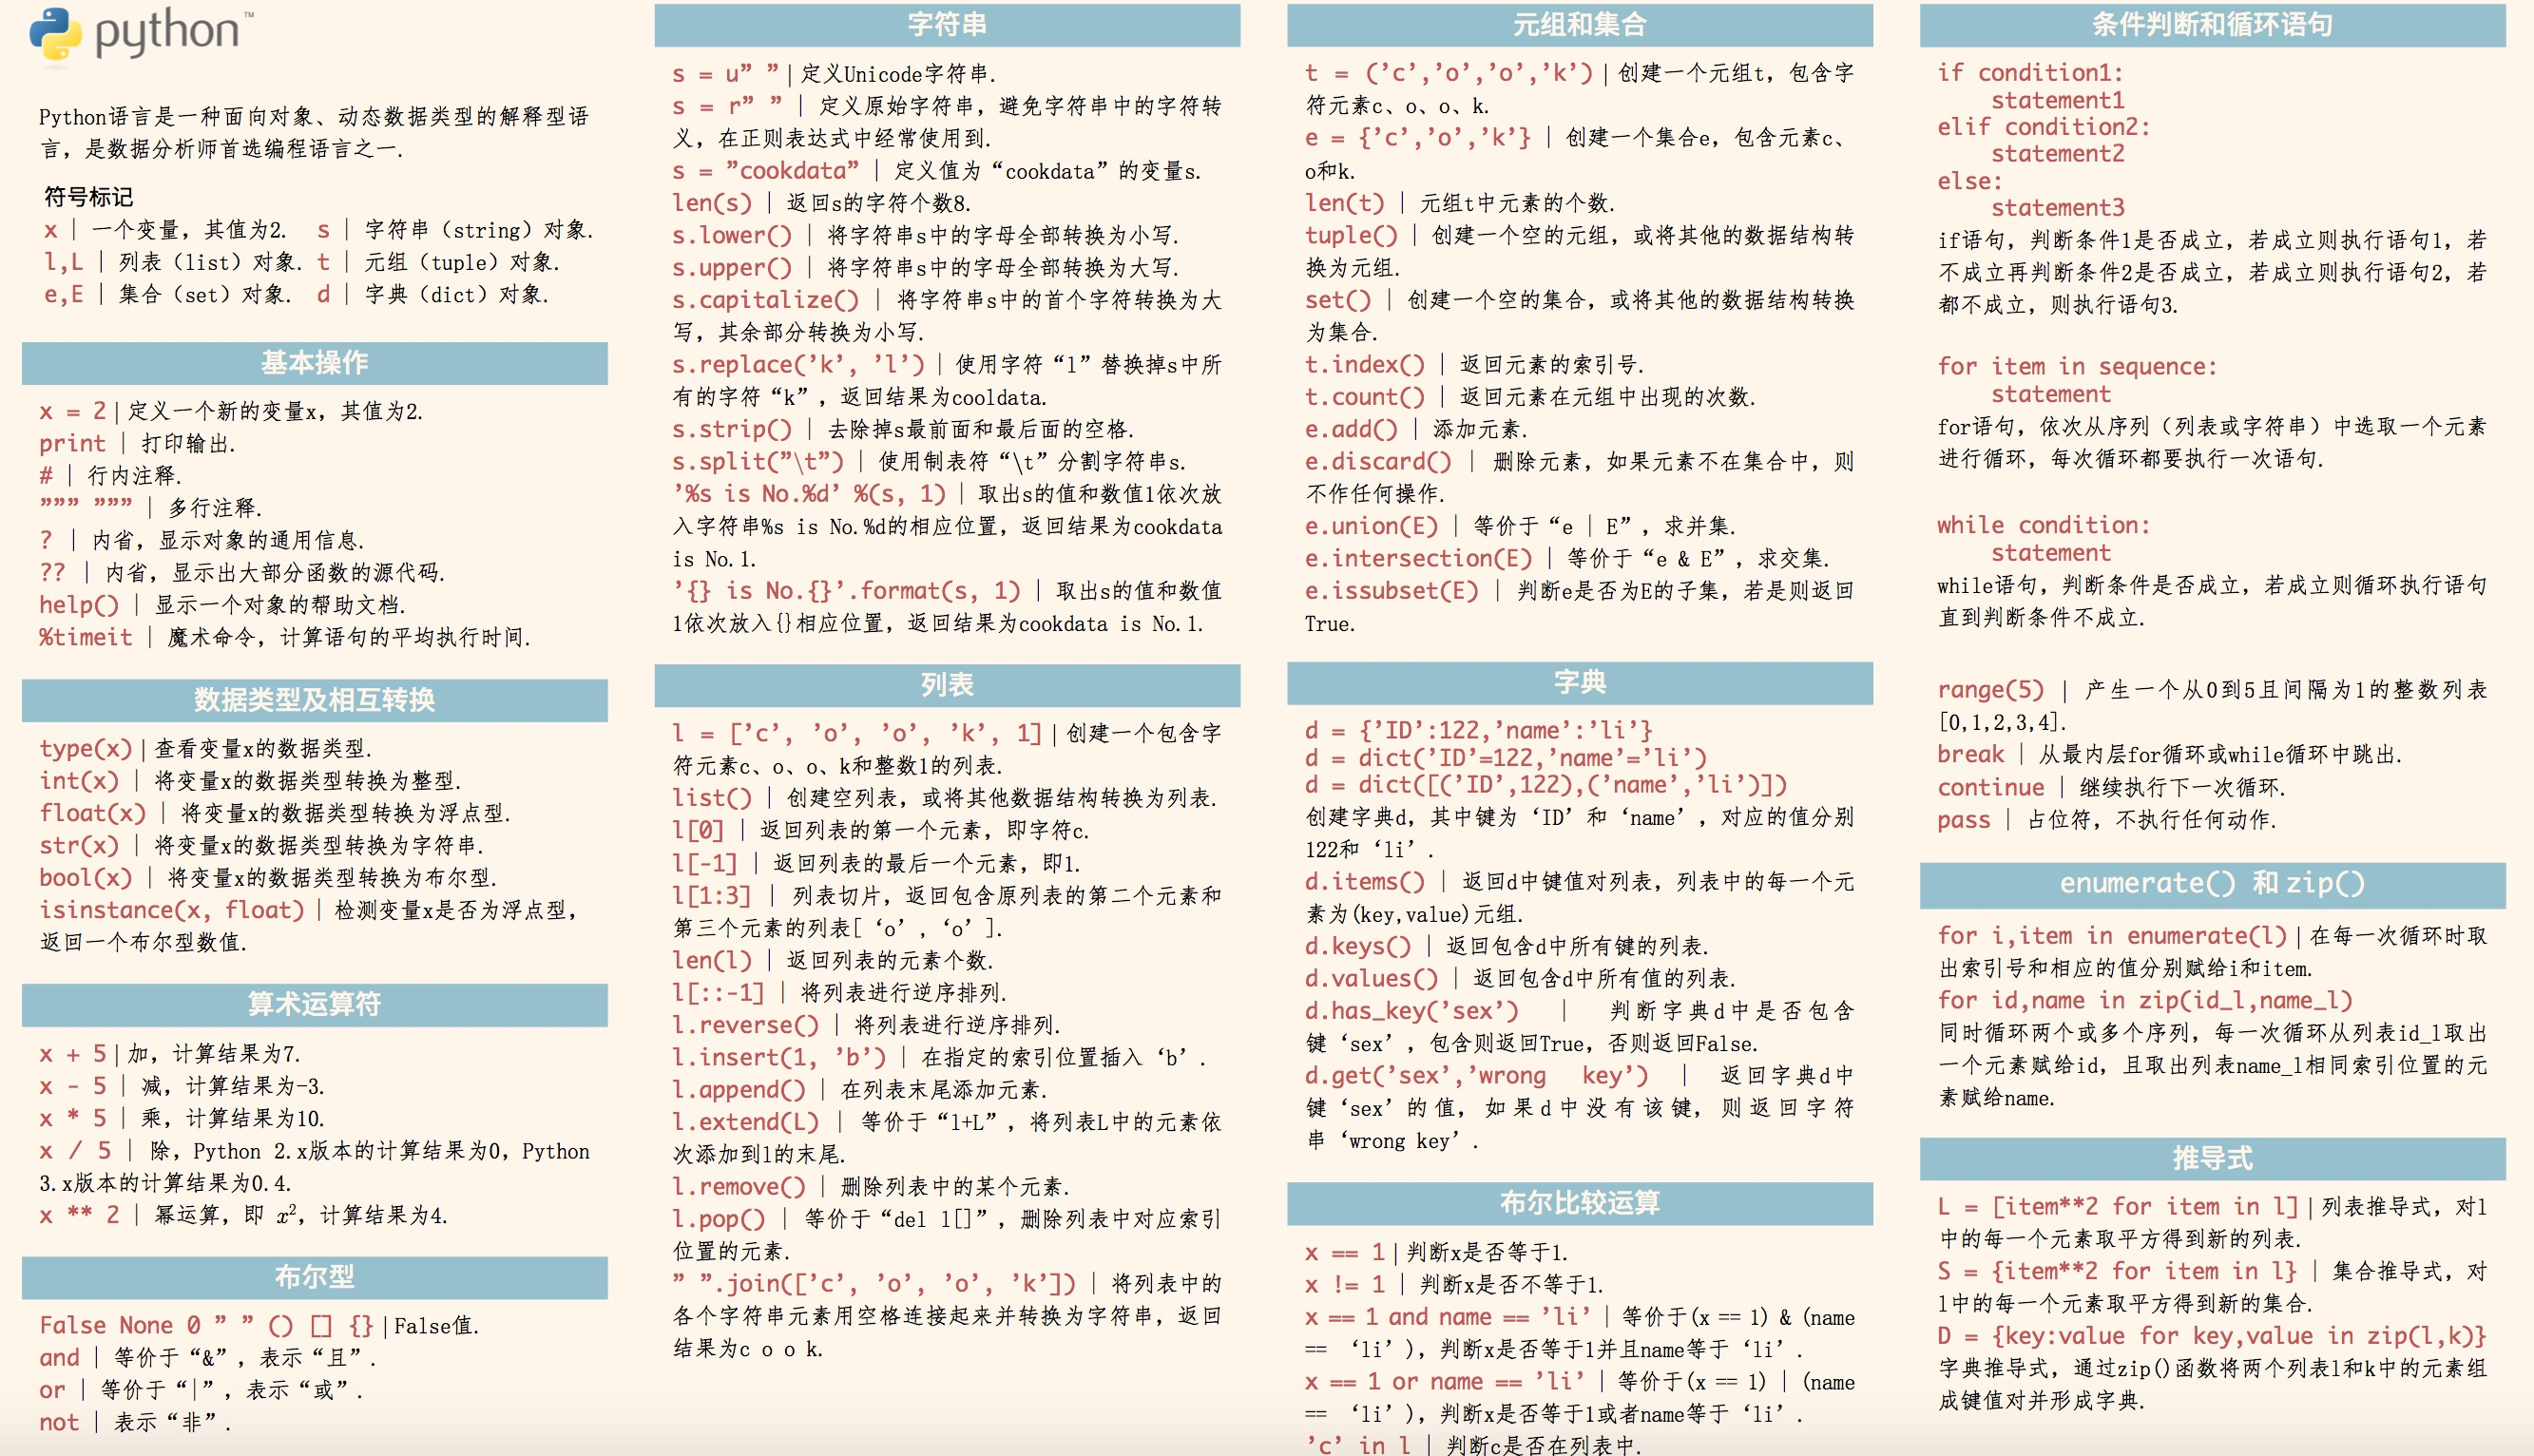
\includegraphics{./python-cheatsheet1.png}
高版本中用\texttt{\textquotesingle{}sex\textquotesingle{}\ in\ d}而不用\texttt{d.has\_key(\textquotesingle{}sex\textquotesingle{})}
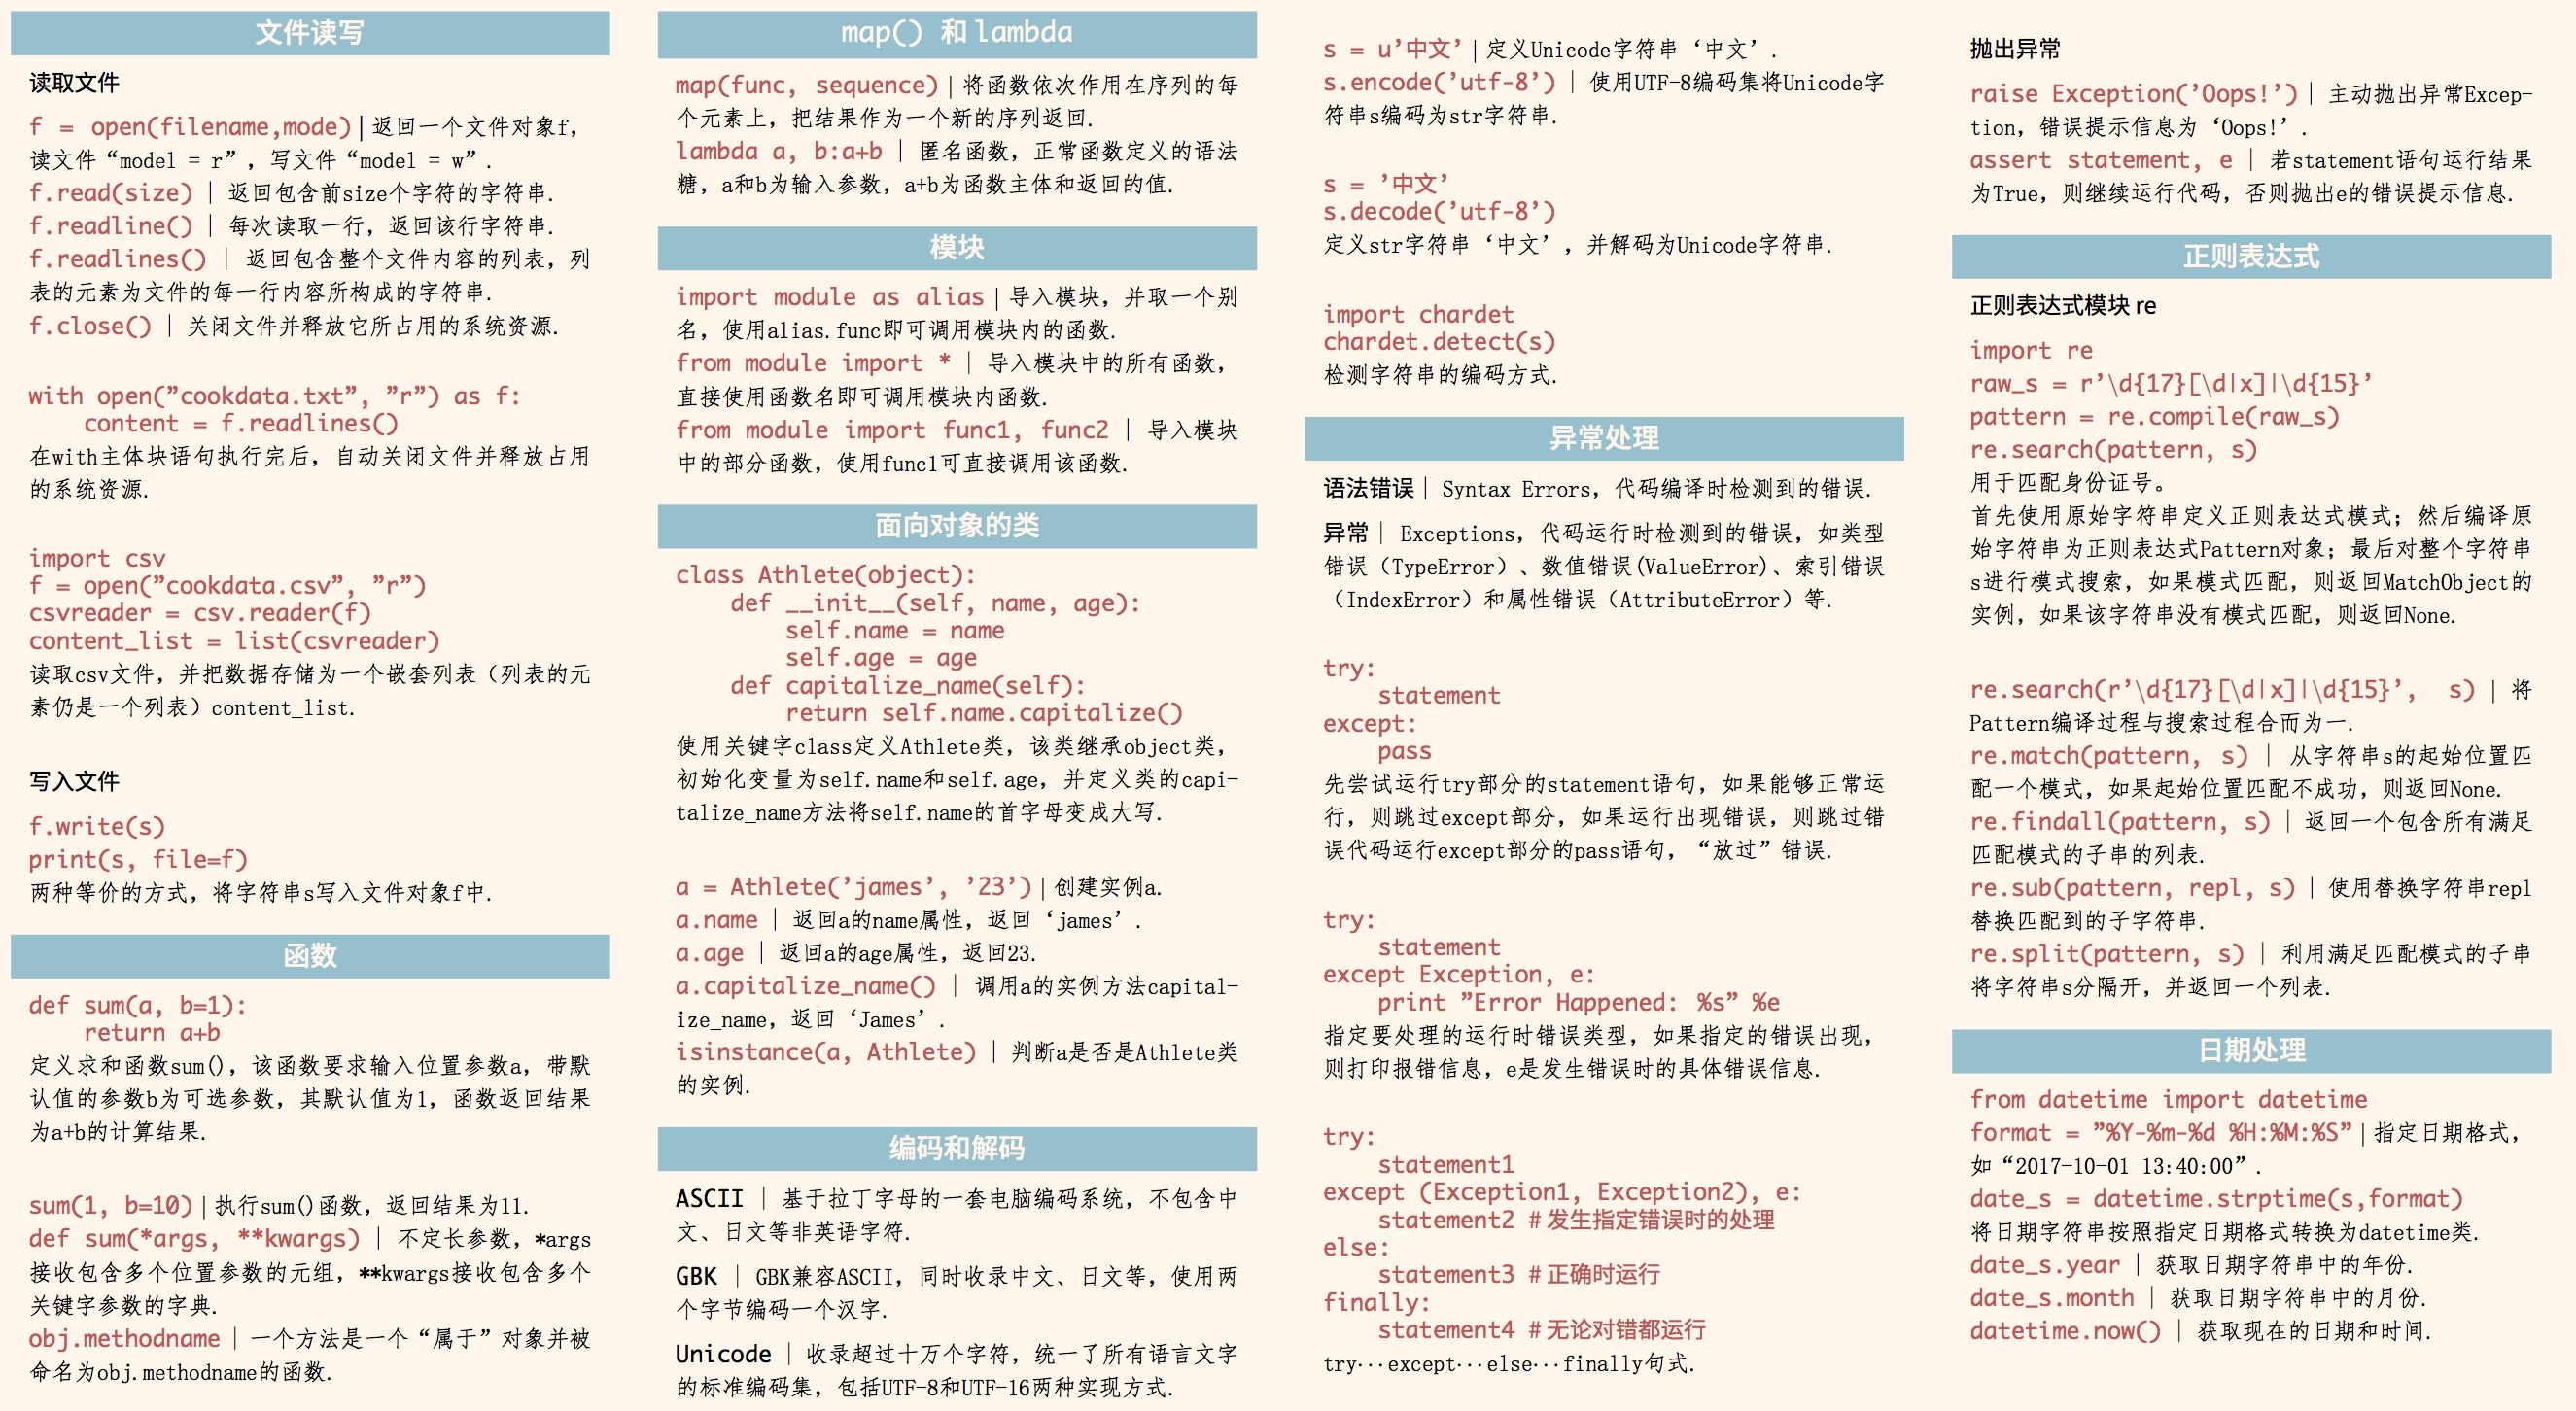
\includegraphics{./python-cheatsheet2.png} python3中try用以下写法

\begin{verbatim}
try:
    statement
except Exception as e:
    print("Error happen...")
\end{verbatim}


    % Add a bibliography block to the postdoc
    
    
    
    \end{document}
